\documentclass{article}
\usepackage[margin=2cm]{geometry}
\usepackage{float}
\usepackage{graphicx}
\usepackage{hyperref}
\usepackage{lscape}
\usepackage{pdflscape}


% Paragraph settings
\setlength{\parskip}{10pt plus 1pt minus 1pt
\setlength{\parindent}{0cm}}

\begin{document}
\title{CS22310 - Hotel Site Assignment}
\author{Samuel Jackson \\ \texttt{slj11@aber.ac.uk}}
\date{\today}
\maketitle

\section{Introduction}
This document provides the final report for the CS22310 Hotel Site assignment and contains the task analysis, interaction design, documentation of prototype and discussion of usability principles. The prototype implementation for this site can be found at \url{http://users.aber.ac.uk/slj11/cs22310/index.html}

\section{Task Analysis}
This section of the document details the analysis of the brief and the identification for the major tasks that the system needs to perform along with characterisation of the users that will perform these tasks. The analysis is documented using a rich picture, use case, data flow and state transition diagrams along with an accompanying description of each.

\subsection{Rich Picture and Identification of Users}
For the first step in my task analysis, I created a rich picture to provide a high level overview of the proposed system and try and identify its major functions and users.

\begin{figure}[H]
\centering
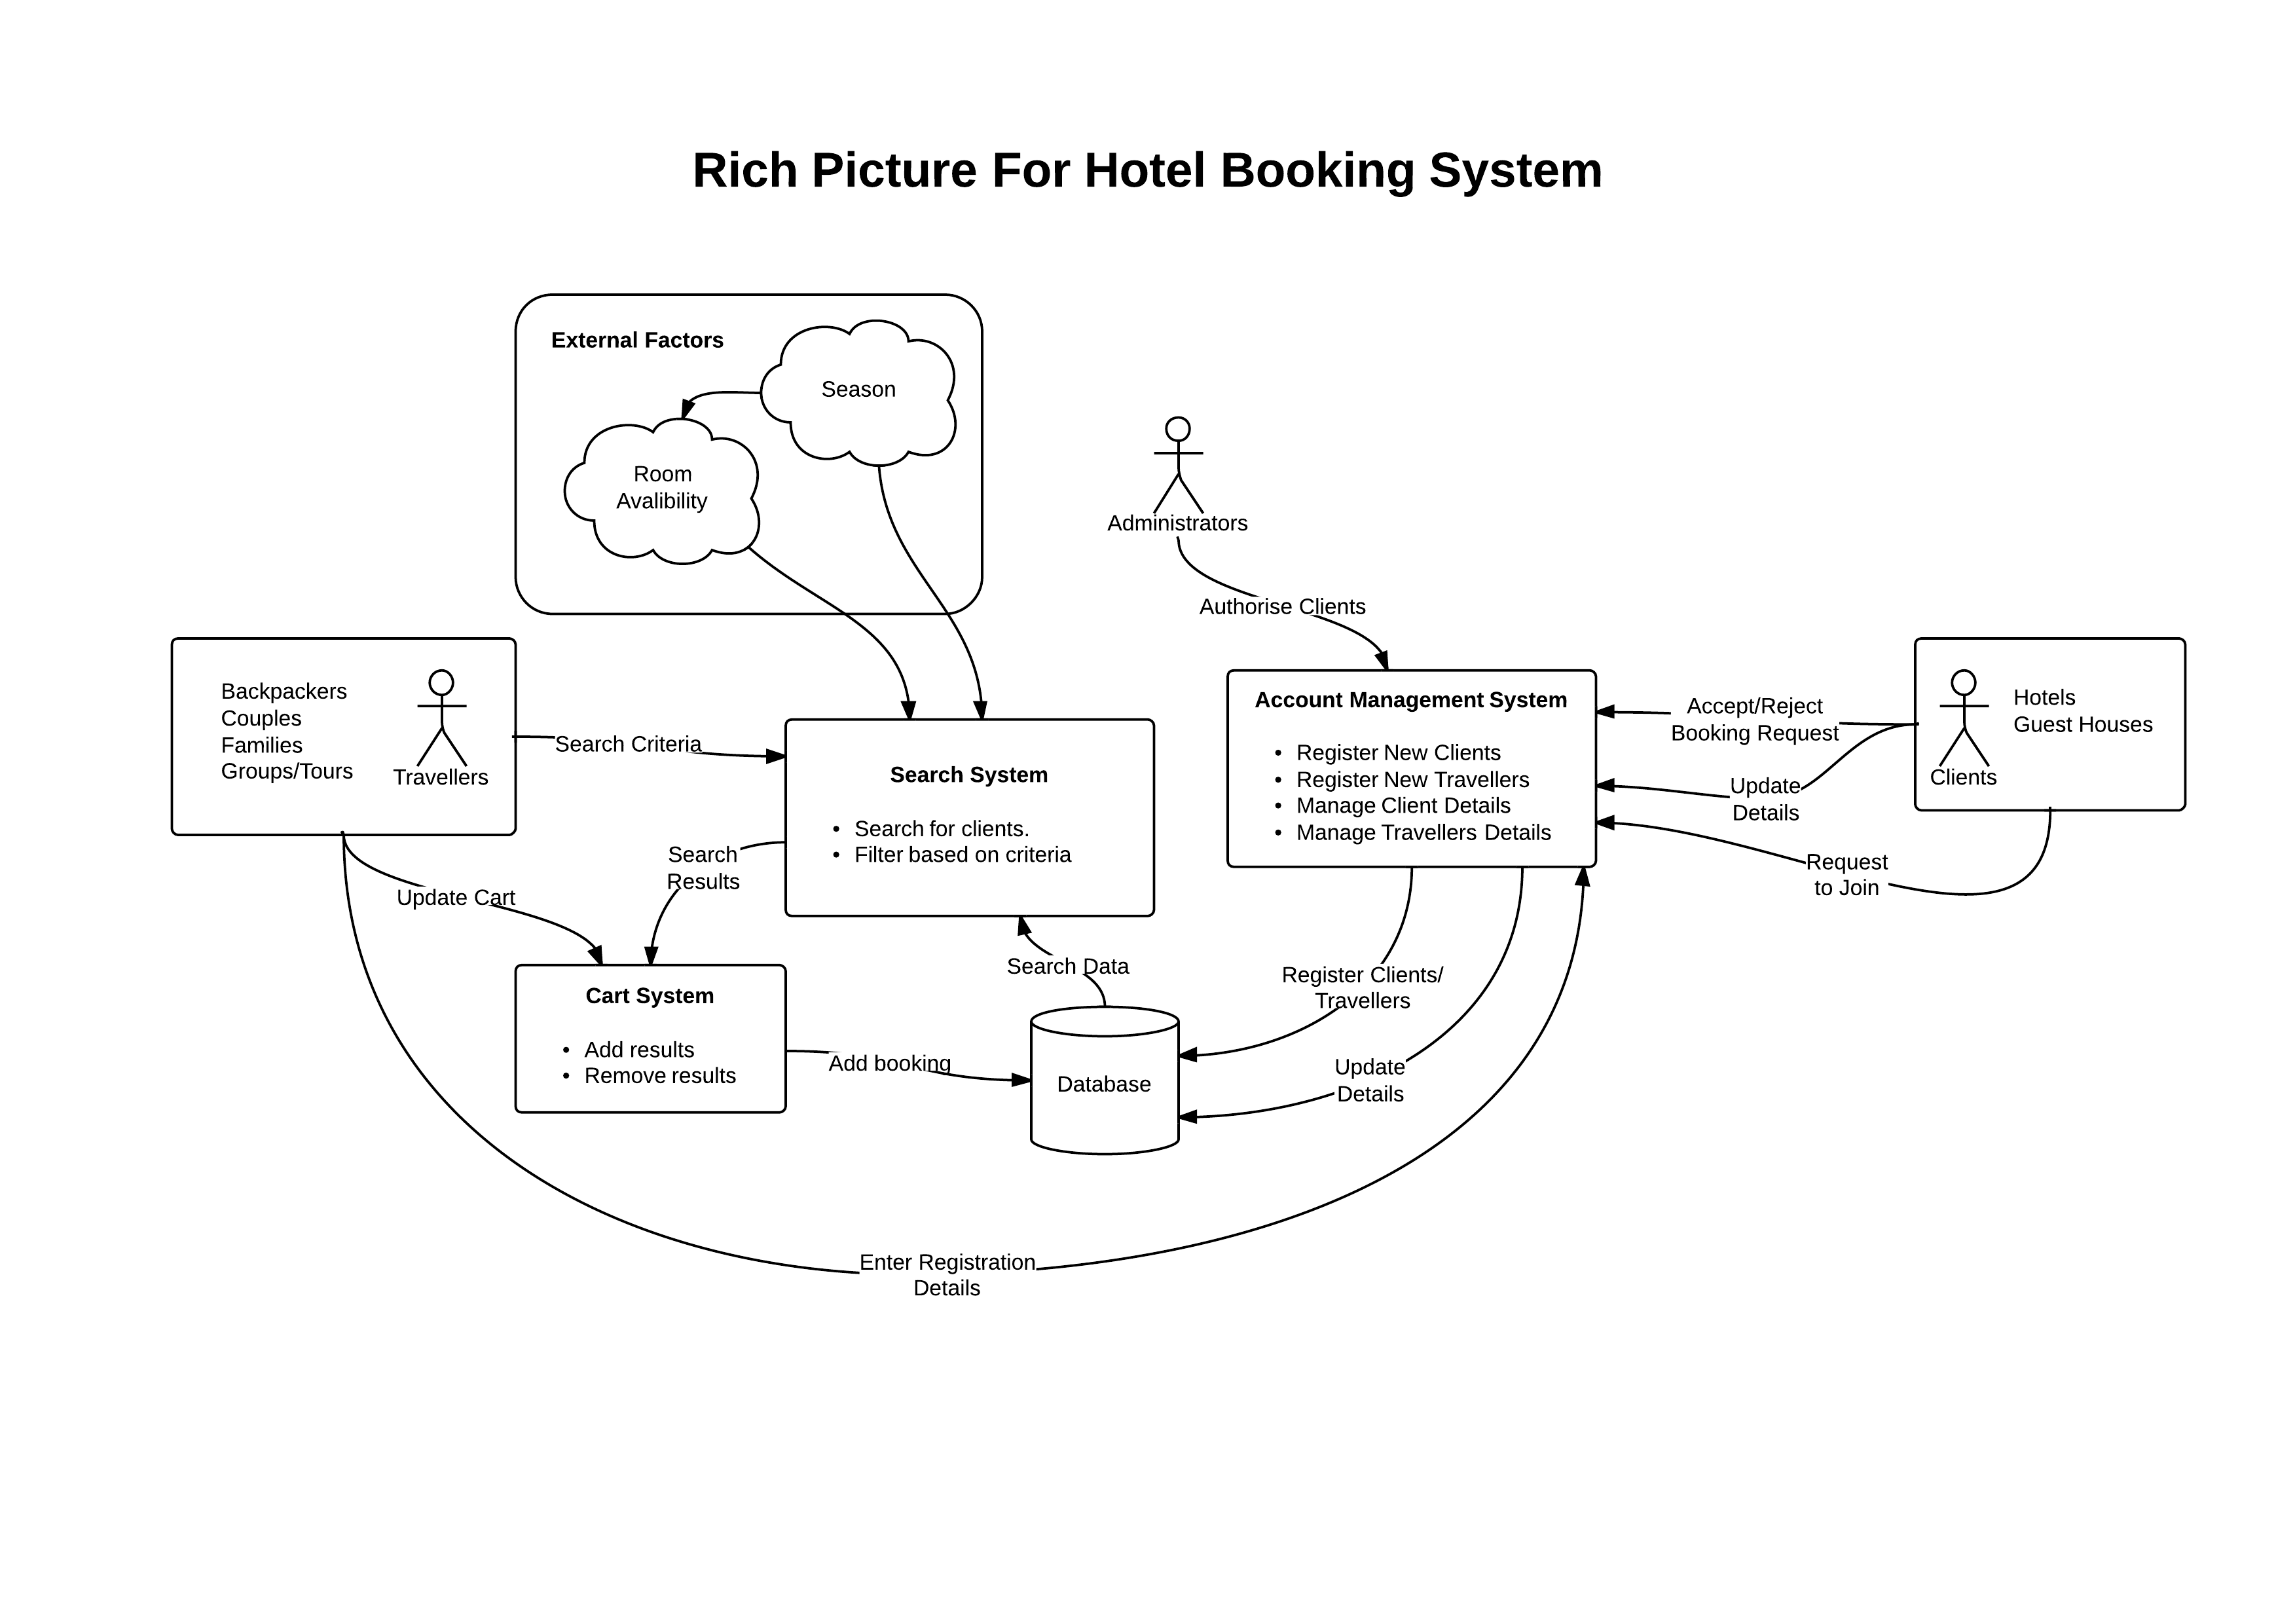
\includegraphics[width=1\textwidth]{img/richpic.png}
\caption{Rich Picture for the Hotel Site}
\label{fig:rich-pic}
\end{figure}

In this diagram, I have identified three key users of the system and three major "task areas" that our system must be able to perform. The major actors in the system are as follows:
\begin{itemize}
	\item \textbf{Travellers} - Travellers are customers of the hotel booking site who wish to search and book lodging with the hotels and guest houses listed on the site.
	\item \textbf{Clients} - Clients are also customers of the hotel booking site, but are representatives or managers of various hotels and guest houses which can register an account with the site to list there available accommodation.
	\item \textbf{Administrators} - Administrators are employees of the hotel booking site and who's only major function is to authorise requests by clients for registration with the site.
\end{itemize}

Of the three major types of users identified here, the most technologically inexperienced are most likely to be the Travellers. This is due to the potentially wide variety of different customers that could use the site as this a diverse user demographic implies a wide diversity in technological competency. They  will also have almost no training in how to use the system (unlike administrators and possibly clients). It is therefore paramount that system functions undertaken by Travellers be as clear and accessible as possible. Travellers may be either single contact (they only use the site once) or may be repeat customers. Therefore there interface should accommodate inexperienced "first time" users while still providing ease of access for power users.

Clients are likely to be similar to travellers, but perhaps with slightly less diversity in competency. This is due to the fact that the hotel/guest house may have a dedicated member of staff (such as a manager) that is responsible for dealing with the management of hotel's listing on the site. This employee may also receive training by an employee which already knows how to use the system. However, when a new client registers with the hotel site, the client management interface stills needs to be intuitive to the first time users. This point is particularly relevant the smaller hotels and guest houses who are more likely to not have a technical professional to handle the establishments web presence.

Client will have a recurring connection with hotel site and there connection is most likely going to last for months and years, rather than being a single one off connection with the site like some potential Travellers. Again it is stressed that this section of the site be accessible to a variety of user skill levels. It is also more of a requirement that this part of the site be efficient. Client users are not looking to "browse" like Travellers but are coming to the site to perform a specific task (e.g. updating promotional information) and therefore want clear and easy to use interface to quick accomplish the task the came to do.

The final major type of system user are administrators. Administrators are likely to be the most technically competent users. They are expected to have frequent, recurrent contact with the system, probably on a daily basis. They are also likely to be well trained by the company running the hotel booking site. Like Clients, they will not wish to "browse" the site, but will come to it in order to carry out a specific task and therefore will want a clear and efficient interface suitable for a power user.

The rich picture also identifies three key categories that user tasks fall into across the site. The first category of task are those related to the management of the accounts associated with users. This includes tasks that allow the Clients to update information about their establishment, the registration of Client and Travellers and Travellers updating their payment and billing information. Task in this category are carried out by each of the types of system users.

In contrast, the other two categories that system tasks fall into are only carried out by Travellers. These two areas are the search system and the cart/payment system. Both of these areas are distinct but closely related. In fact, the search system feeds into the cart and payment system. However, the search system is concerned with getting results that match the users criteria and refining there choices. The cart system is designed to guide the user through the payment and booking process after they have finished making their choices. Note that the picture also displays some external influences on the search system which ma affect the results available to Travellers, such as room availability and the season.

As a final note, I have also added the a data store labelled database. This is the major data sink on the hotel site server where information about bookings, hotel and user accounts all feed into. Data is pulled from this store and displayed via the interface as required.

\subsection{System Tasks}
The next step in task analysis is to analyse, at a high level, the actions that can be performed by each of the identified users within the system. In order to clear identify each of these actions, the following use case diagram is provided.

\begin{figure}[H]
\centering
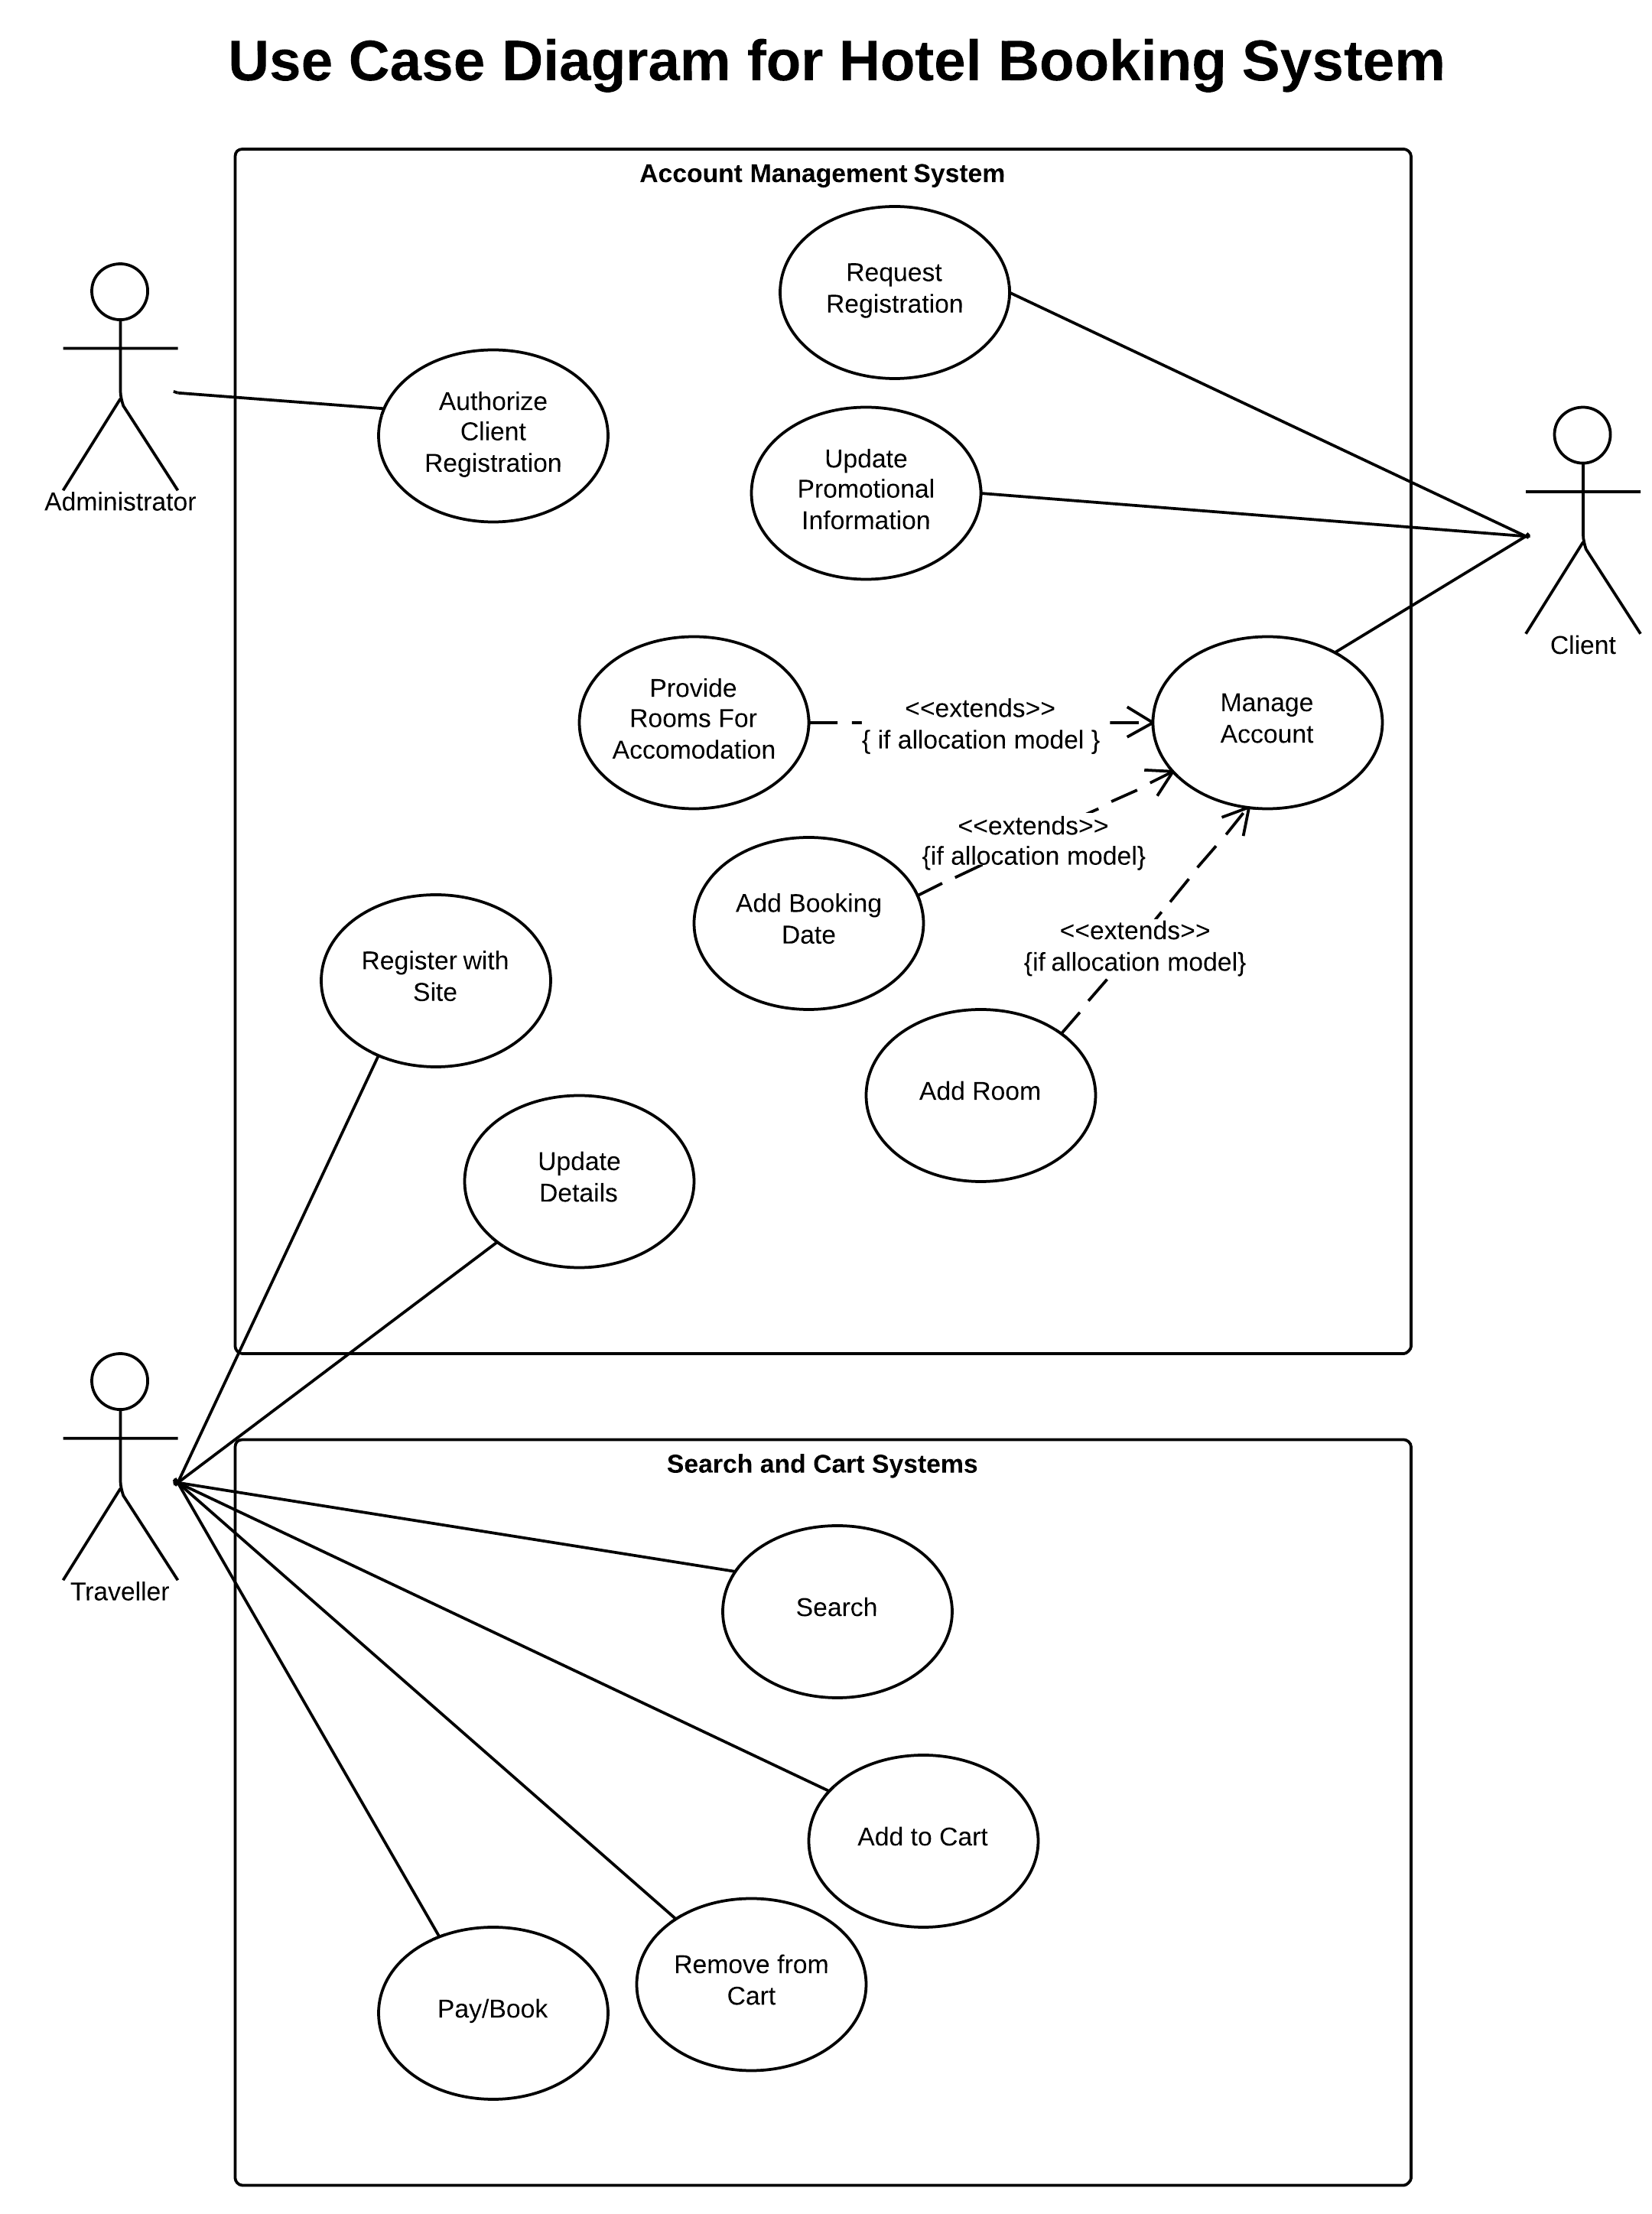
\includegraphics[width=1\textwidth]{img/UseCase.png}
\caption{Use Case diagram for the Hotel Site. Inc. all major actors.}
\label{fig:use-case}
\end{figure}

In figure \ref{fig:use-case}, the tasks each user can perform have been split into two sections. One outlining tasks to do with the management of a users account, and one to do with the actions of find and booking a hotel.

The major tasks a client can perform within the system are to request registration, update promotional information and manage their account. A client cannot directly register with the system. They must first make a request for registration which will later we authorised or declined by a system administrator. It is during this action that the client would be expected to provide details of which type of membership they require (e.g. allocation or referral model).

Updating promotional information fairly self explanatory. Clients will have the ability to change the description about their site that is displayed to travellers on the front end of the site.

Management of a client's account is a fairly broad task that encapsulates how clients can update the information about their site depending of the type of account they are given. If they are registered with a referral account, booking request details will be send to them via an automated email from the site. It is then the clients responsibility to respond to these requests. However, if the Client has a allocation type account, they will be able to update the number of rooms they have listed on the site, along with the dates which each of the rooms is booked for.

Travellers can perform tasks in both areas of the site. They have the ability to register with the site (no authorisation required) and can update their personal details stored with the site such as their card number and billing address.

They can also perform a variety of actions in relation to the search and cart systems such as search for a hotel based on a given criteria, adding/removing items to there cart and paying for the items in the cart when ready.

\subsection{Data Flow Diagram}
The next step in task analysis was to plan how data could possible flow between  actors, system tasks and data stores. I have provided the following data flow diagram to show how data might flow between the users and the tasks being performed by the booking site.

\begin{landscape}
\begin{figure}[H]
\centering
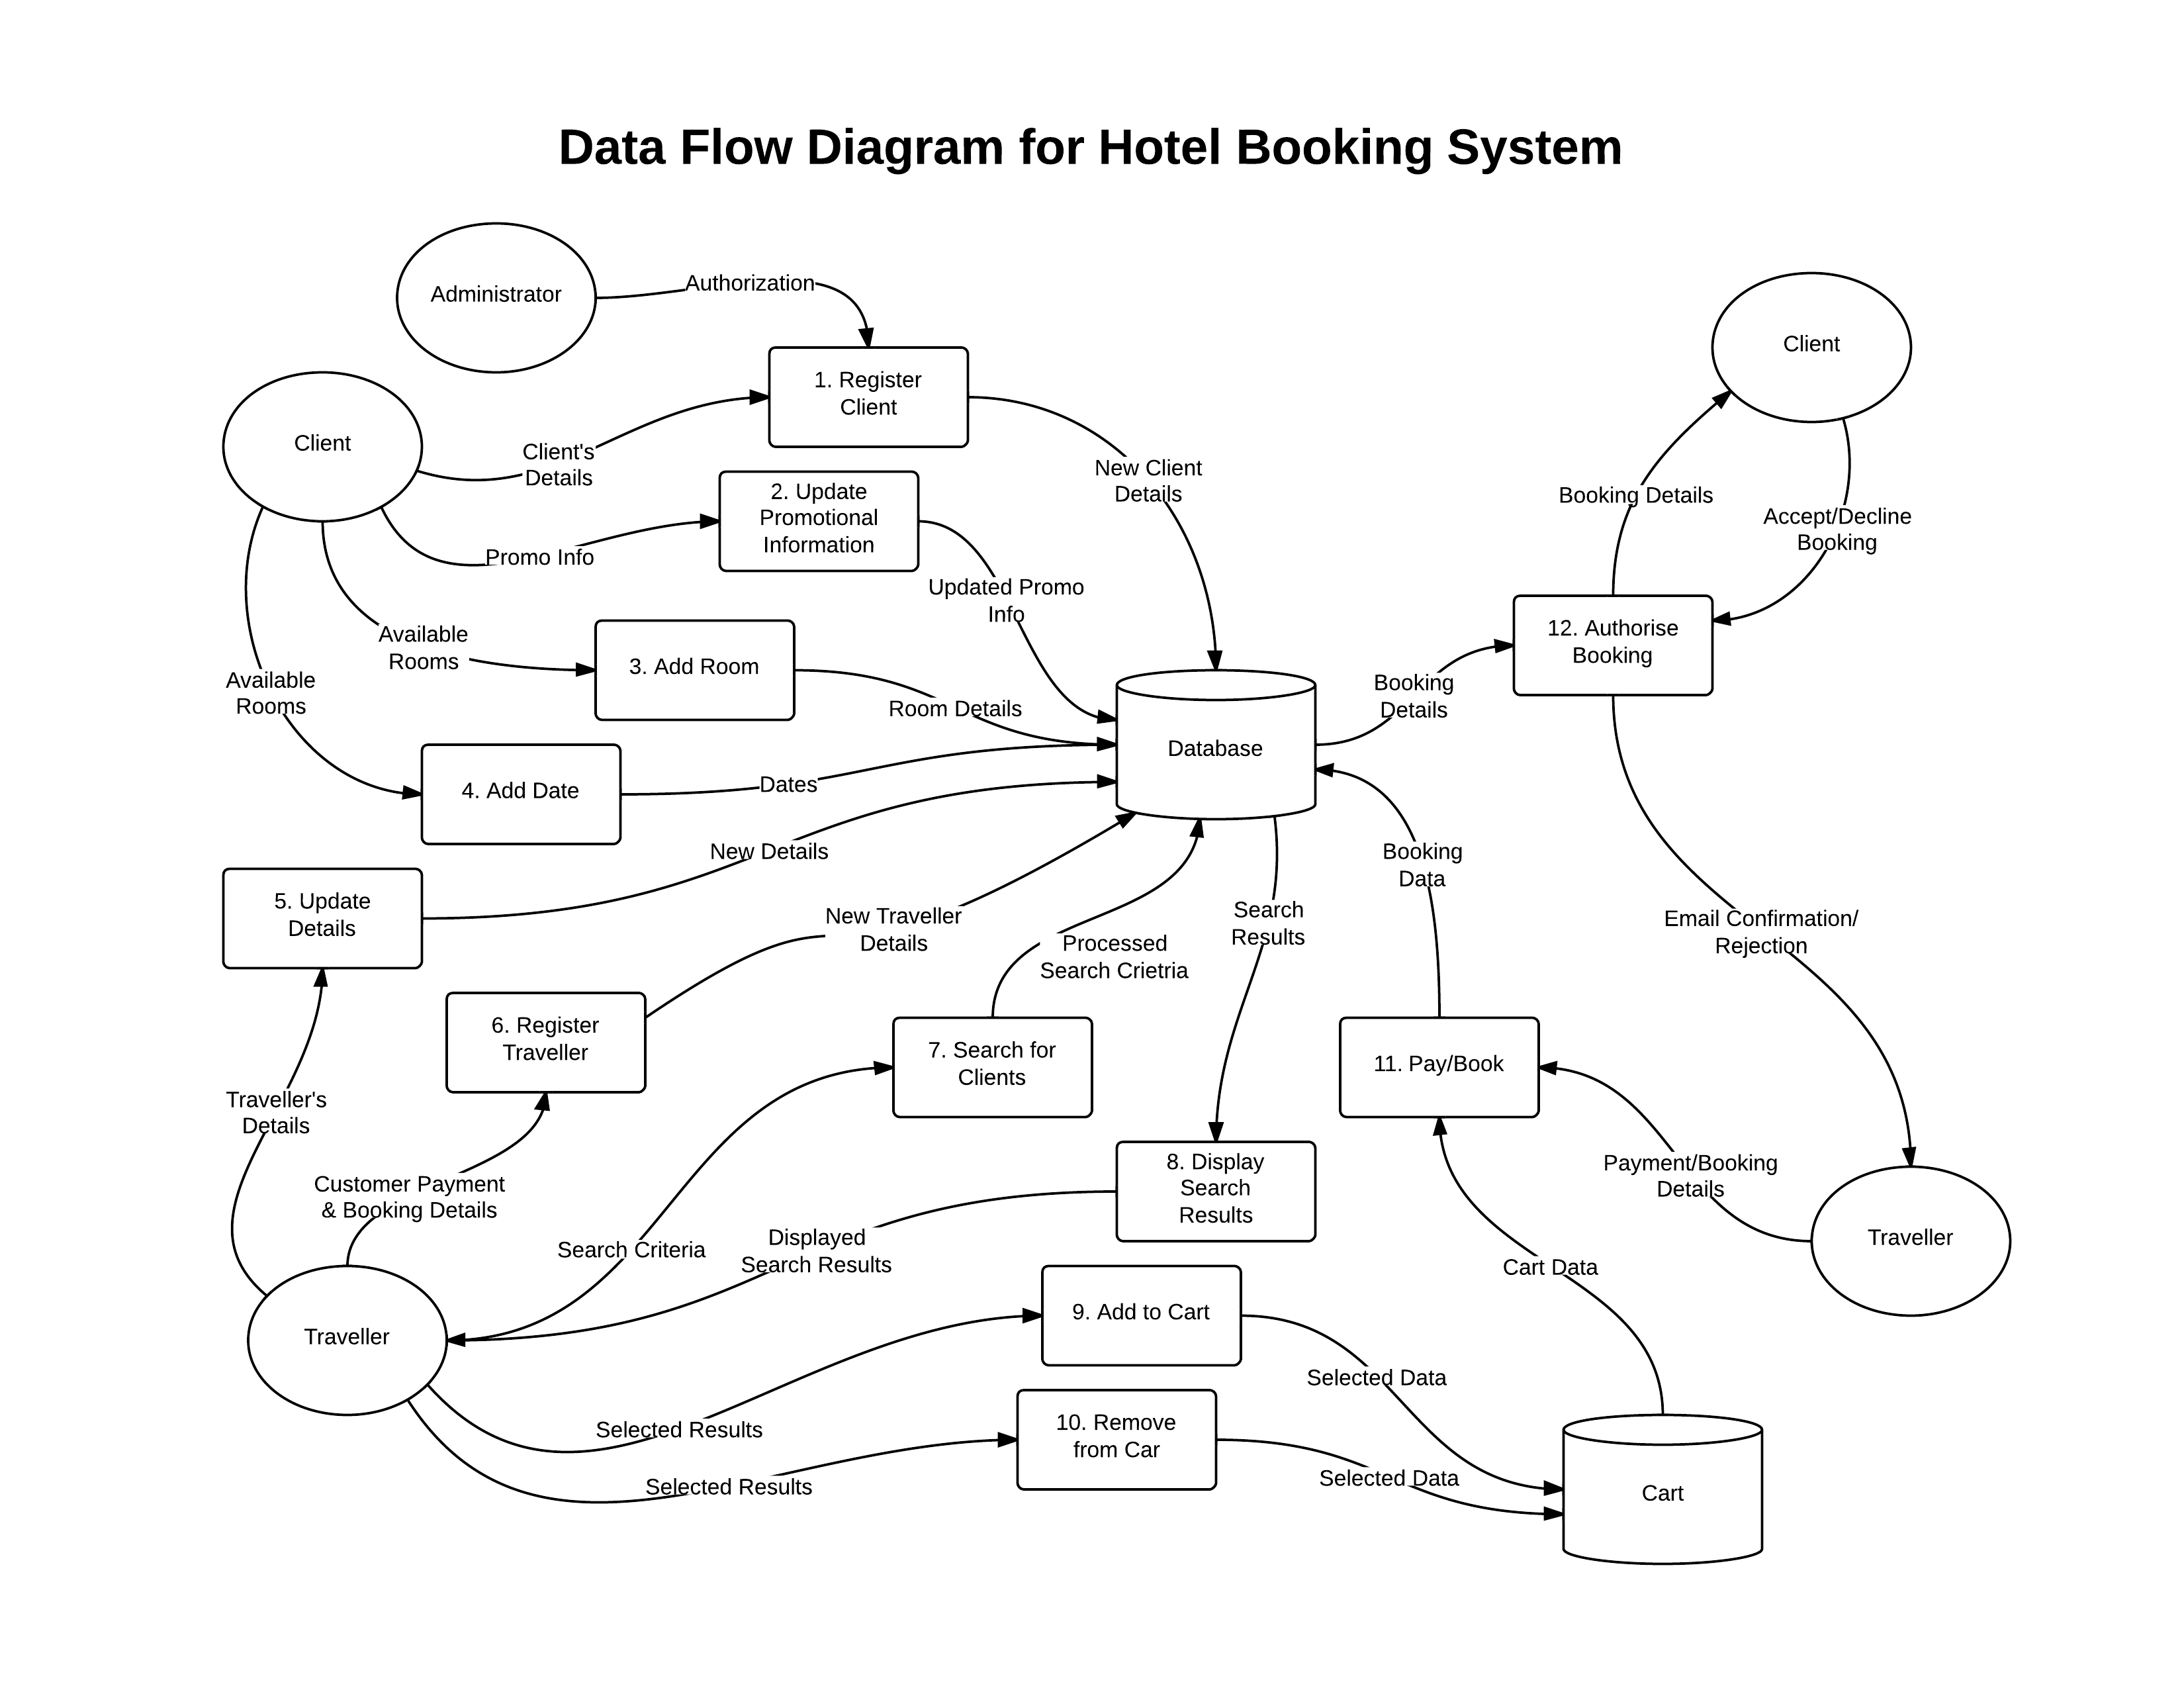
\includegraphics[angle=0, width=1\textwidth]{img/dataflow.png}
\caption{Data flow diagram for the Hotel Booking site.}
\label{fig:data-flow}
\end{figure}
\end{landscape}

Each of the major tasks identified in the use case analysis is shown, along with a bit more detail. Note that this diagram shows the flow of data for both the allocation and referral models as there are only a couple of differences between the two models. If a client is using the allocation model, The authorise booking stage would not be present as the booking would be completed automatically by the Hotel Site system and would therefore be unnecessary. Likewise, the ability for a client to add a room and add a booking date would not be present if the Client is assigned to the referral model.

Note that in this diagram I have visualised the cart as being a separate data store from the database. In an actual implementation, they would mostly likely be part of the same relational database model. However, I have decided to logically separate them here for clarity.

\subsection{State Transition Diagrams}
The final step in task analysis was to identify on a low level how the user can move between states in the system. For this section I provide a collection of state transition diagrams. These help to illustrate how users can move through a system to carry out desired tasks. The states shown also help to point out good possible starting points for the page designs outlined in the next section.

\begin{figure}[H]
\centering
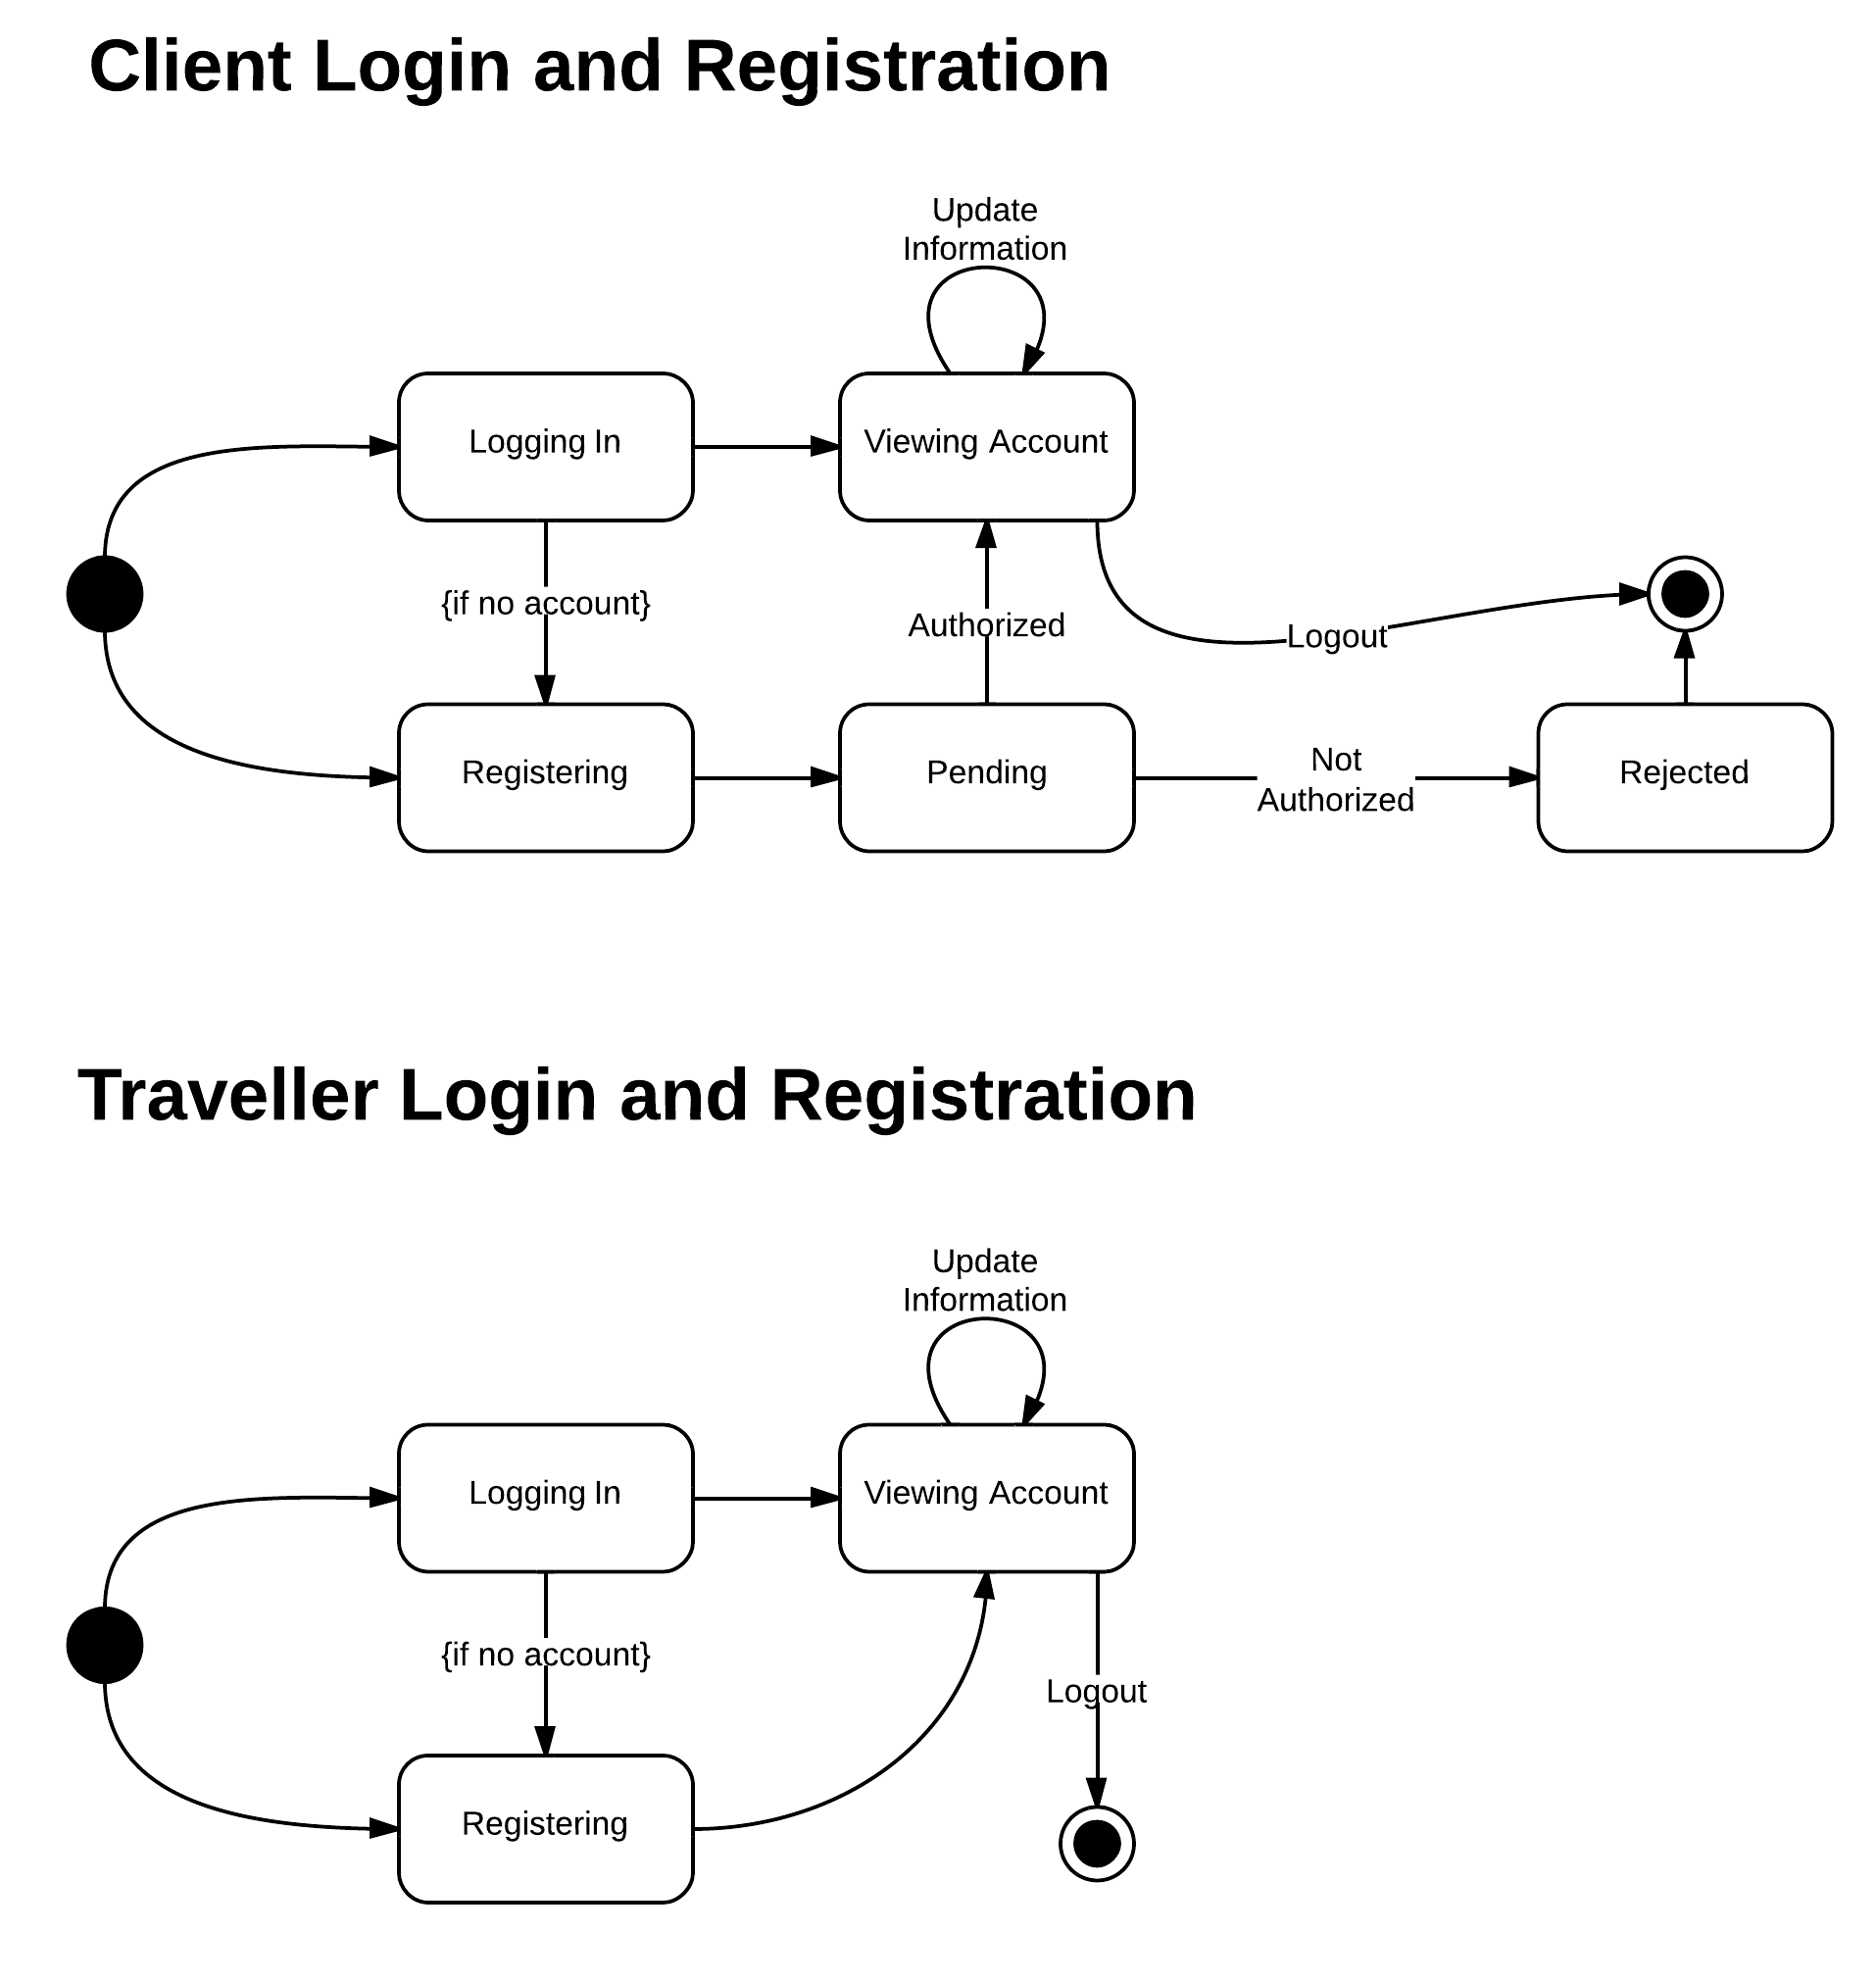
\includegraphics[width=0.7\textwidth]{img/state_diagrams/StateDiagramUserAuth.png}
\caption{State Transition diagrams for both Client and Traveller Login and Registration}
\label{fig:state-user-auth}
\end{figure}

Figure \ref{fig:state-user-auth} shows a comparison between the way that Clients and Travellers sign up for an account with the site and login for the site. In my design, it is planned that if a Client or Traveller attempts to perform an action that requires them to be logged in (such as viewing their account overview) and they have not yet logged in, they will be redirected automatically to the appropriate login page. Also note that Travellers will be required to register for an account or login before they can purchase the items stored in their cart.

Traveller login and registration is a fairly straight forward process. If a Traveller can login they go directly to the view account page. If they do not have an account yet, they can move to the registration page where they can get an account. They will then be diverted to the login page where they can perform further tasks. In the actual implementation, if the Traveller is asked to login/register during the process of buying the items in the cart, they will the not be sent to the account overview page, but redirected back into the buying process.

The Client login and registration process is very similar, but incorporates an extra step in the registration process. Because Client accounts need to be authorised by an administrator before Clients can use the management features, when a client registers they are moved into the pending state until their request for an account is either accepted or declined. Once it is accepted they can then proceed to use account management features.

\begin{figure}[H]
\centering
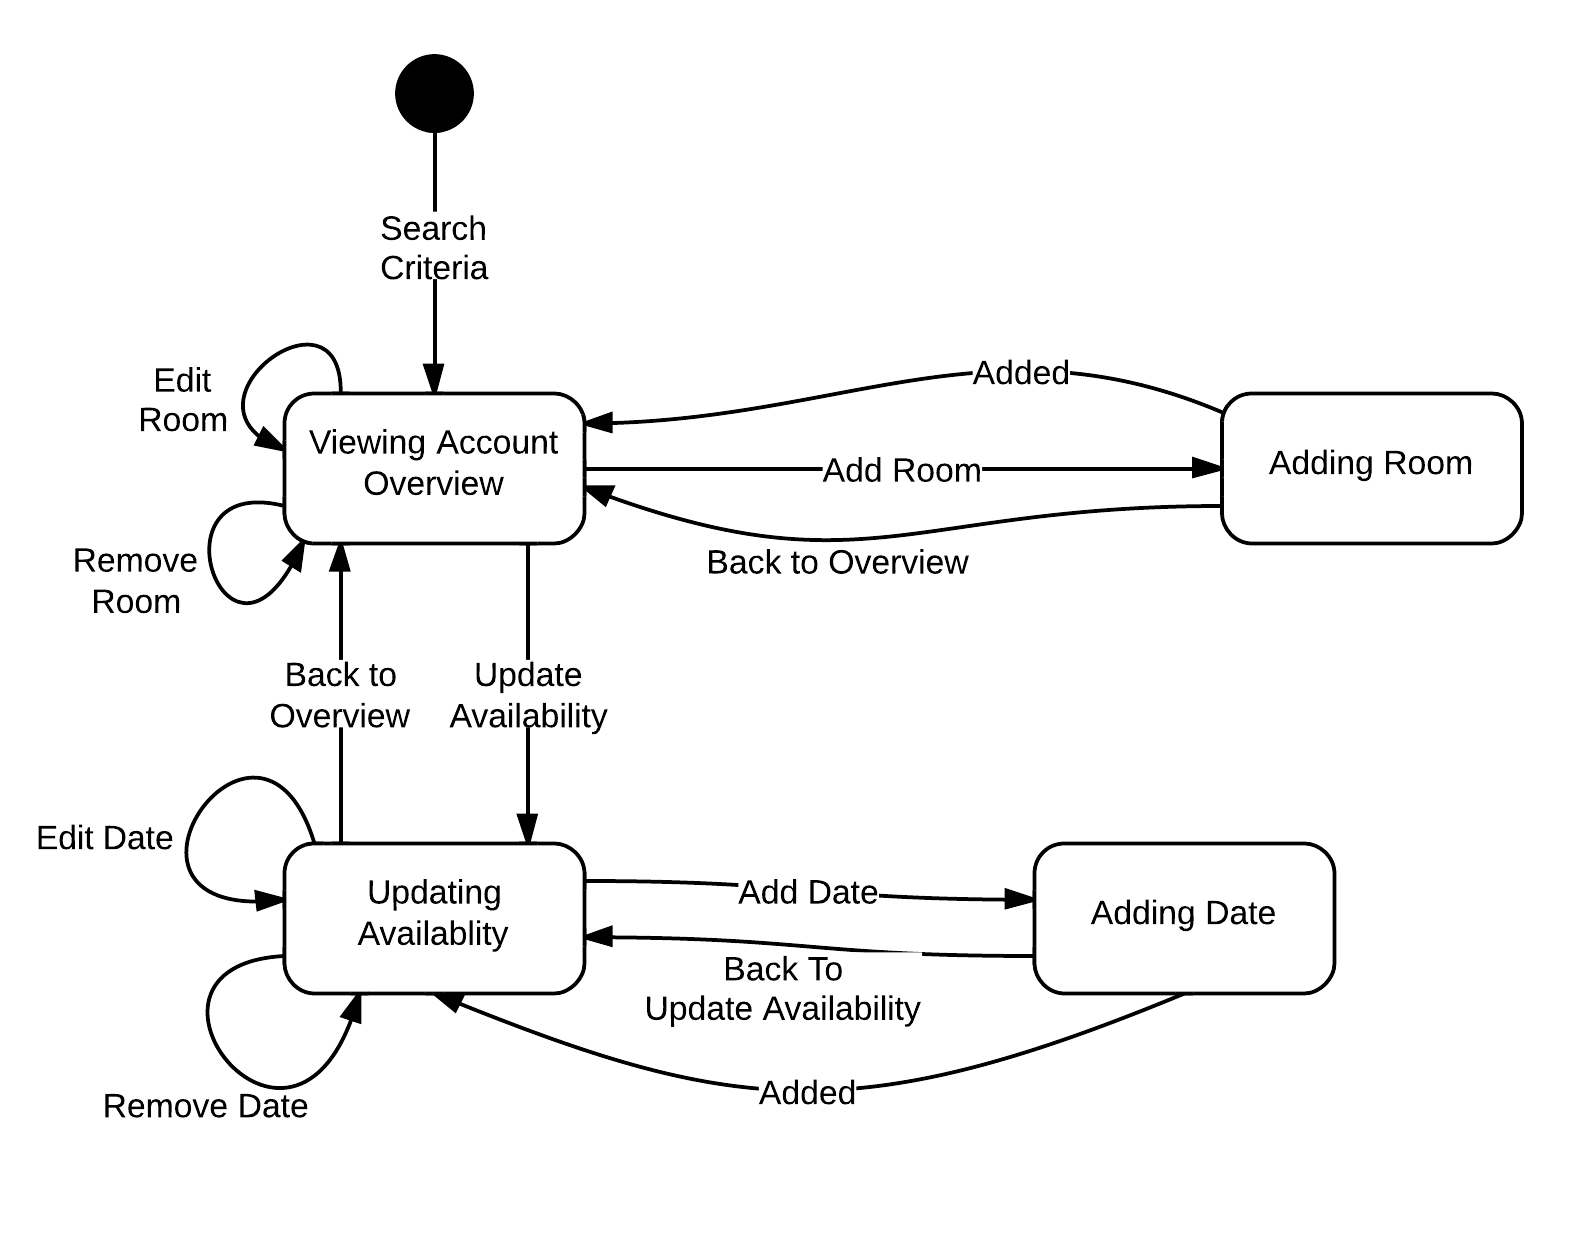
\includegraphics[width=0.7\textwidth]{img/state_diagrams/StateTransitionClientManagement.png}
\caption{State Transition diagram for Client account management}
\label{fig:state-client-manage}
\end{figure}

The next state transition diagram show in figure \ref{fig:state-client-manage} shows how Clients can moved between states of editing details about their account if they are using the allocation model. This state transition diagram is not applicable if the Client is using the referral model. In that case, the only action they are able to perform is the to update their promotional information.

This diagram shows the options a Client has to manage their account in greater detail. Here you can see that they have options to add, edit and remove a room and a booking date associated with a room. Transitions that state back to overview/update availability imply that not change was made to the system in the preceding state.

Each of the states in this diagram ultimately represents a page on the site and correlates to tasks that user might want to perform in this state. Note how editing and removing information does not require a change in state this is because each of the items will displayed in a form, so can be edited directly. In the real system edit and remove operations would mostly likely use AJAX or a simple page refresh to update the users interface after the operation has been carried out.

However, operations that require the user to add new information into the system require a change of state. This is because addition operations will require more information that from the user than an edit or remove operation and I therefore felt that it would be more clear what information was required if the user was moved to another state to breakdown the number of options a Client can choose in any single state. In any single state during Client management, the Client is not presented with more than five possible operations at once.

\begin{figure}[H]
\centering
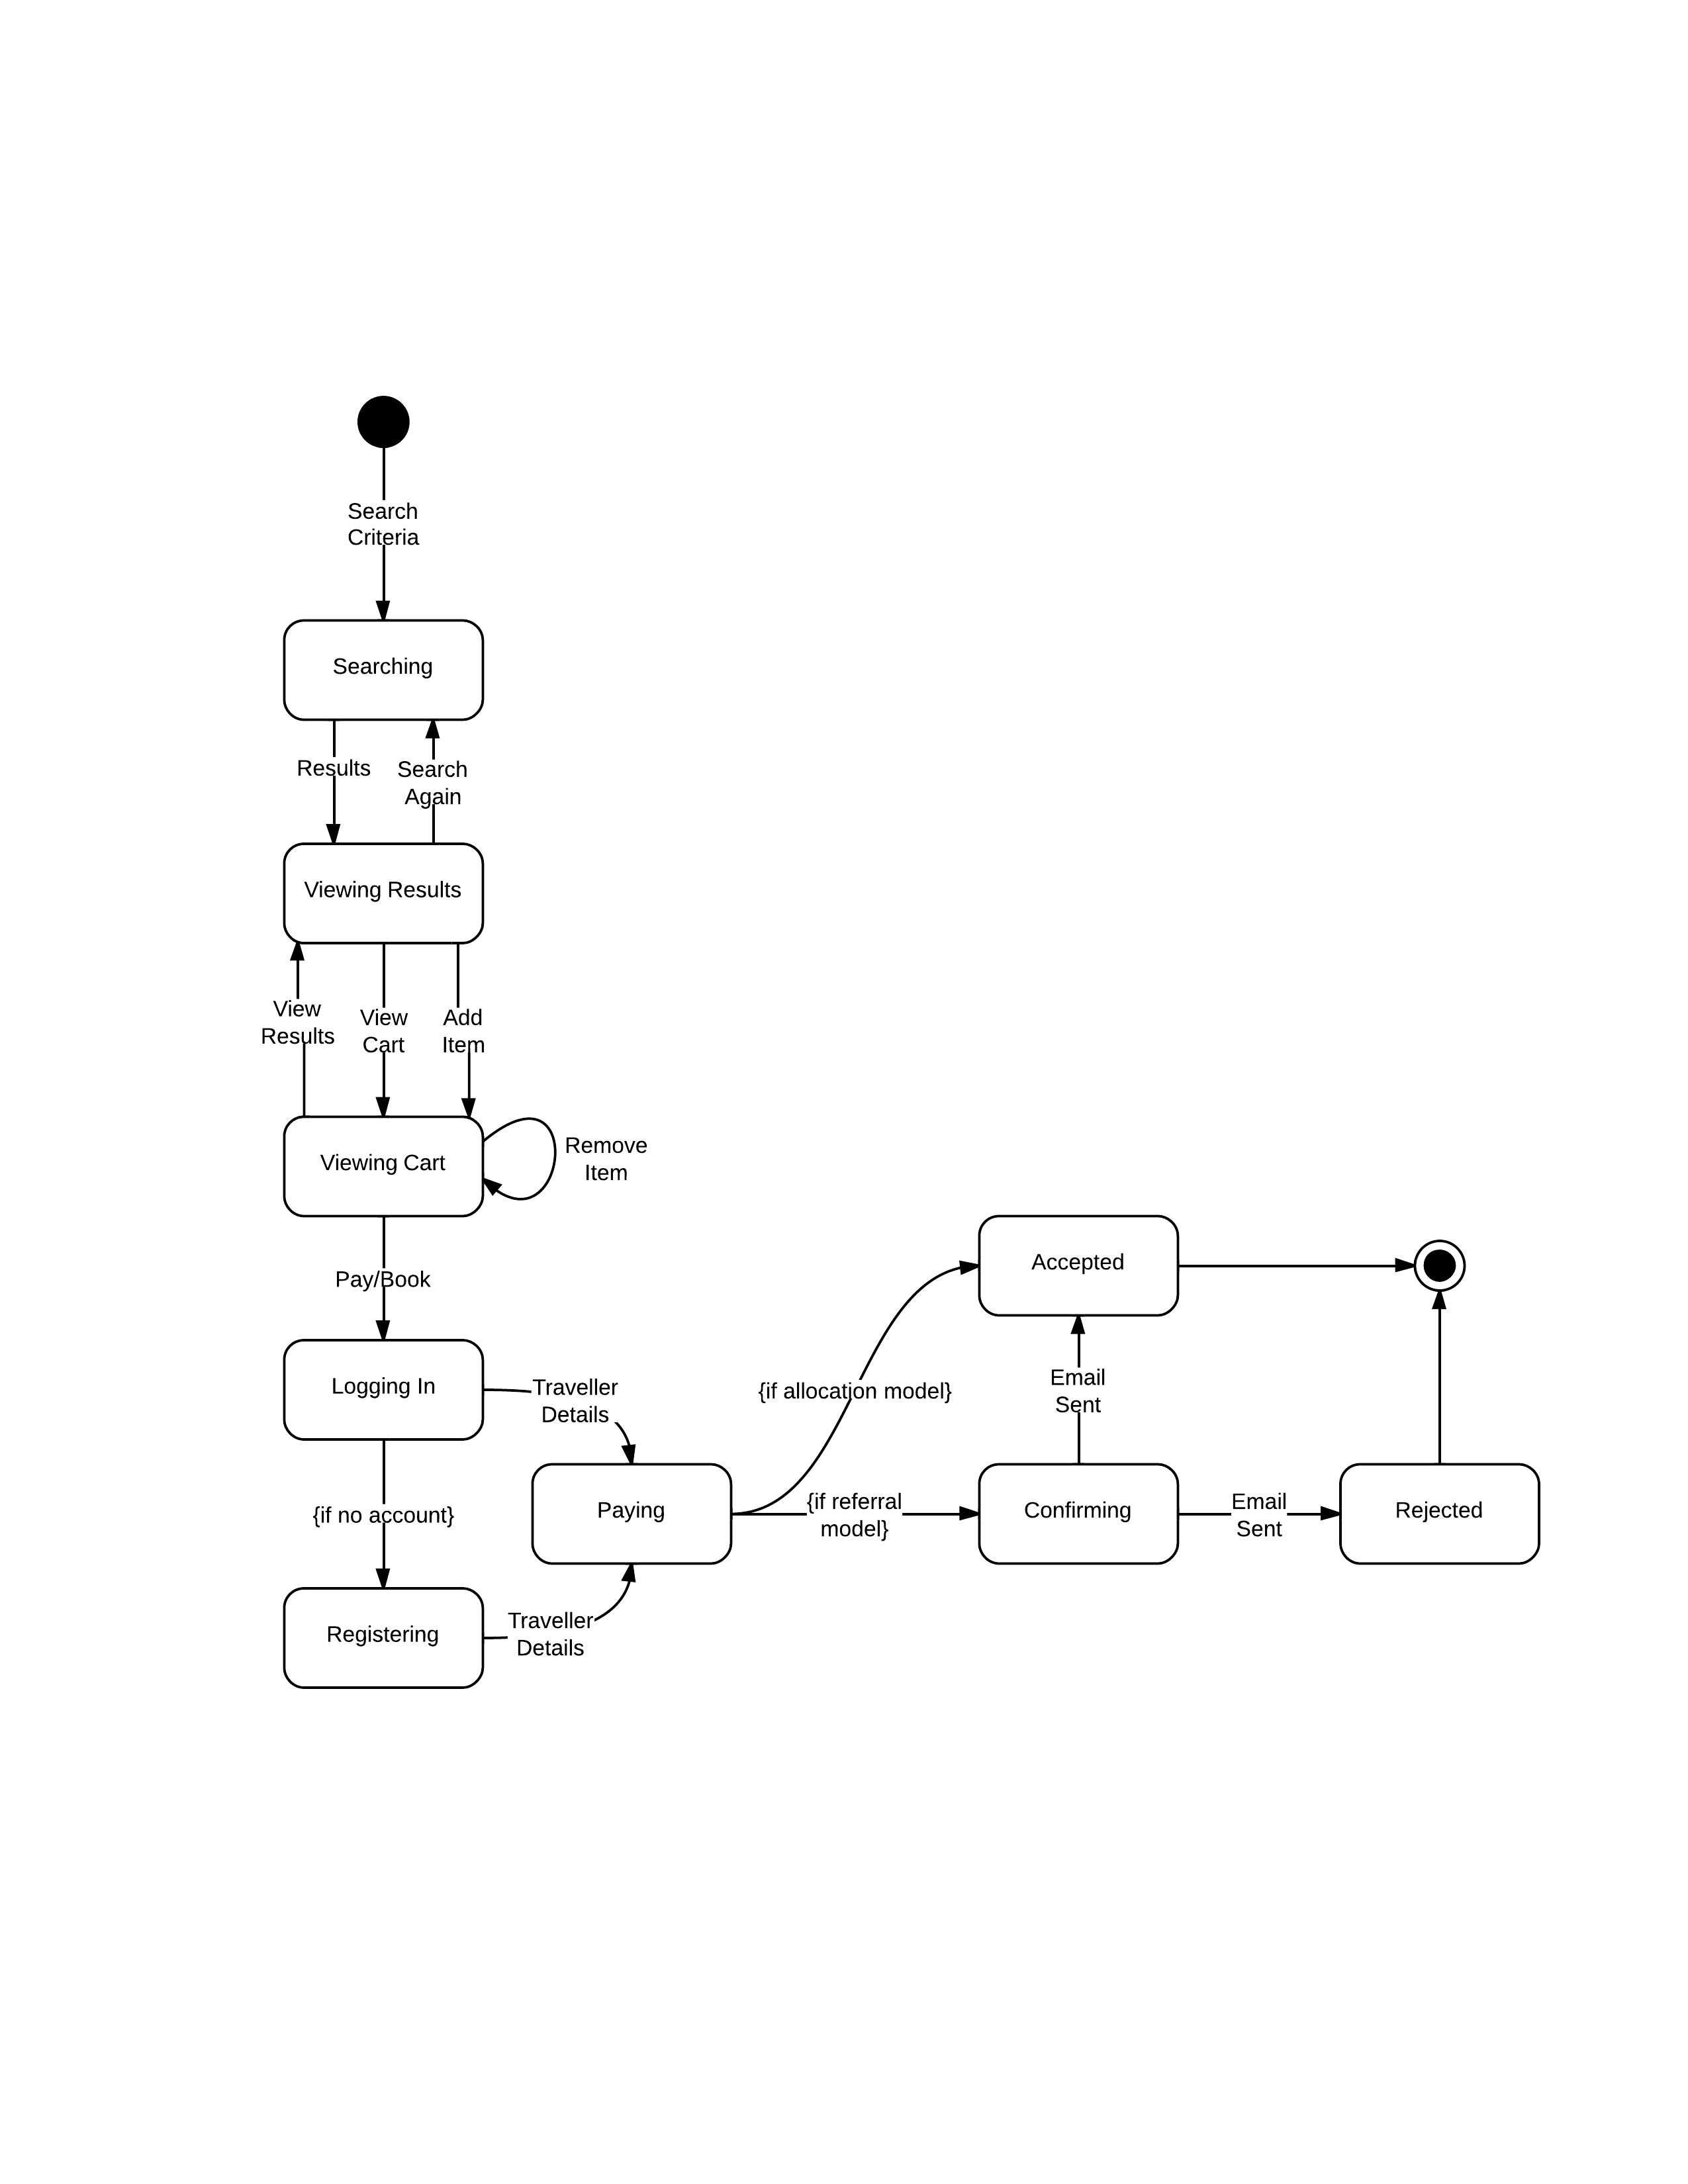
\includegraphics[width=0.7\textwidth]{img/state_diagrams/StateTransitionDiagramUserPayement.png}
\caption{State Transition diagram for Traveller Search, Booking and Payment}
\label{fig:state-traveller-book}
\end{figure}

The final state transition diagram shown in figure \ref{fig:state-traveller-book} shows how a Traveller moves through states in the booking process from initially starting a search through to paying and booking their selected options. Their are several key points in the diagram worth point out. Firstly, note that a Traveller and move freely between searching, viewing results and viewing their cart until they are ready to pay and book. Once they have started down the payment/booking path, they a follow a more linear flow through the system. This was designed to try an emulate a "checkout" feeling of clear operation that need to be performed once the user is comfortable with their choices.

I have also incorporated in the diagram the option for either logging in or going to registering state if the Traveller does bot yet have an account. Note that unlike in figure \ref{fig:state-user-auth} they are not redirected to their account overview, but are returned back into the payment/booking "flow".

Finally, depending on the type of booking model the Hotel is registered with, the Travellers booking will either be automatically accepted (as with the allocation model) or  (in the case of the referral model) the Traveller will move into the "confirming" stage where they will wait until there booking is either confirmed or declined by hotel itself.

\section{Interaction Design}
The next section of this document is concerned with the interaction design for the  Hotel Booking website. This includes a large set of high level wire frame designs for the major pages in the site. In short, this section defines the general structure of the user interface for the website, without real regard for the site's internal operation.

Before going into detail about the design of each of the specific pages, it is first worth talking about features of each page which are consistent across every wireframe. 

Each page is designed to have a banner with the name of the site running across the top of the page, along with a reference to where you are in the site. On the right hand site of the header will be a texbox where a Traveller can perform a "quick search" from anywhere in the site without having to navigate the search page first. There will also be a small section next to this text box indicating where the user is current logged into the system and offering them an option to login/logout accordingly.

Running along the left hand side of the page will be the main navigation section of the site. This will consist of large links for the major areas of the site with sub-links taking the user to specific parts of that section.

In the middle of the screen, below the header and next to the menu is the section of the page which changes according to what page the user is currently on. This section is where new, relevant information will be presented to the user. On most pages, a breadcrumb link will be available to the user to inform them where they currently are and giving the to transcend back up the hierarchy.

\subsection{Traveller Login and Registration}

\begin{figure}[H]
\centering
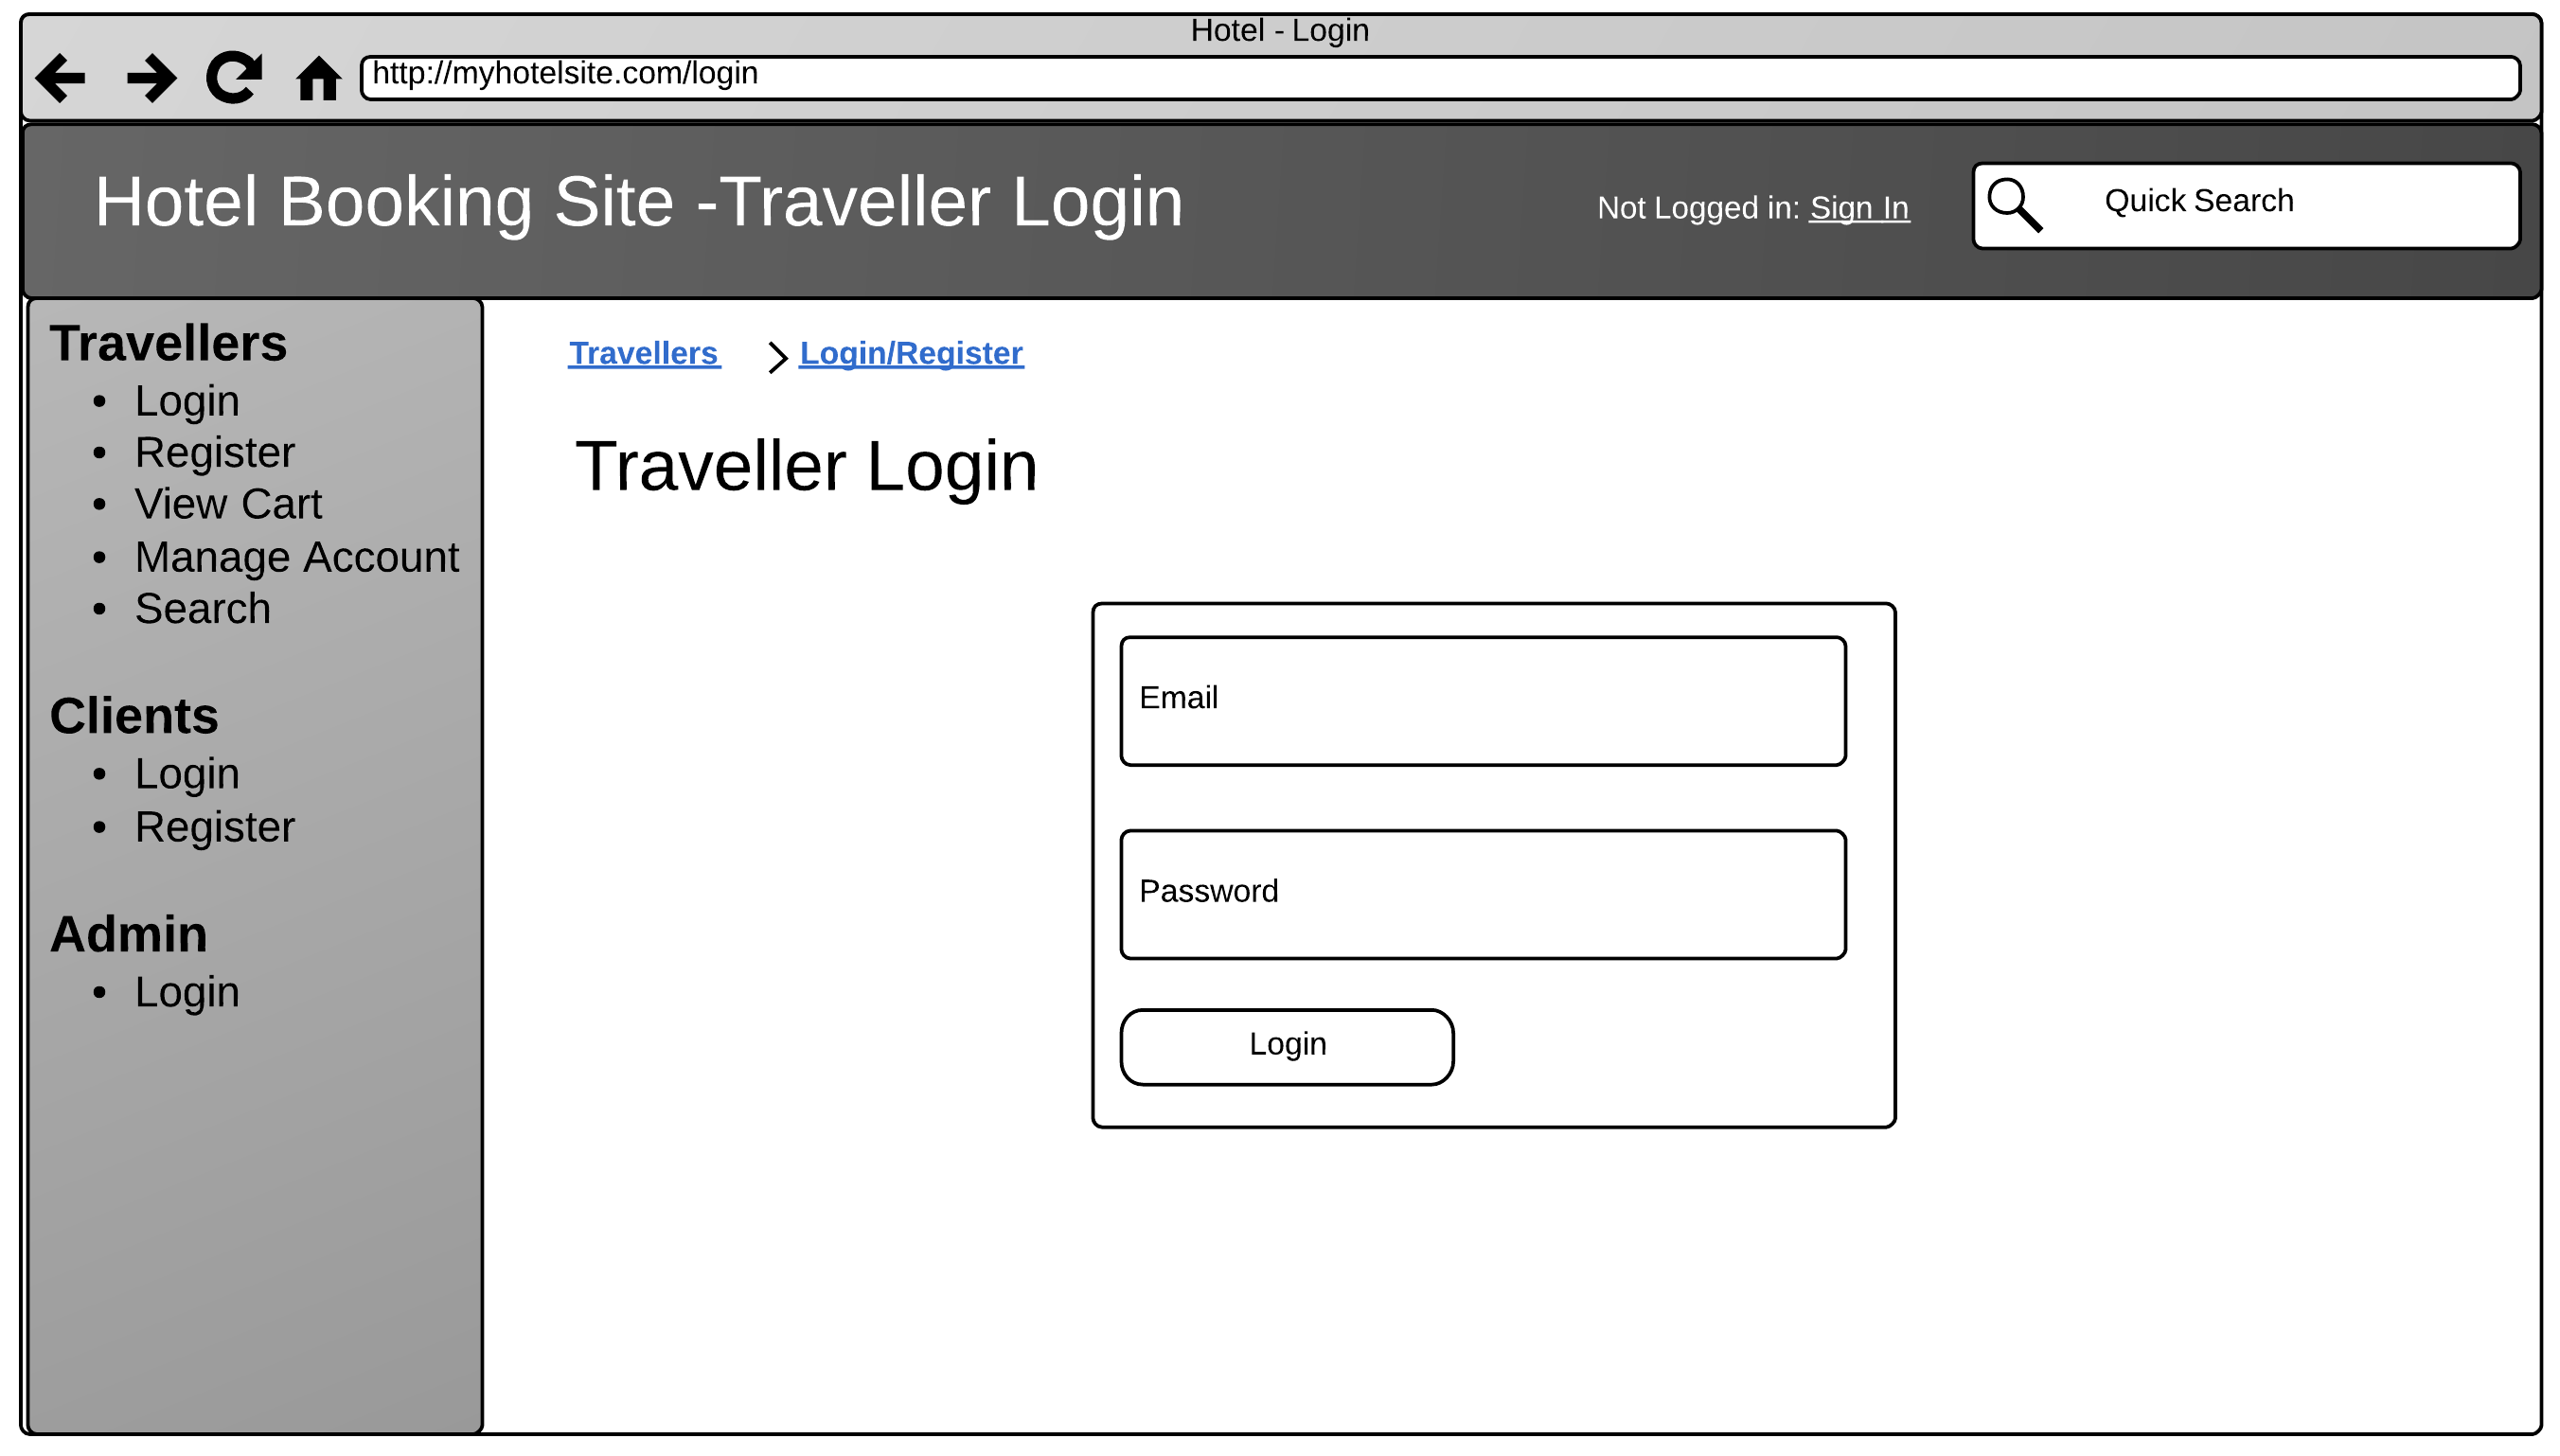
\includegraphics[width=0.7\textwidth]{img/wireframes/Login.png}
\caption{Wireframe for Traveller login page.}
\label{fig:wireframe-traveller-login}
\end{figure}

\begin{figure}[H]
\centering
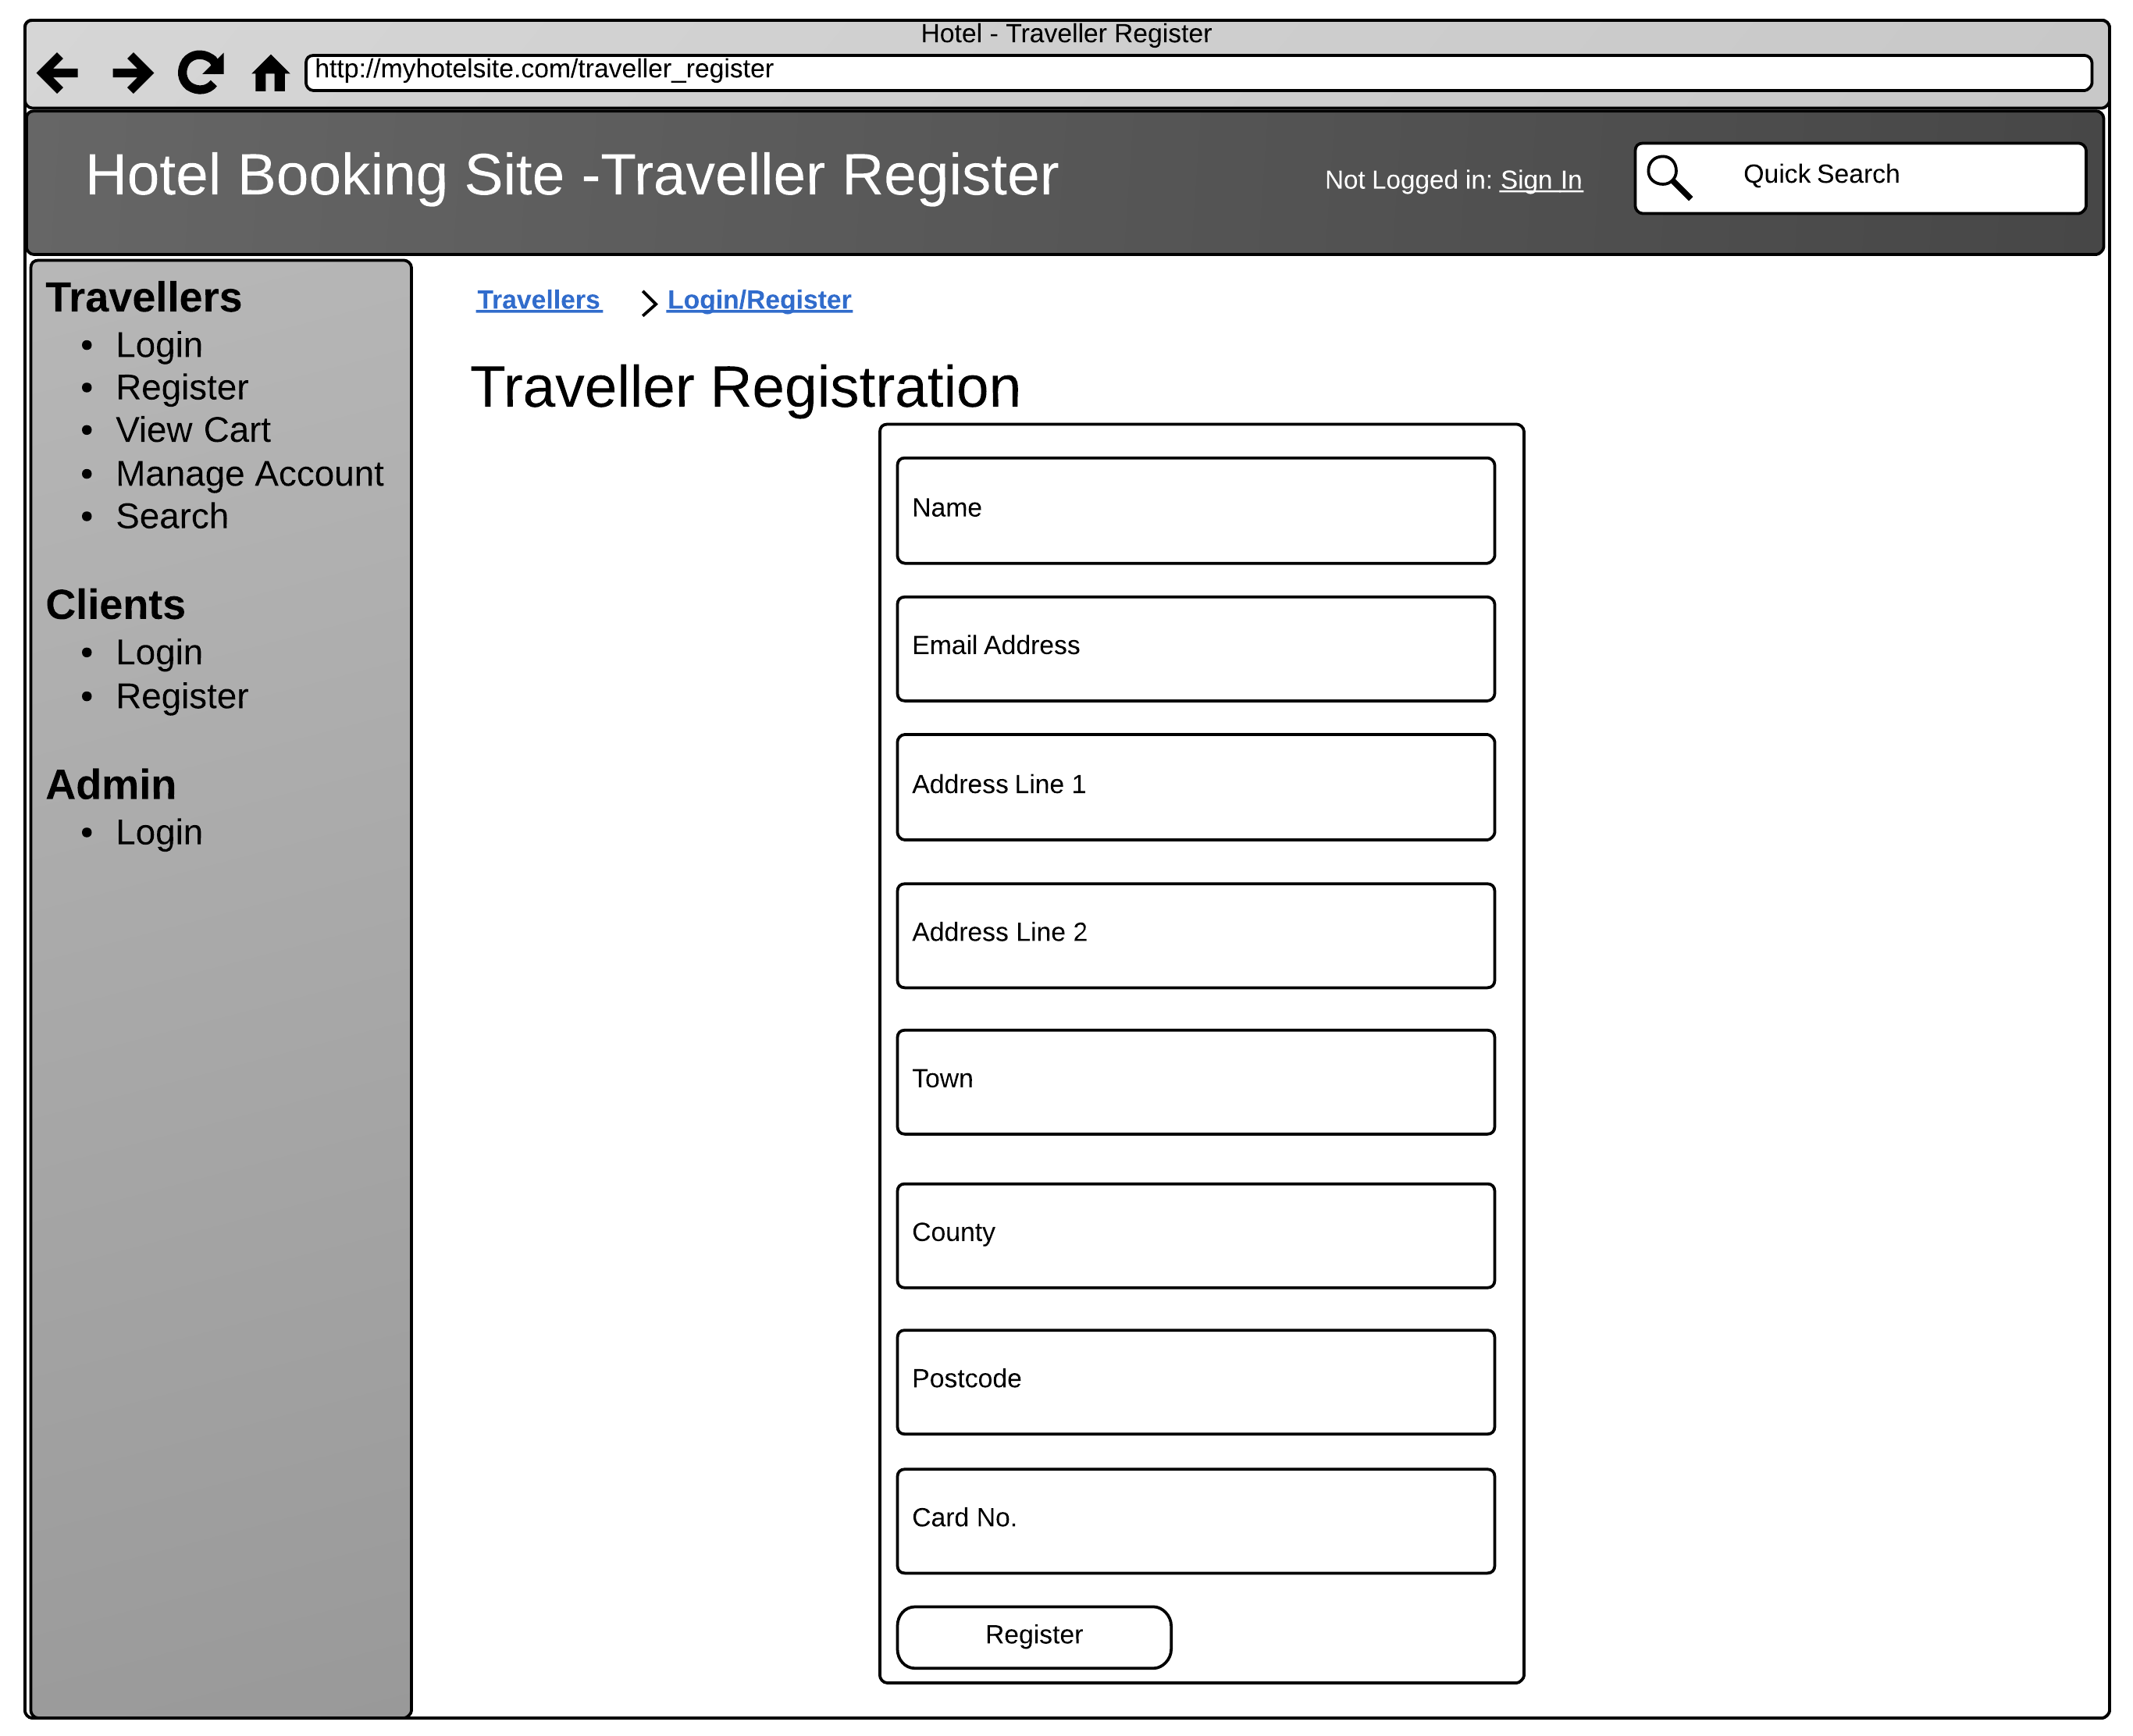
\includegraphics[width=0.7\textwidth]{img/wireframes/TravellerRegistration.png}
\caption{Wireframe for Traveller registration page.}
\label{fig:wireframe-traveller-register}
\end{figure}

The first to wireframes show an overview of the design of the Traveller login and registration pages. Both of these page use a straight forward design, clearly displaying a form with a label identifying what input is expected in each field. At the bottom of each of the forms is a button of the user to submit the action to server. Again this is clearly labelled to tell the user exactly what action they will be performing when clicking it.

\subsection{Client Login and Registration}

\begin{figure}[H]
\centering
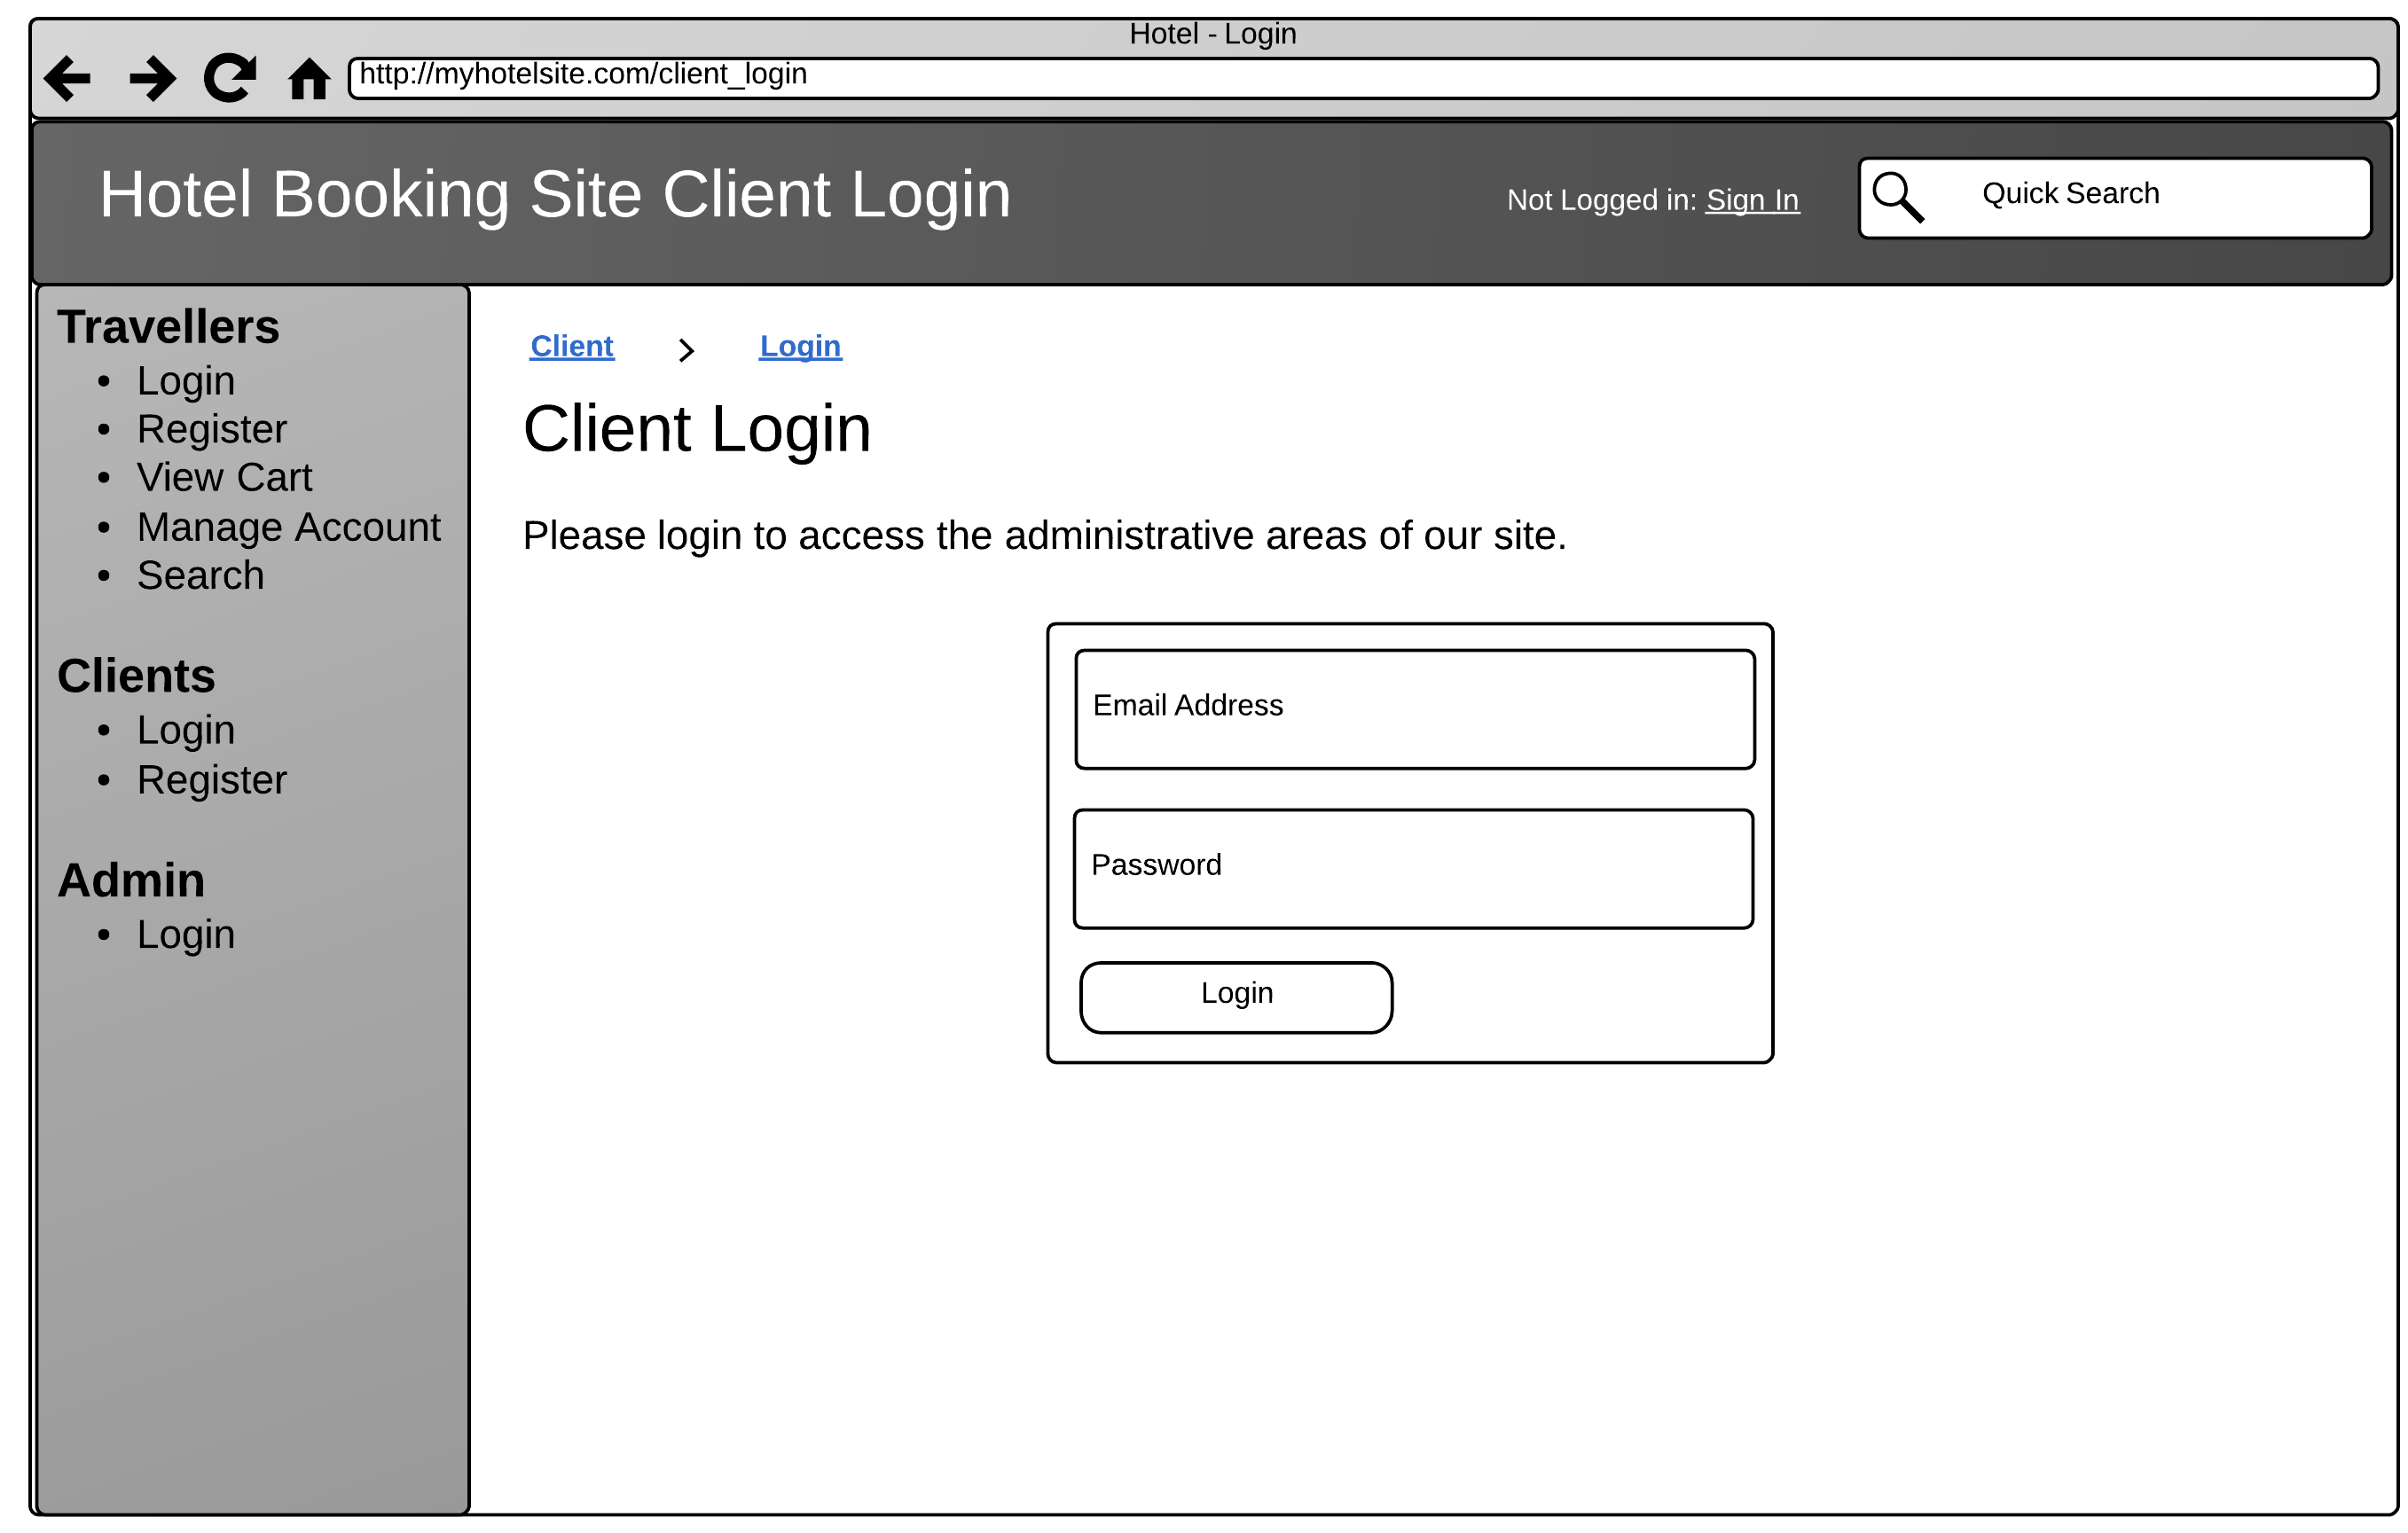
\includegraphics[width=0.7\textwidth]{img/wireframes/ClientLogin.png}
\caption{Wireframe for Client login page.}
\label{fig:wireframe-client-login}
\end{figure}

\begin{figure}[H]
\centering
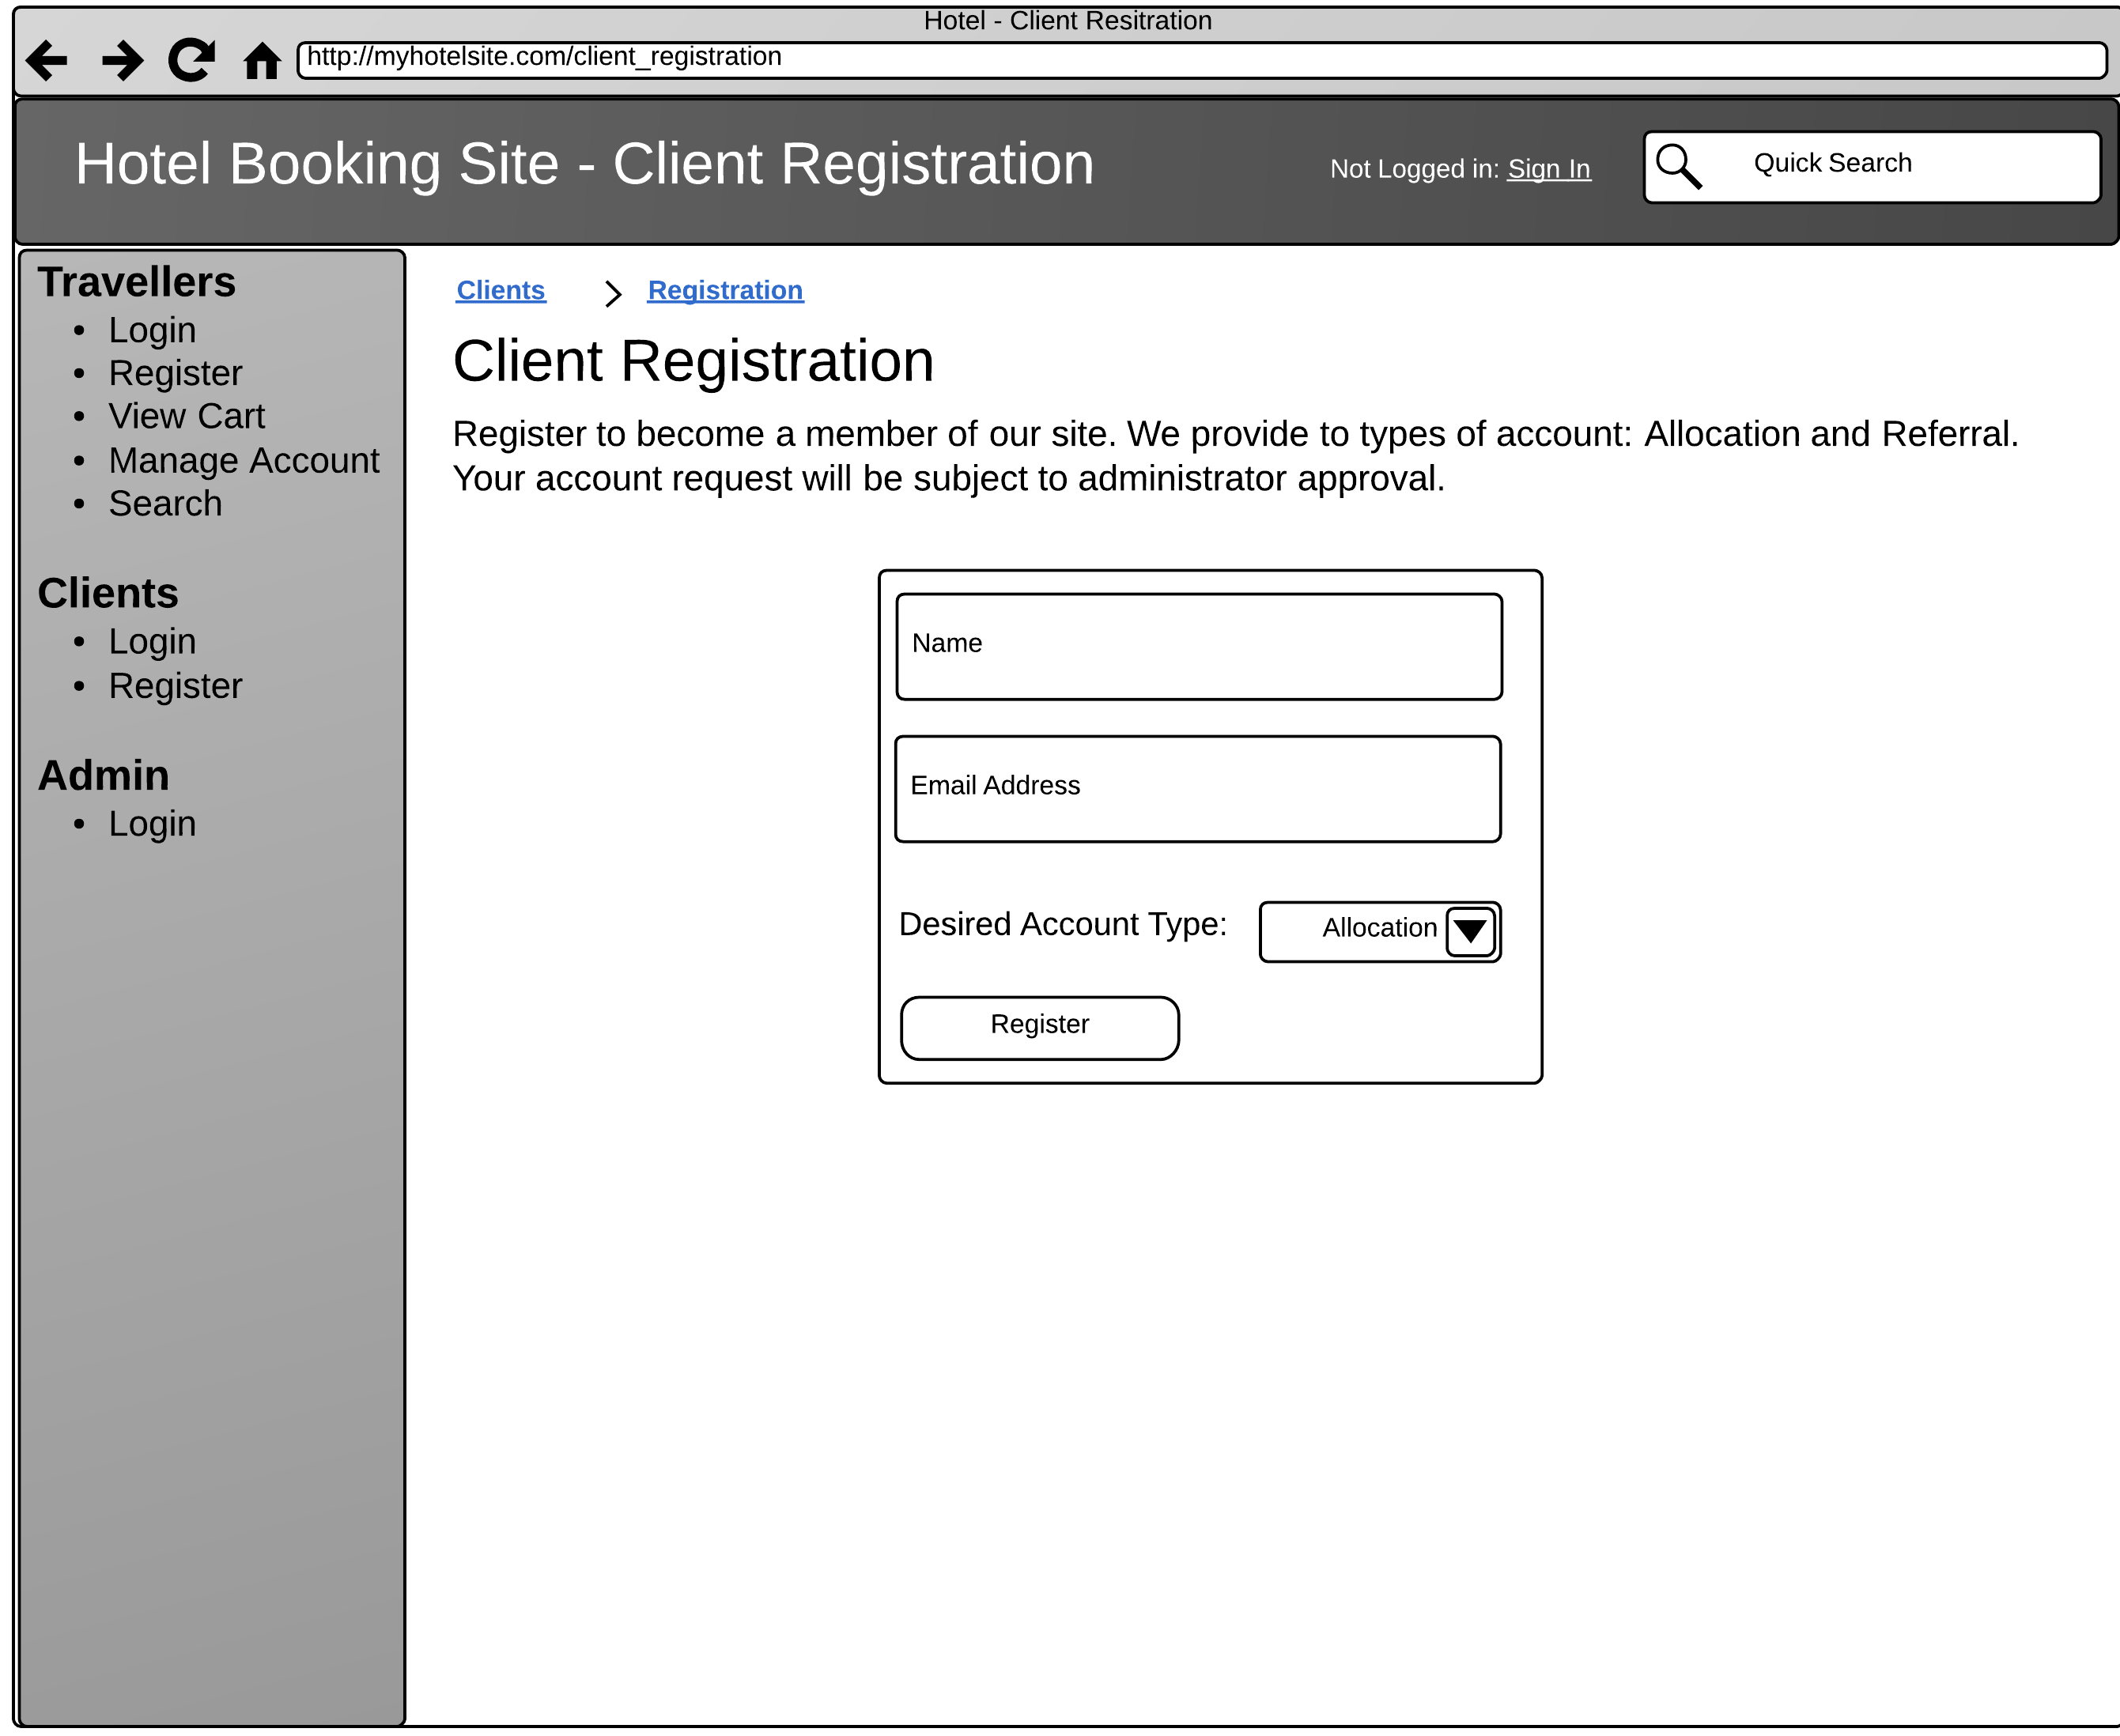
\includegraphics[width=0.7\textwidth]{img/wireframes/ClientRegister.png}
\caption{Wireframe for Client registration page.}
\label{fig:wireframe-client-register}
\end{figure}

The next two wireframes show the designs for the Client login and registration pages and a quite similar to the traveller login and registration pages, except that registration requires different fields. I have chosen to use a drop down menu for account type so as the clearly limit the options available to the user. Information about the what the types of model could be described in brief at the top of the page and possible in further detail on a help page. In actual development, when a client chooses which model they would like to apply for, if the allocation model is selected, I would expect an additional field to allow the user to input how many rooms they would like to be allocated to there account.

Unlike a Traveller, when a Client clicks to register with the Hotel Booking site, they are not taken directly to view their account overview. Instead, because a site administrator needs to approve the request for registration, they are shown the "pending registration" page, informing them that they will be notified by email if their request is accepted or declined.

\begin{figure}[H]
\centering
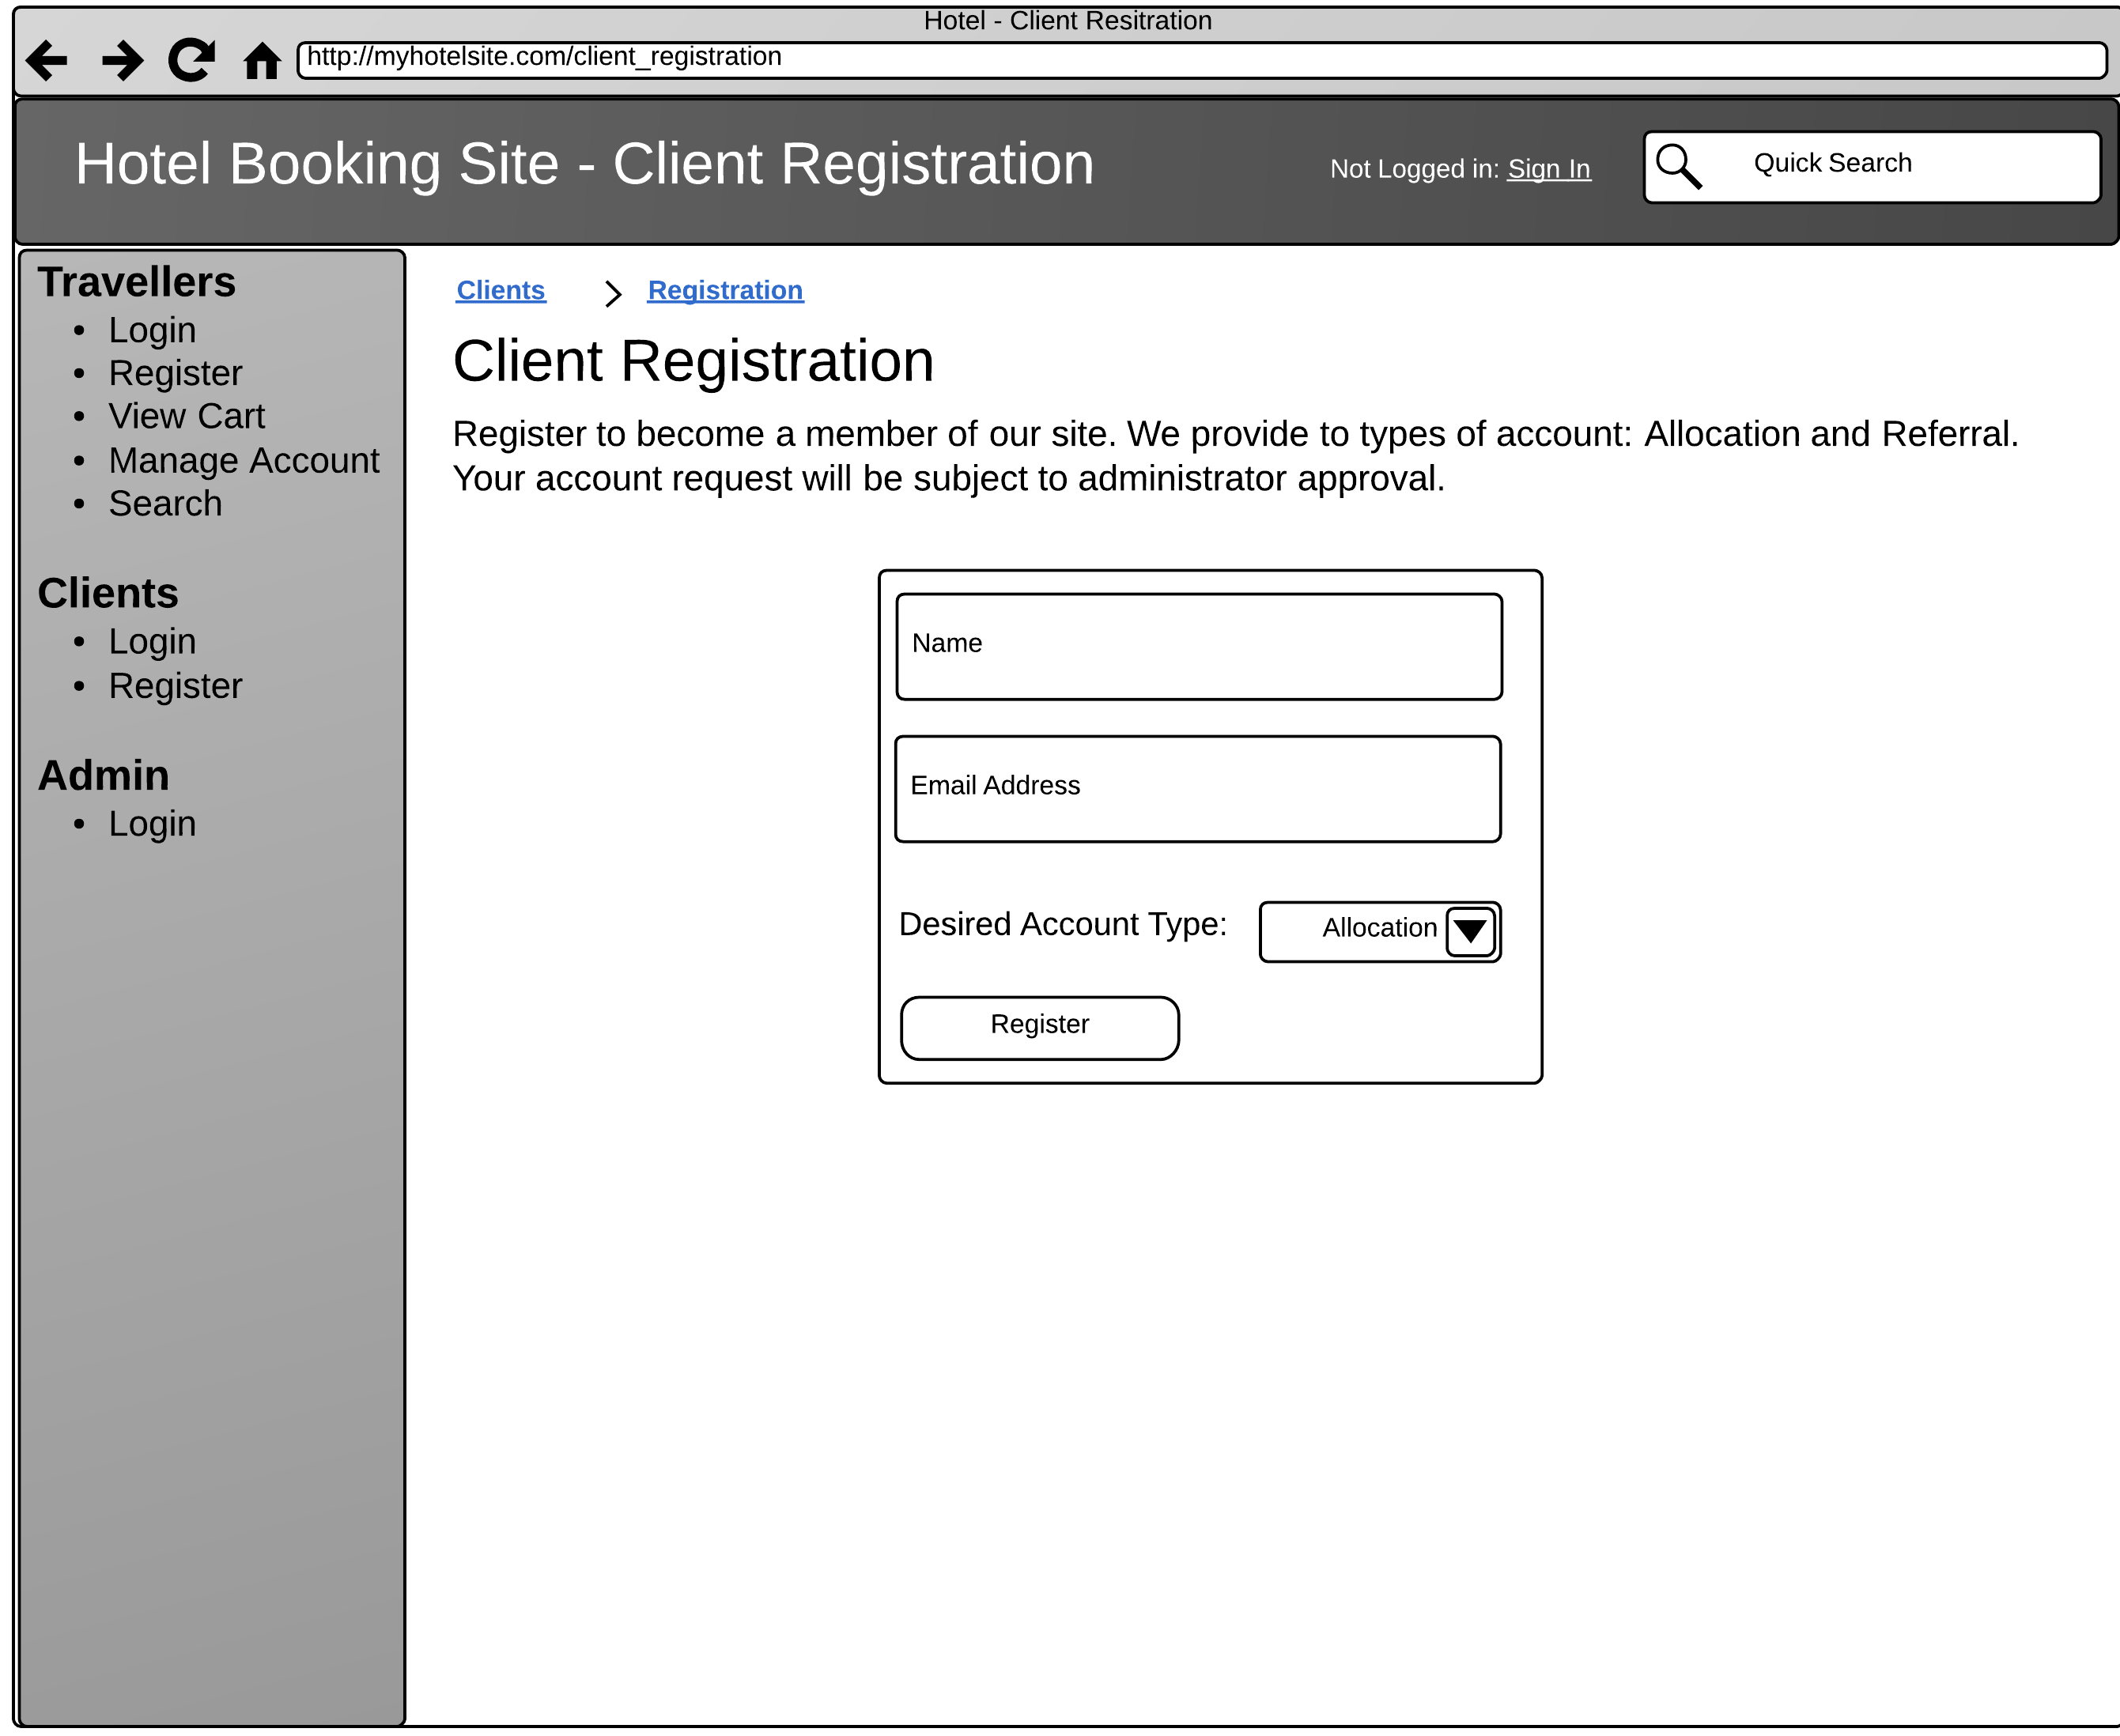
\includegraphics[width=0.7\textwidth]{img/wireframes/ClientRegister.png}
\caption{Wireframe for Client registration page.}
\label{fig:wireframe-client-register}
\end{figure}

\subsection{Administrator Login}
The next wireframe for the administrator login follows suit of the other two, simply requiring the user to enter an email address and password to again access to their account. Note that administrators do not have a page for registration. It is assumed that they are allocated an account with the hotel booking site either through the site's server administration or by some other system.

\begin{figure}[H]
\centering
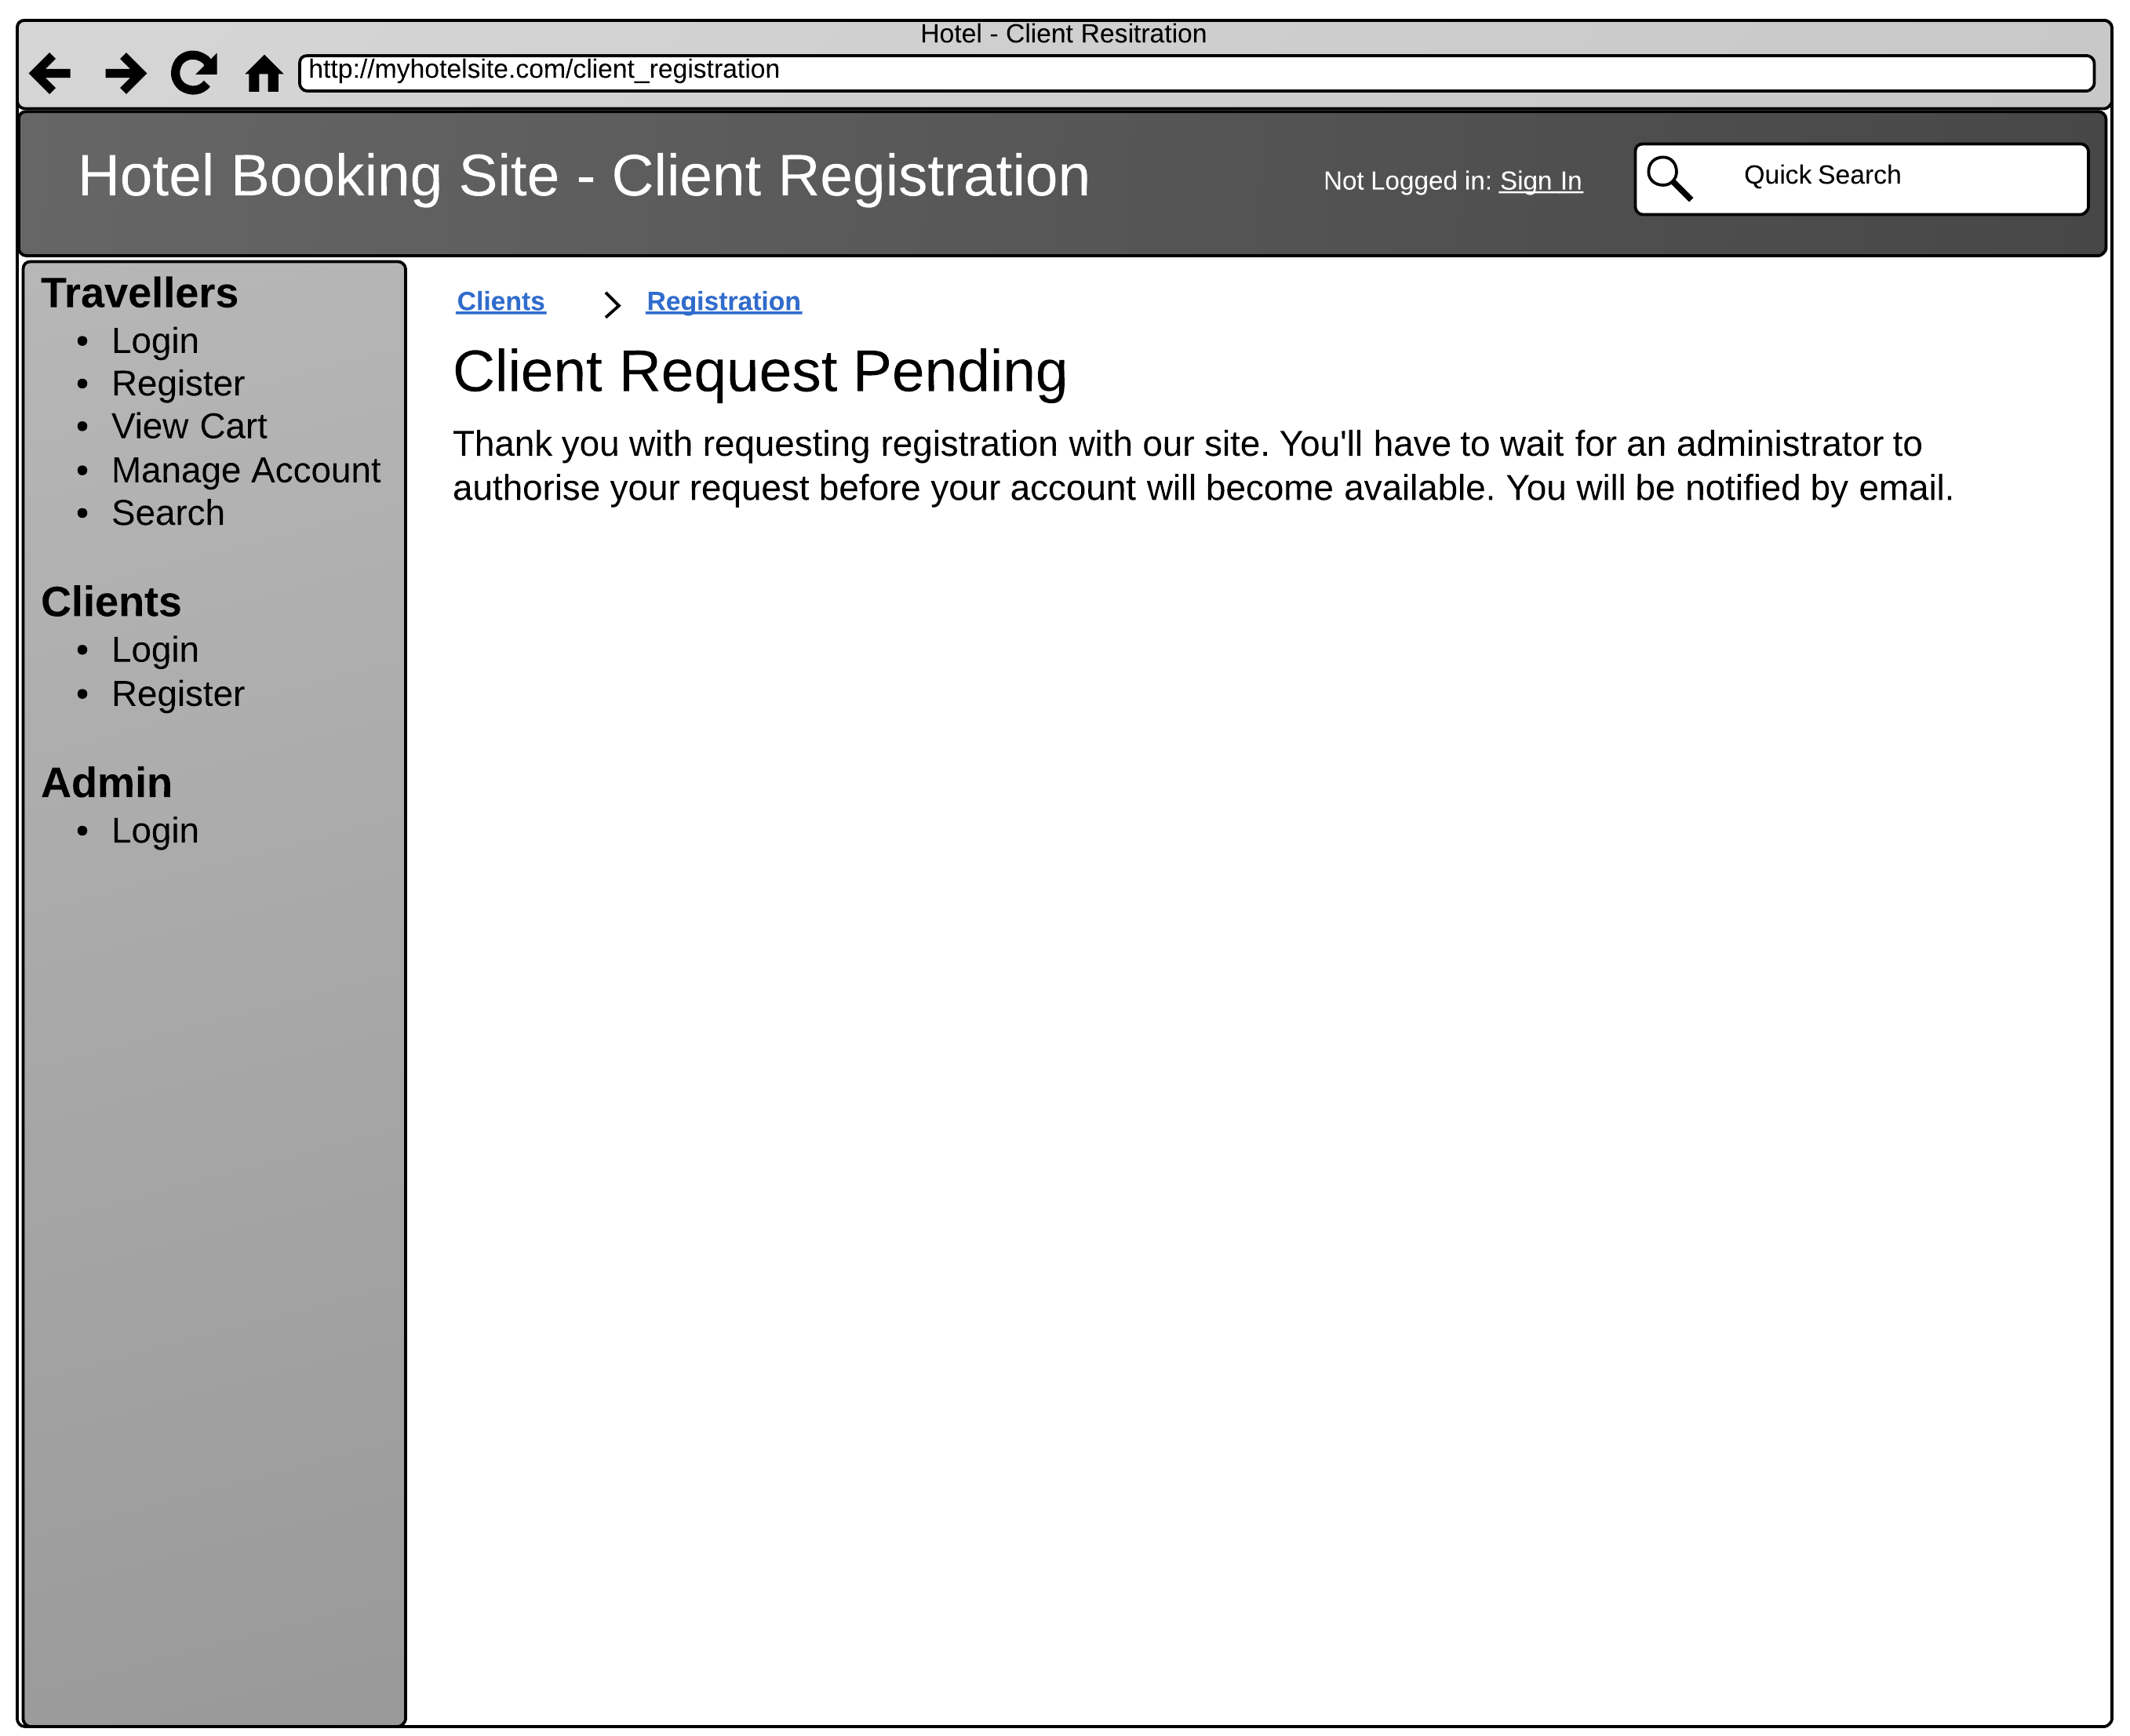
\includegraphics[width=0.7\textwidth]{img/wireframes/ClientPending.png}
\caption{Wireframe for the Client registration pending page.}
\label{fig:wireframe-client-pending}
\end{figure}

\subsection{Traveller Account Management}
This wireframe shows the design for the travellers account management page. Like most pages, this design incorporates the name of the traveller at the top of the page just below the breadcrumb navigation element. It also contains a simple textual description of about what the user do on this page. The rest of the page is split into to forms separated by a field-set. The first form allows of editing the users billing address and the second allows for editing the payment card they have registered with their account.

\begin{figure}[H]
\centering
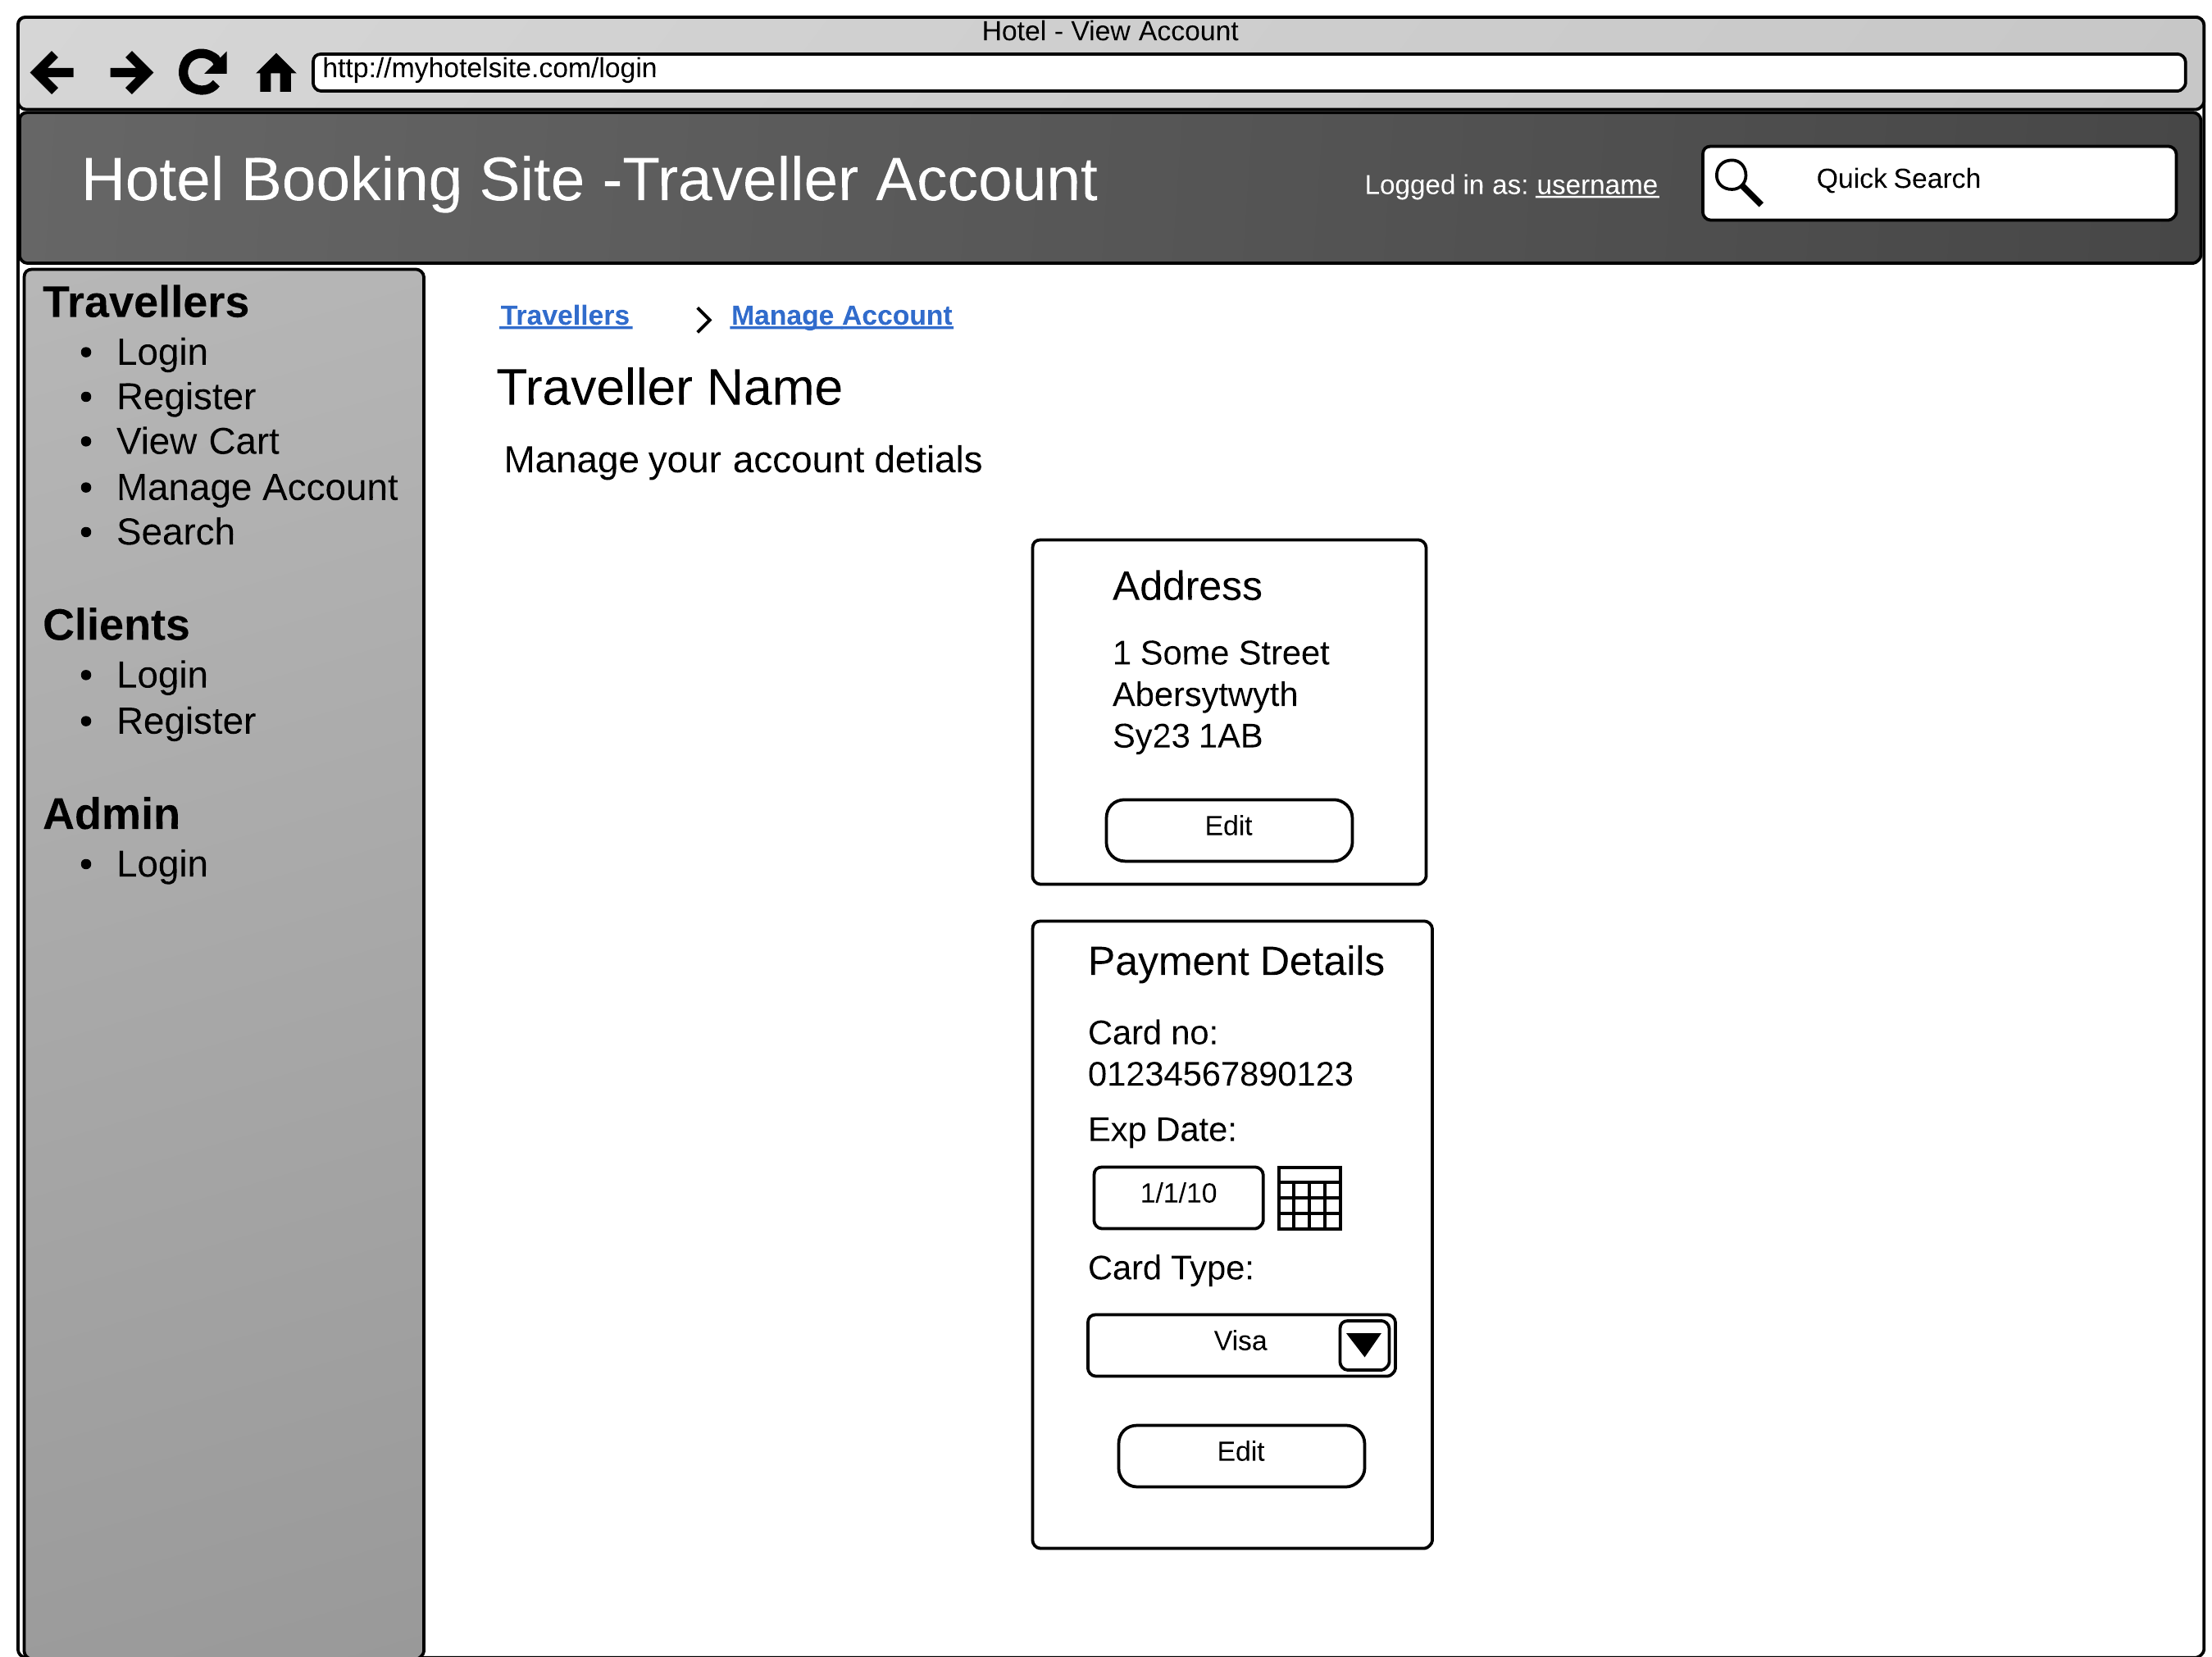
\includegraphics[width=0.7\textwidth]{img/wireframes/TravellerAccount.png}
\caption{Wireframe for Traveller management page.}
\label{fig:wireframe-client-register}
\end{figure}

\subsection{Client Account Management}
This section shows the collection of interface designs for the Client management facilities available on the site. Client management is the most complex part of the management system. The first wireframe design shown in figure \ref{fig:wireframe-client-management} shows entry point the user is shown when accessing Client management facilities. This wireframe is equivilent to the "Viewing Account Overview" state shown in figure \ref{fig:state-client-manage}.

Figure \ref{fig:wireframe-client-management} shows the full version of the Client account management interface, i.e. the one which the comes with an allocation account. If the Client was assigned a referral account, the only feature that would bes displayed to them would be the ability to edit the promotional information at the top half of the page.
 
\begin{figure}[H]
\centering
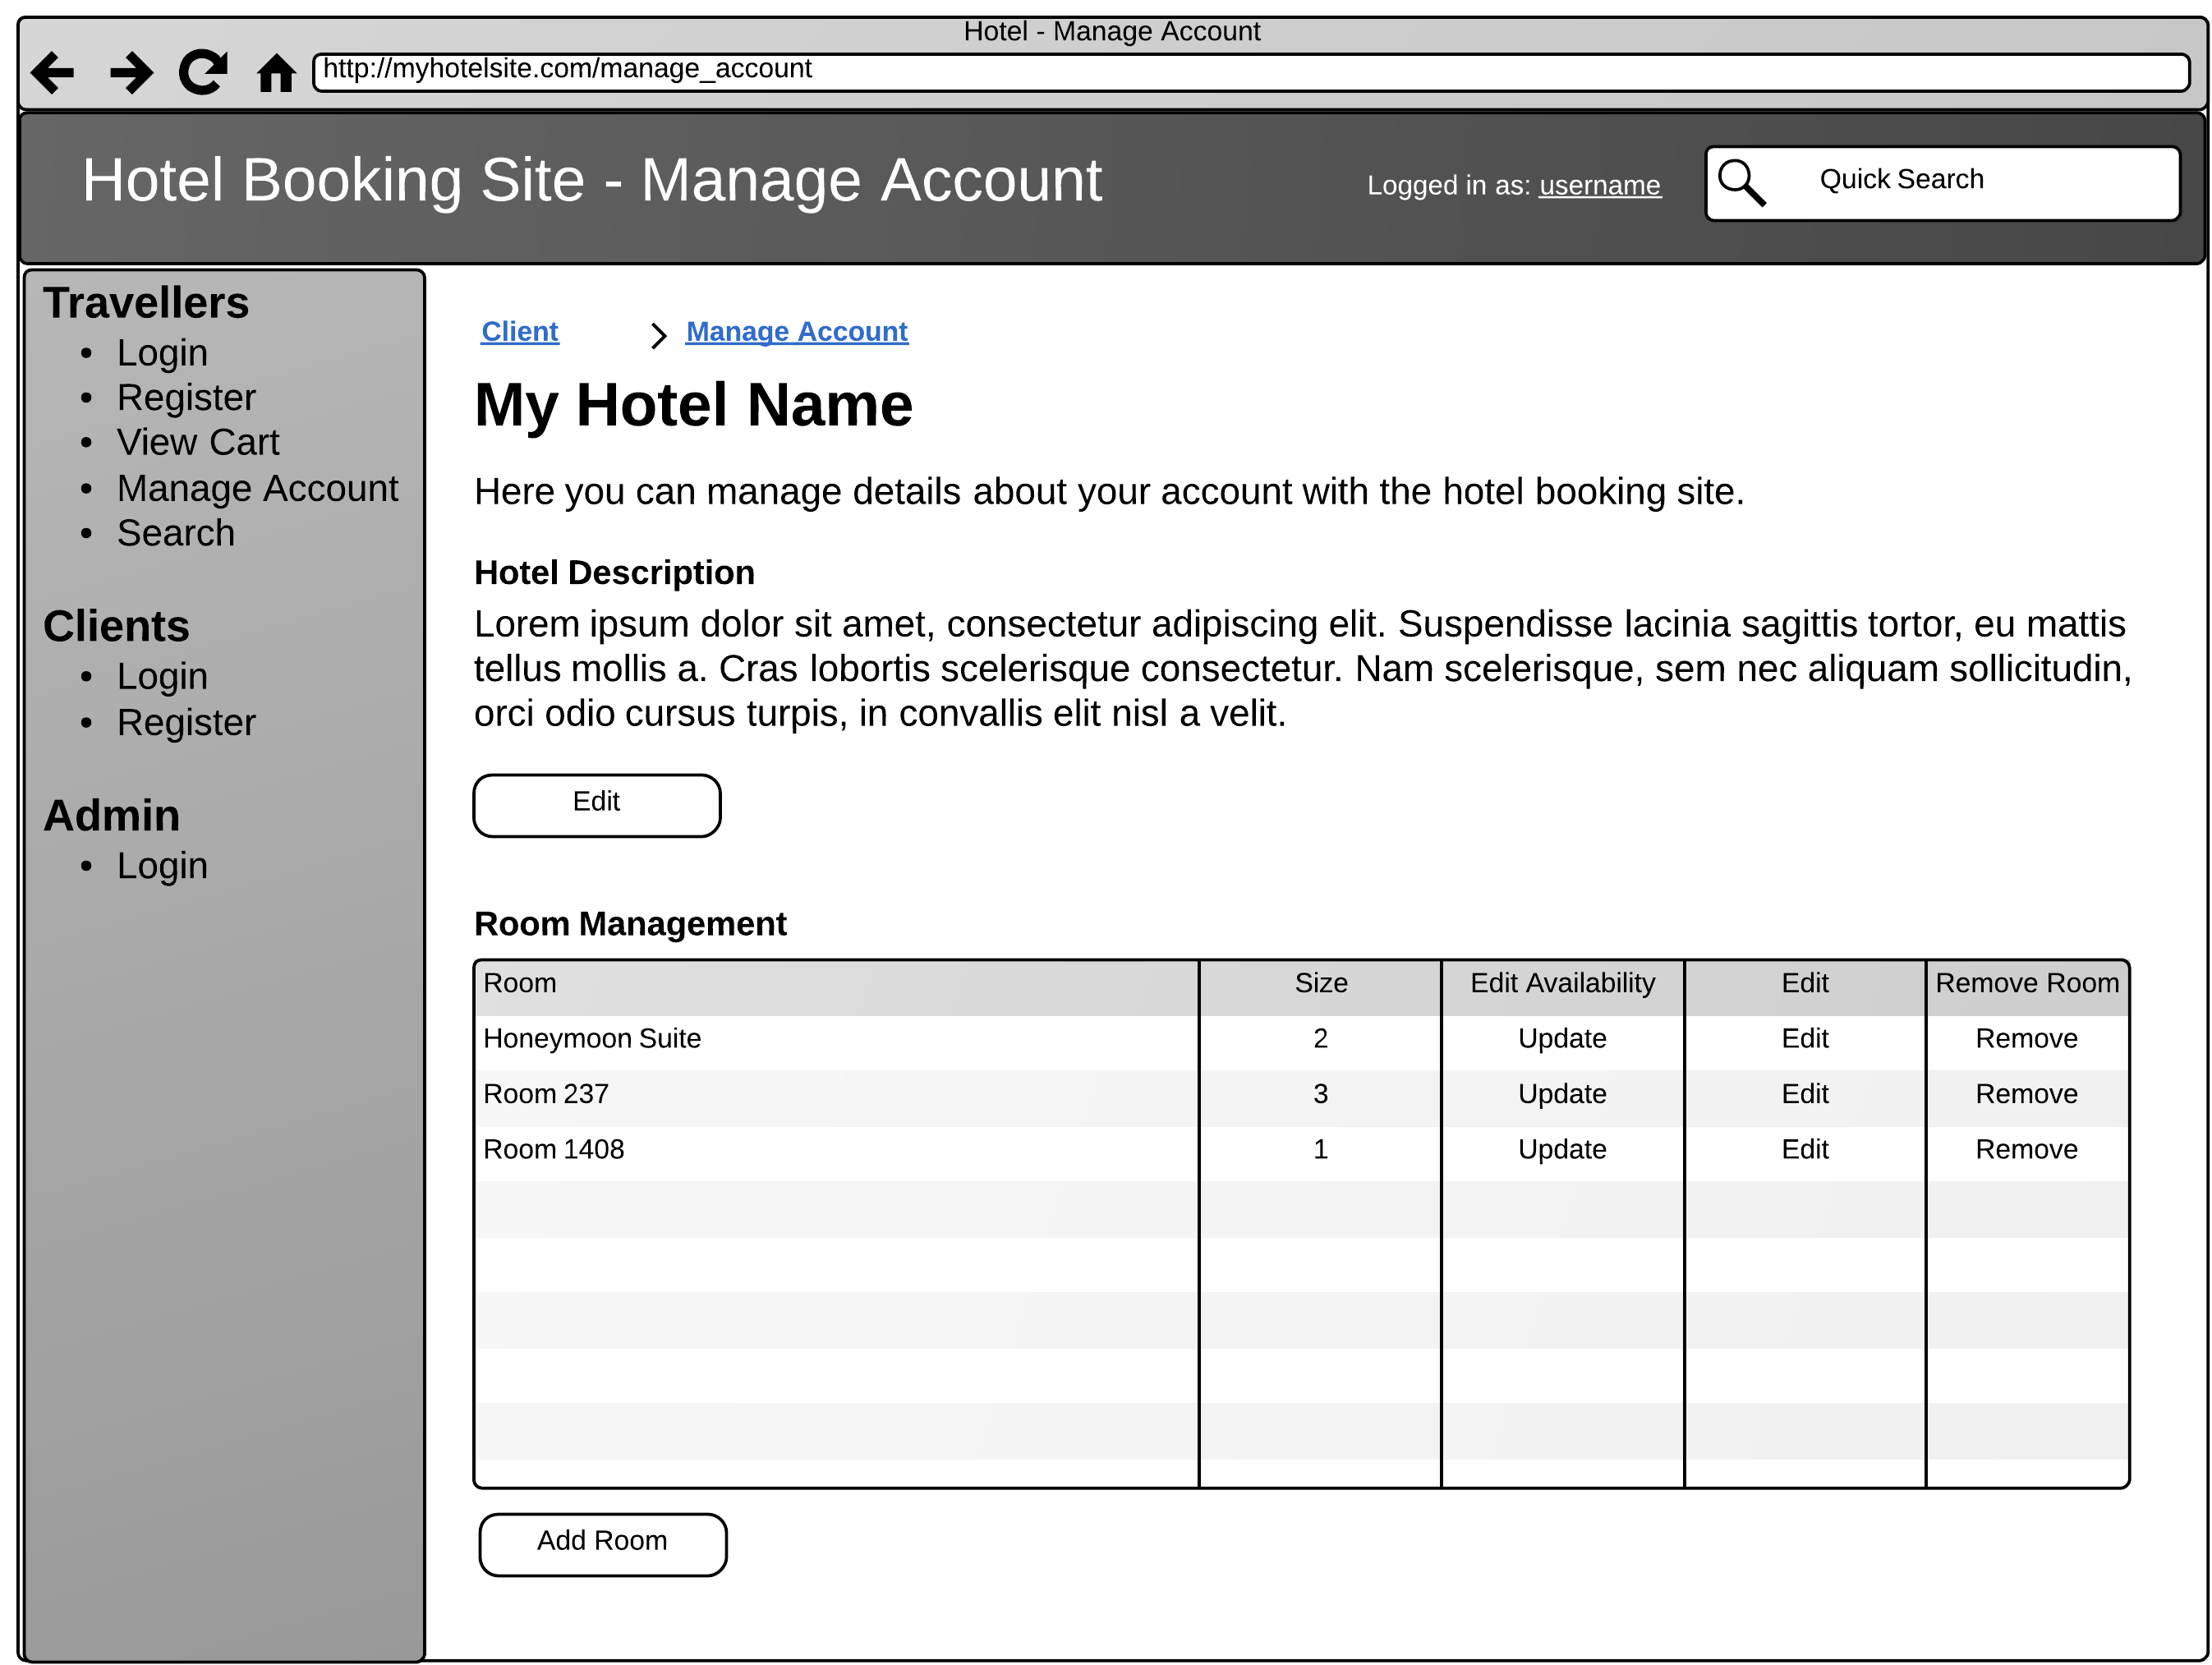
\includegraphics[width=0.7\textwidth]{img/wireframes/ClientManagement.png}
\caption{Wireframe for Client management page.}
\label{fig:wireframe-client-management}
\end{figure}

The bottom half of the page shows the design for the interface allowing the Client to add, remove, edit and update the availability of the rooms they have listed on the site. I have decided that the most clear and user friendly way of displaying this data and the available actions associated with it would be to show it in tabular form with clear headings for each column. This seemed sensible as it allowed me to clearly convey a large amount of data to the user in a relatively compact space. Again, like previous forms, the actions available to the user will shown in the form of clearly labelled, click-able buttons.

\begin{figure}[H]
\centering
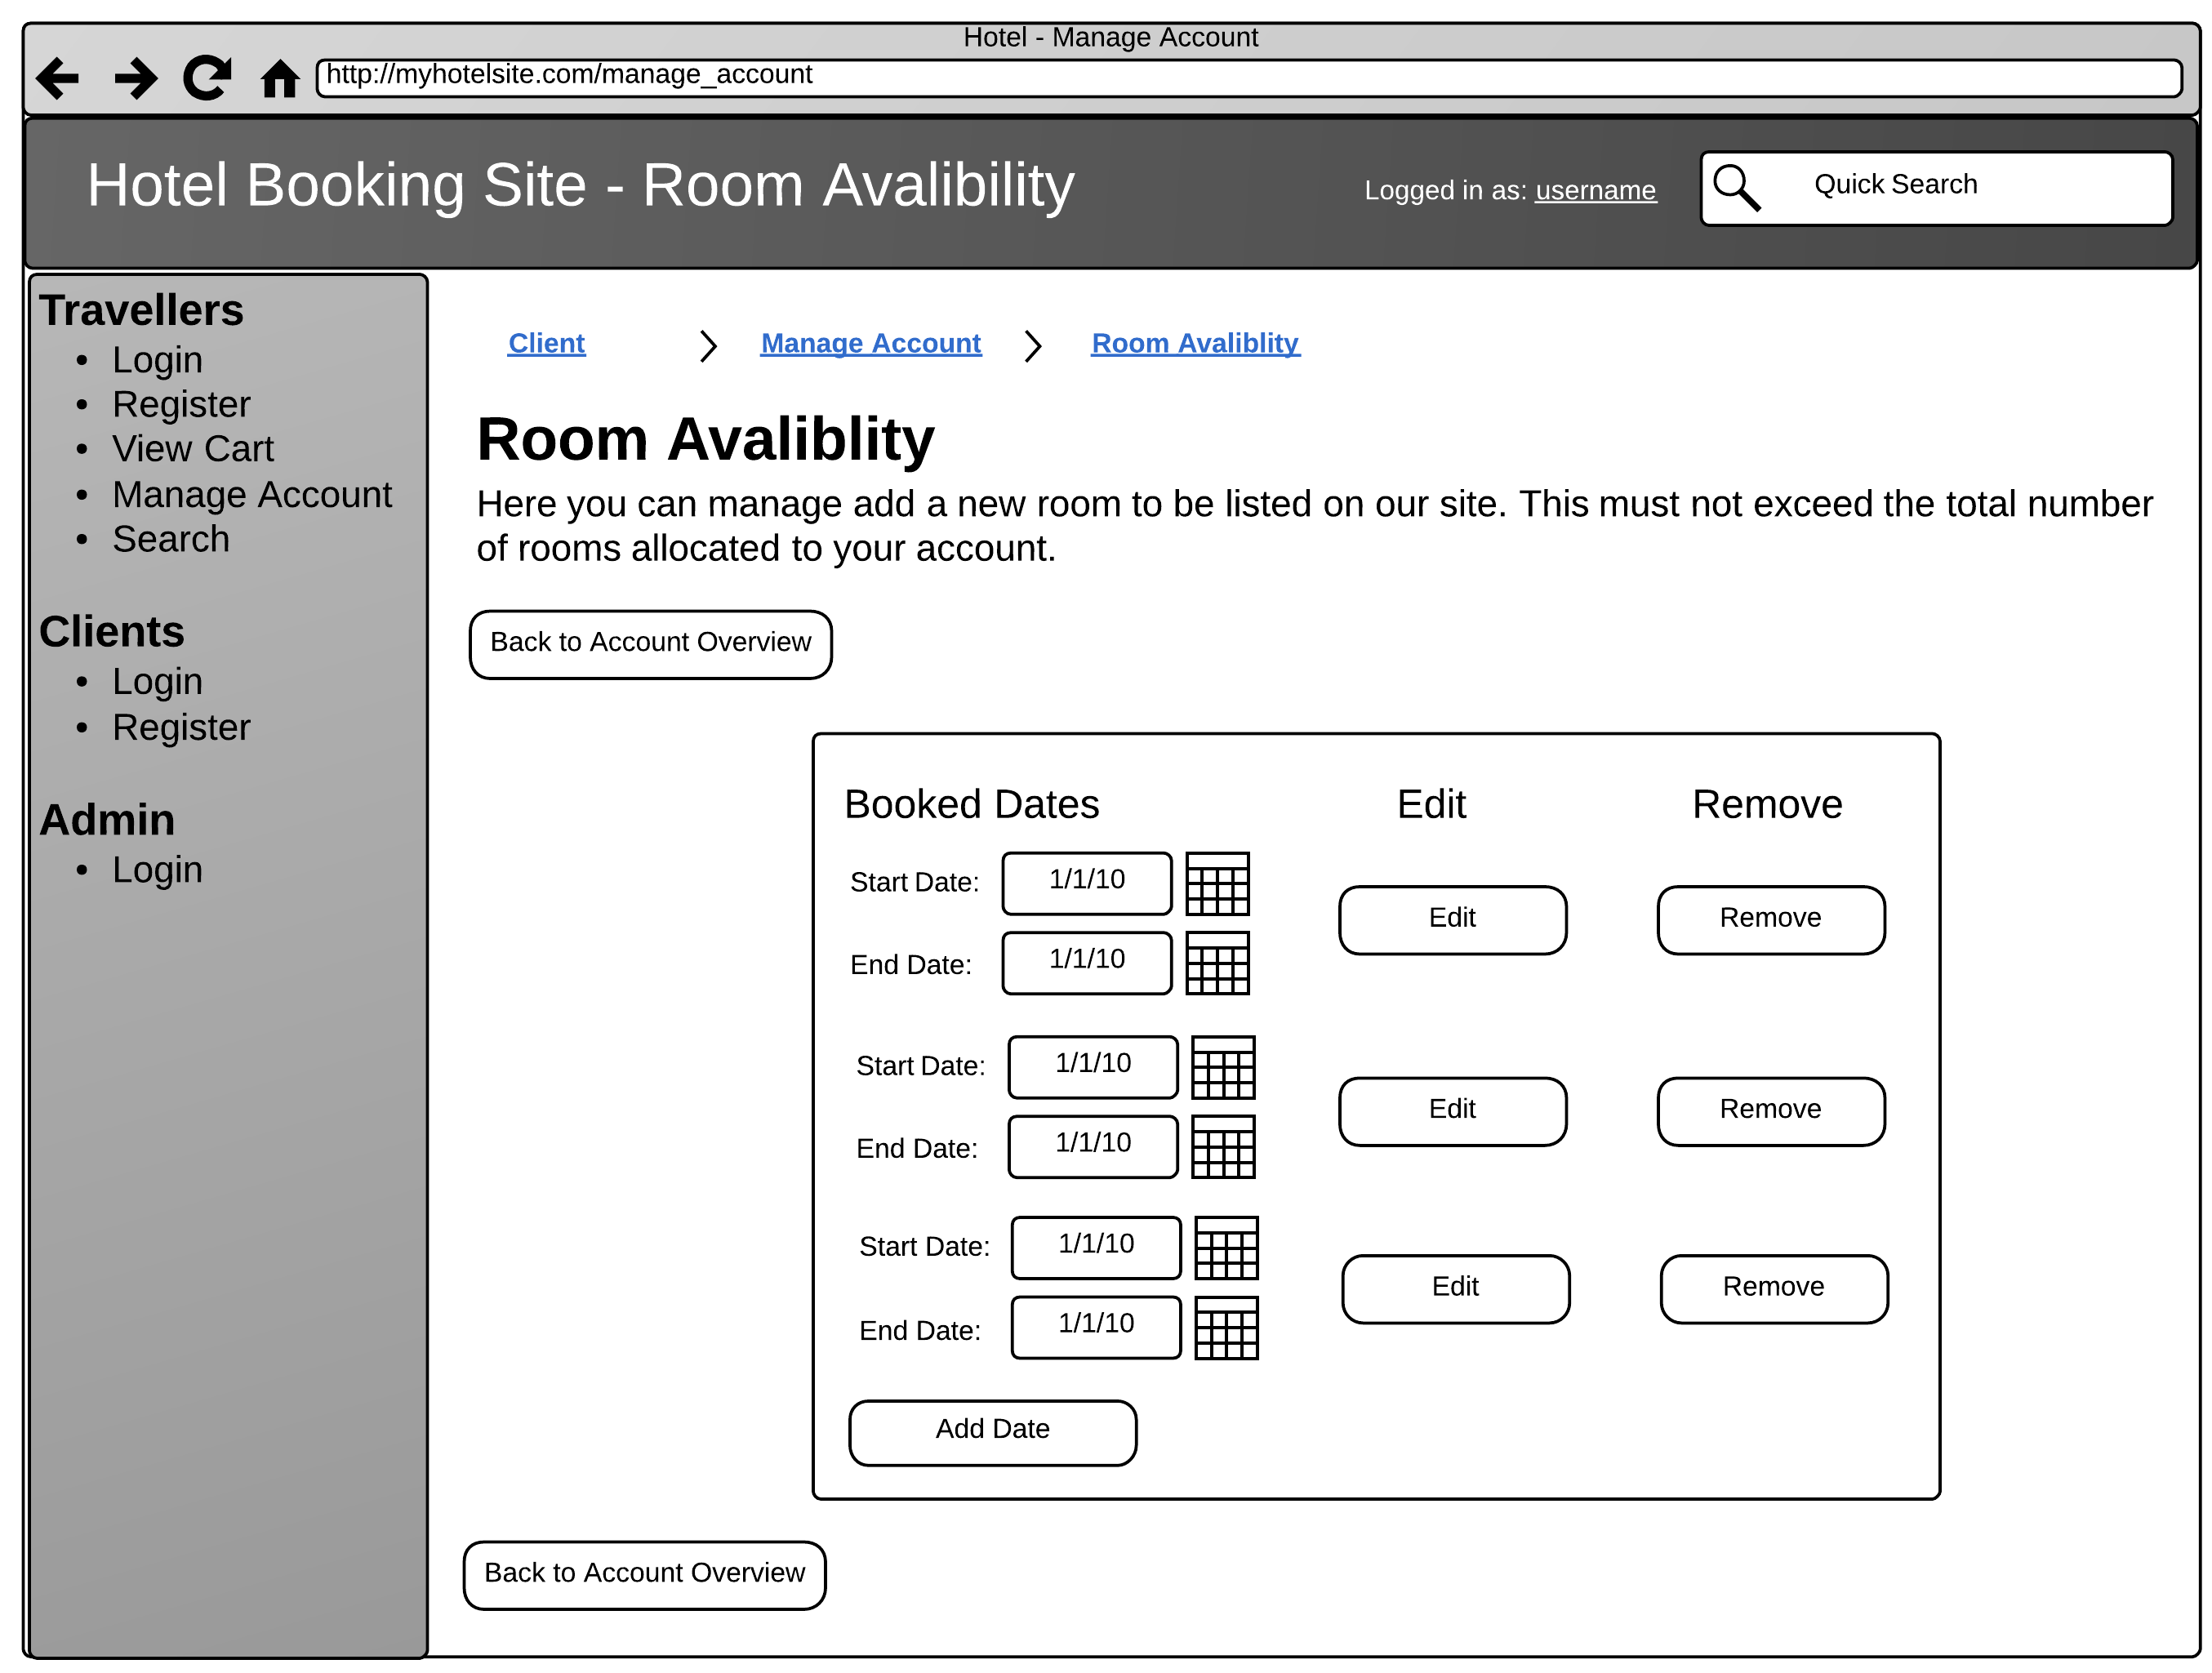
\includegraphics[width=0.7\textwidth]{img/wireframes/EditAvalibility.png}
\caption{Wireframe for editing the availability of a room.}
\label{fig:wireframe-client-availability}
\end{figure}

The next wireframe, figure \ref{fig:wireframe-client-availability} shows the screen for editing the availability of a room. This option is reached by clicking on the "Update" button shown in figure \ref{fig:wireframe-client-management}. Similarly, I have chosen to display the data about each of the dates the room is booked for in tabular format for the same reasons.

Also note that this page has an option to return to the previous page at both the top and bottom of the page. This is so that if there is a lot of data displayed on the page, the user dos not need to scroll back to the top to return to the account overview page, this is a recurring technique that is used throughout a lot of pages on the site. In a real functioning site, each of the dates would be listed in chronological order starting with the oldest (date closest to the present day) first. 

Also notice that as this room is only accessible from the account management page, the breadcrumb navigation is expanded another level to given a clear indication of where we are and provide a way for the user to quickly jump back up a level.

The final two wireframes in this section are included together as they are similar in design. They shown the interface designs for adding a new room and adding a new booking date to the system. Again they use the simple form style I have used on other pages. Each page has clear navigation elements to return to the previous page and they also have an extra entry in the breadcrumb to easy navigation back up the hierarchy. 

Note that I have included the functionality for a room's availability to be manually listed as being booked in case it is booked by a system outside of the site itself (e.g. a Client with an allocation account has taken a direct booking or a booking from another site).

\begin{figure}[H]
\centering
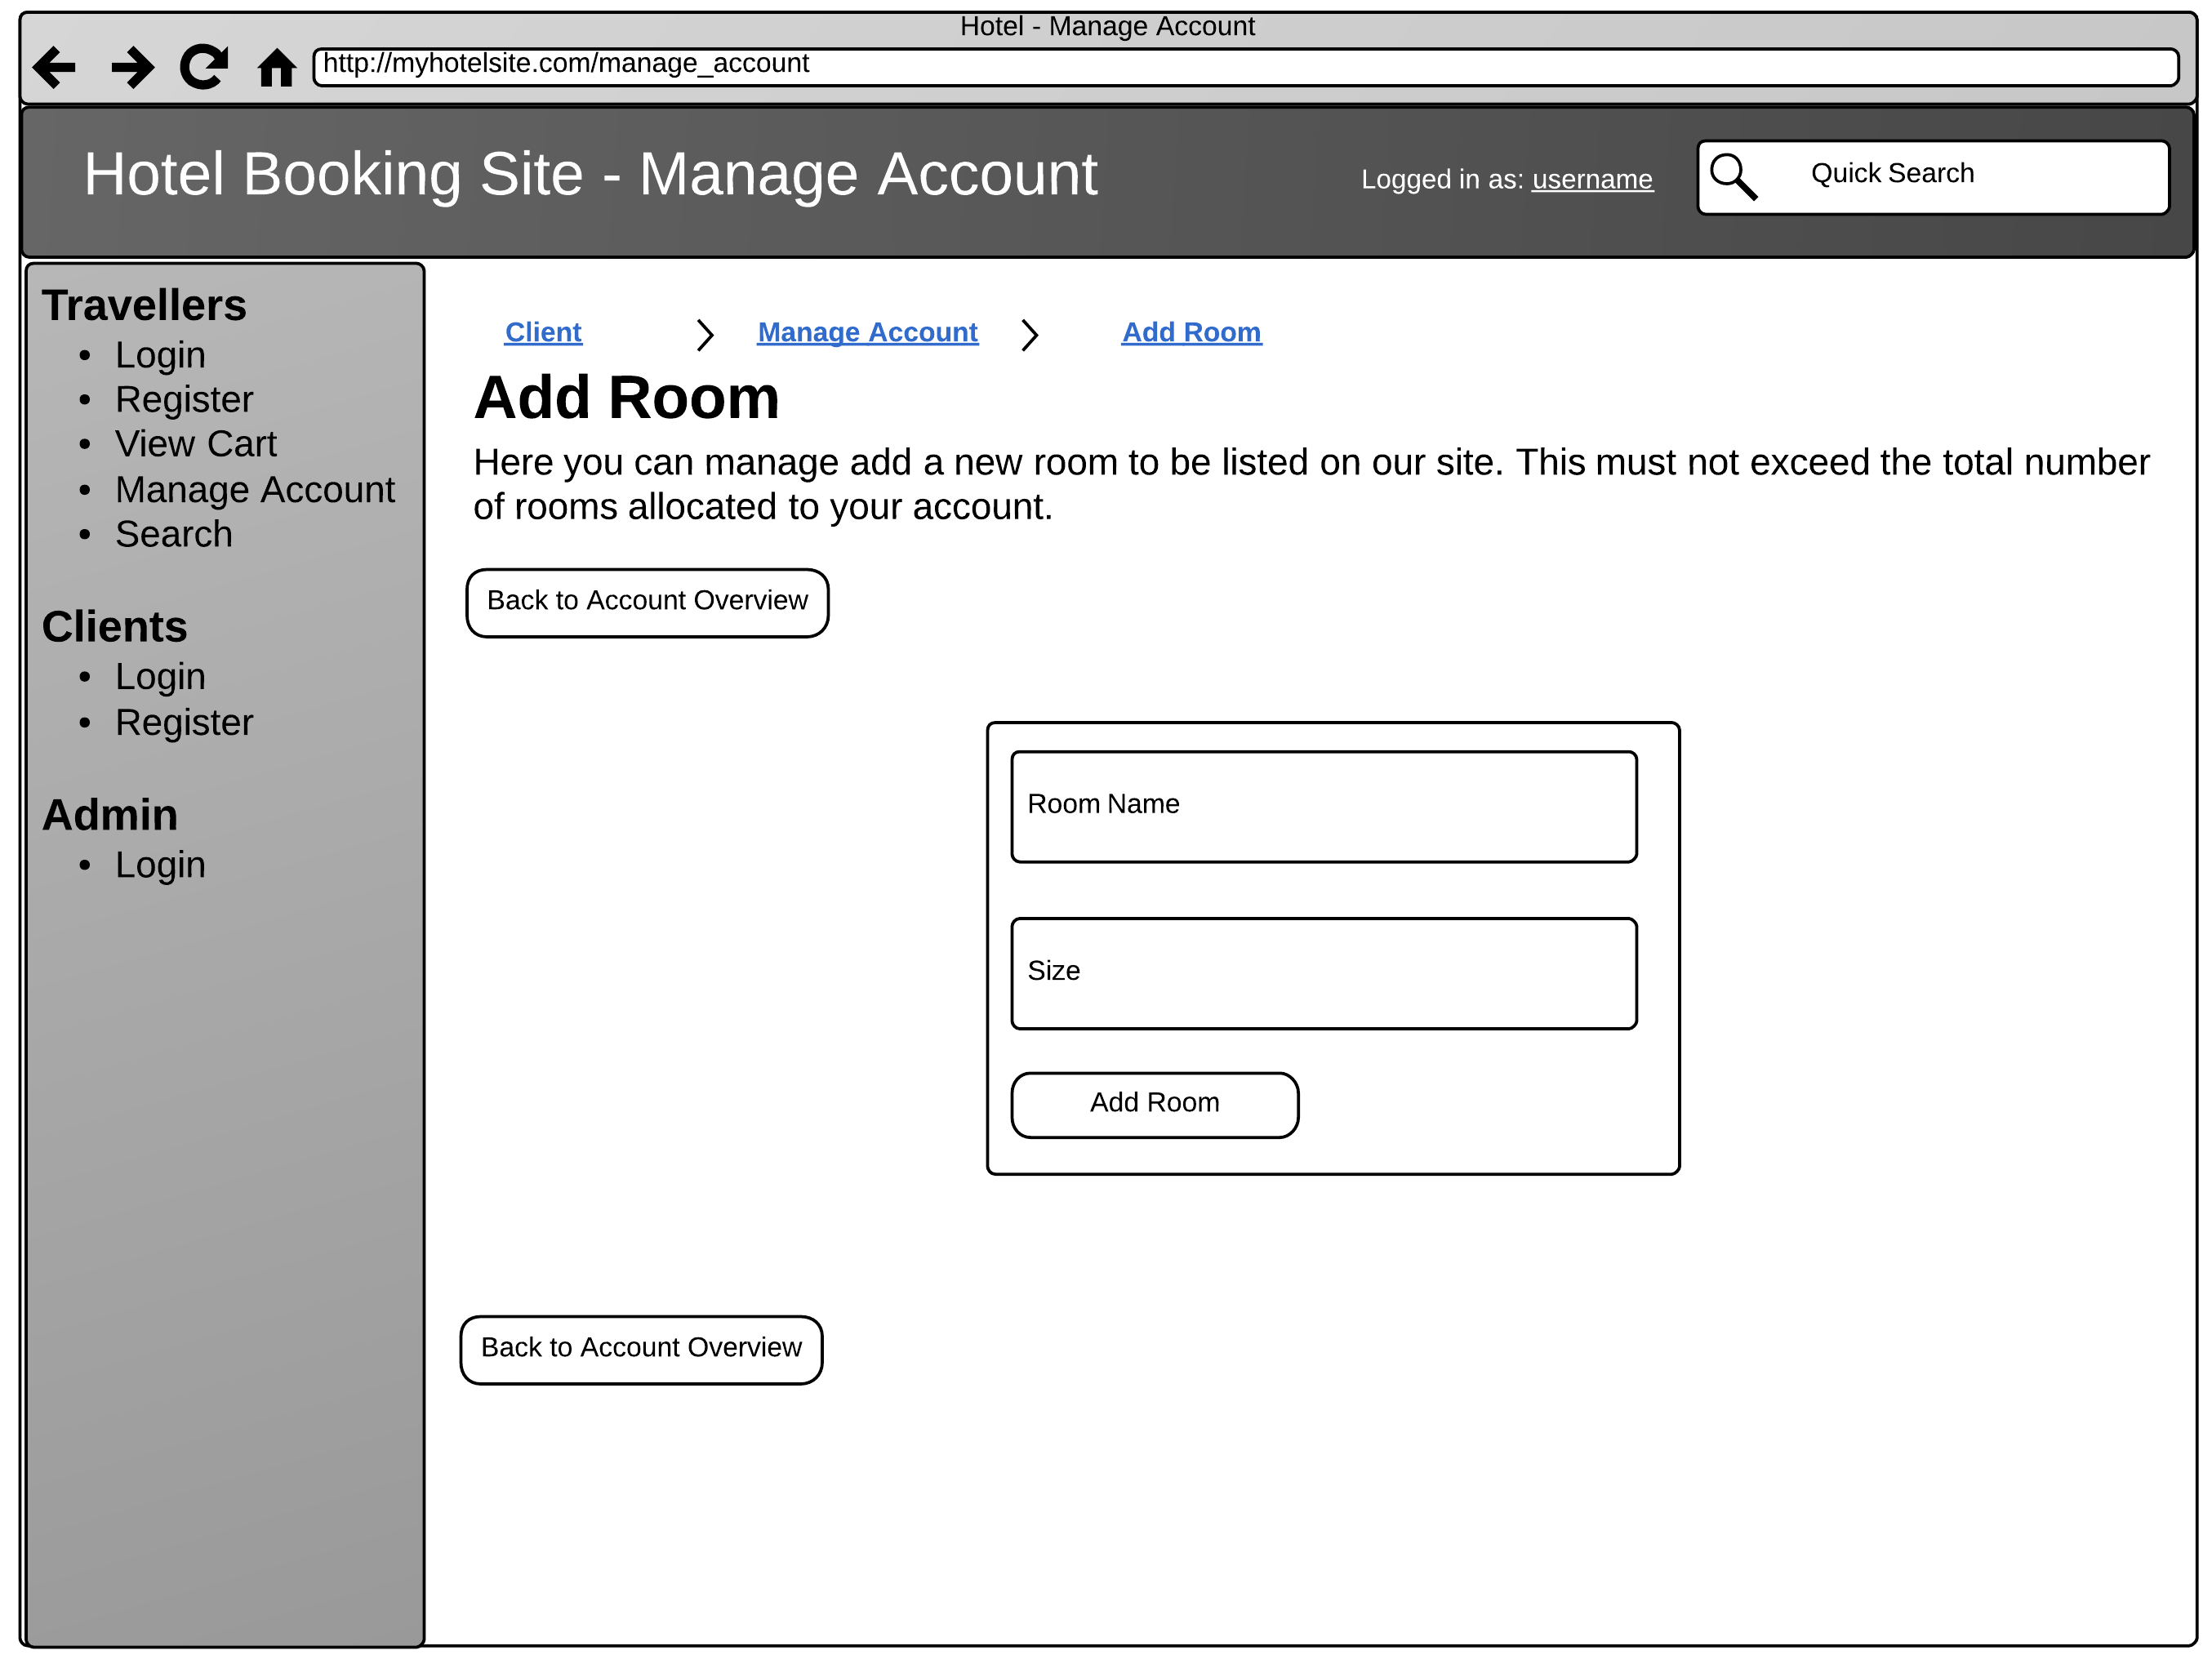
\includegraphics[width=0.7\textwidth]{img/wireframes/AddRoom.png}
\caption{Wireframe for adding a new room to the system.}
\label{fig:wireframe-client-add-room}
\end{figure}

\begin{figure}[H]
\centering
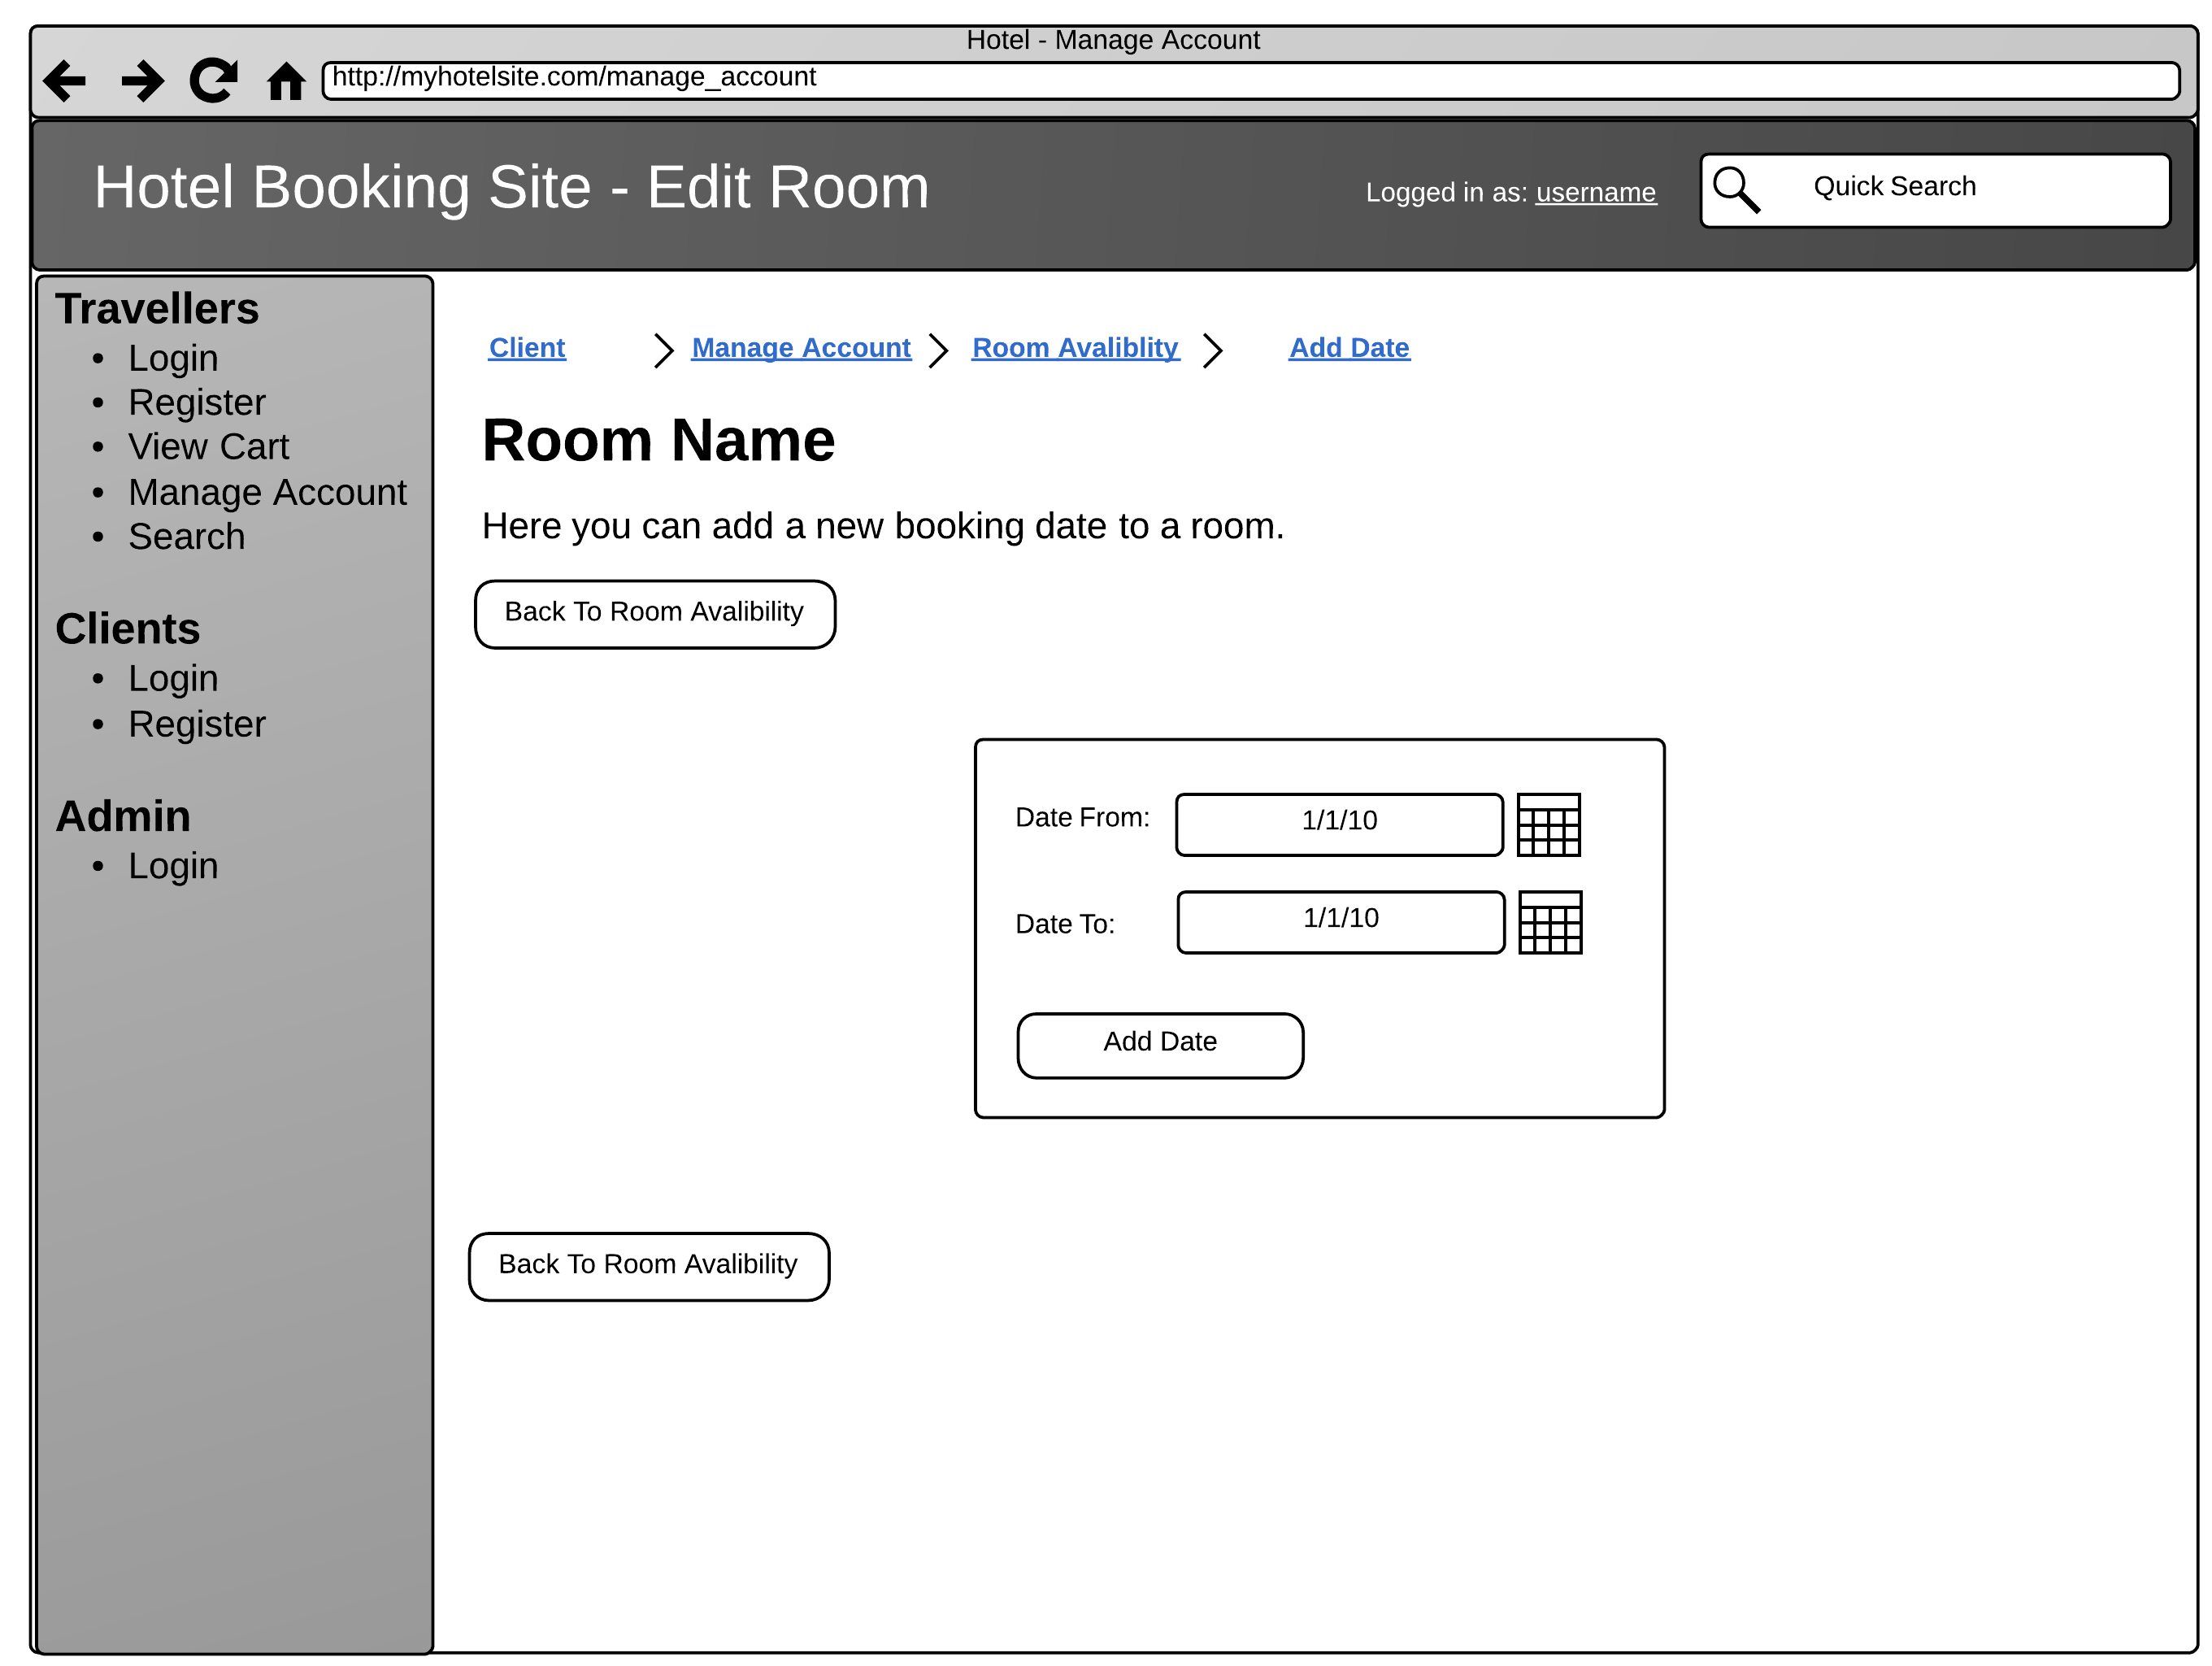
\includegraphics[width=0.7\textwidth]{img/wireframes/AddDate.png}
\caption{Wireframe for adding a new booking date to the system.}
\label{fig:wireframe-client-add-date}
\end{figure}

\subsection{Administrator Account Management}
For the management page of the administrator account I have simply listed the details of each hotel that is requesting authorisation for an account and provided clear options to either accept or decline the request. The details about the registration request will include whether the request is for an allocation model account or a referral model account.

\begin{figure}[H]
\centering
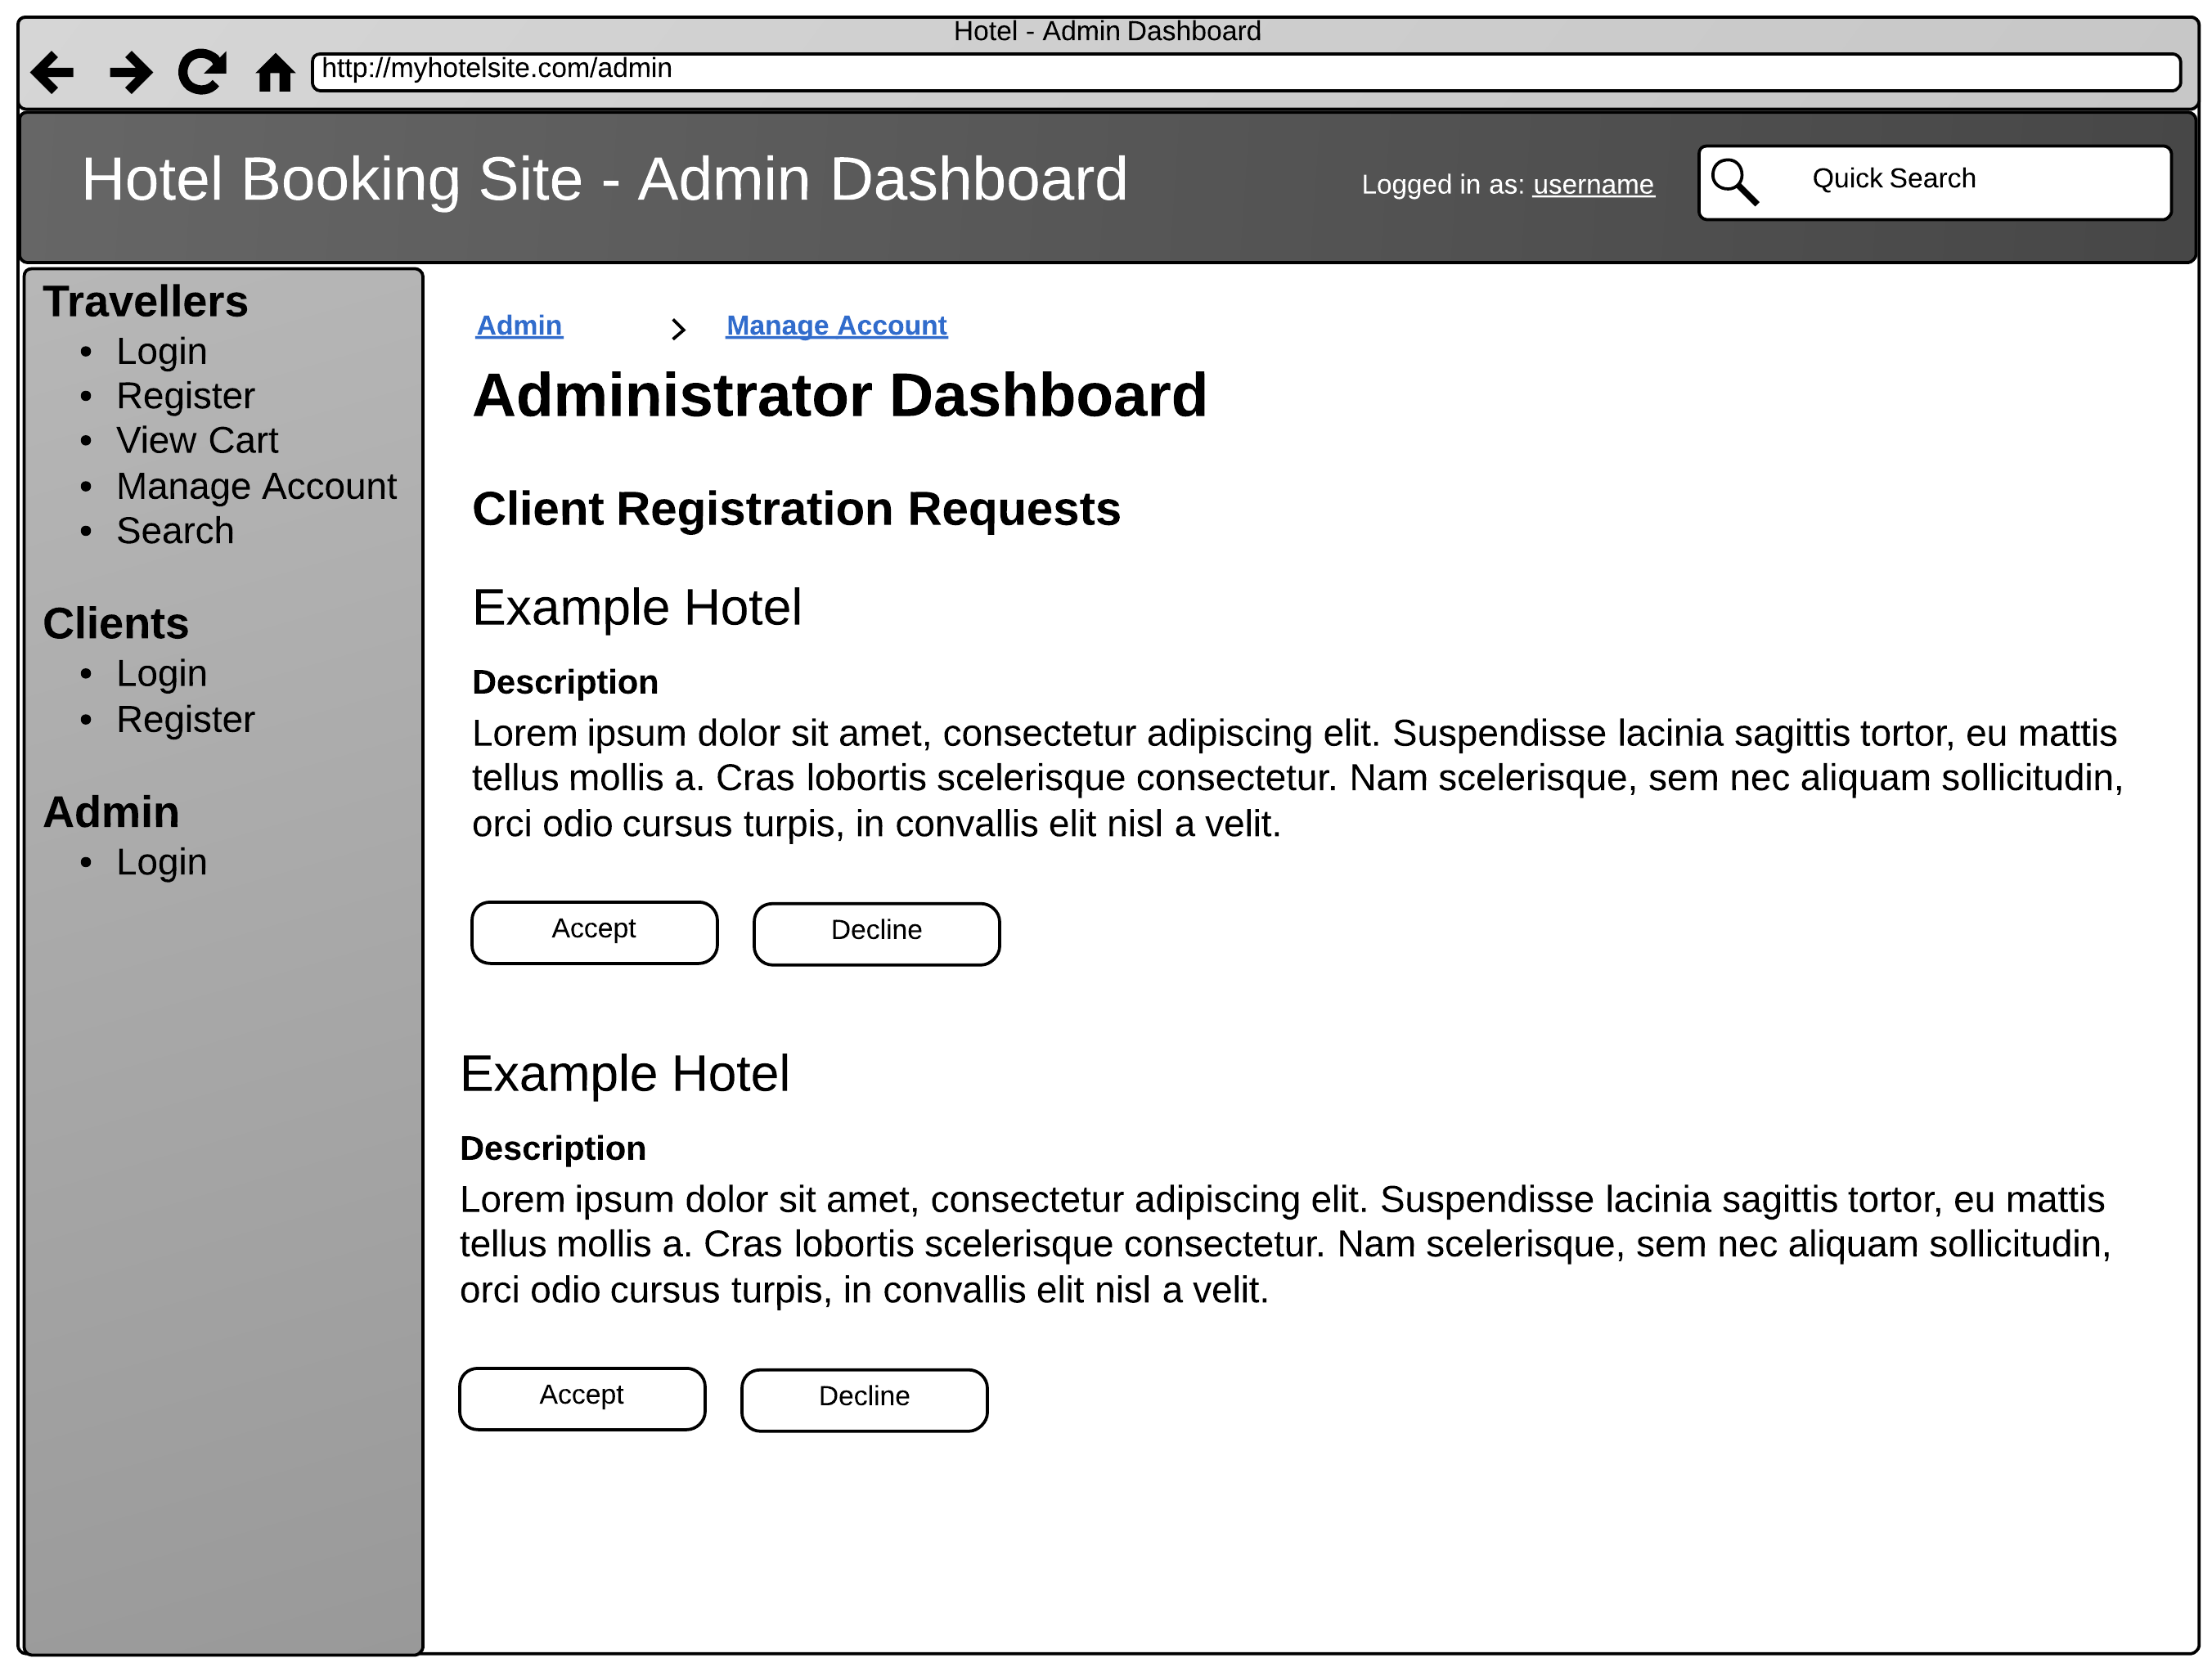
\includegraphics[width=0.7\textwidth]{img/wireframes/Administrator.png}
\caption{Wireframe for Admin management page.}
\label{fig:wireframe-client-register}
\end{figure}


\subsection{Traveller Search}
Traveller search is one of the major functions a user can perform on the site. This page simply provides a form for the user to search for accommodation on the site and filter it using the fields provided. As an example of what criteria might be used to filter search results, I've shown the form with field for searching by: Hotel name, Location, type (i.e. Guest House/Hotel) star rating and the dates the accommodation is available from and until.

\begin{figure}[H]
\centering
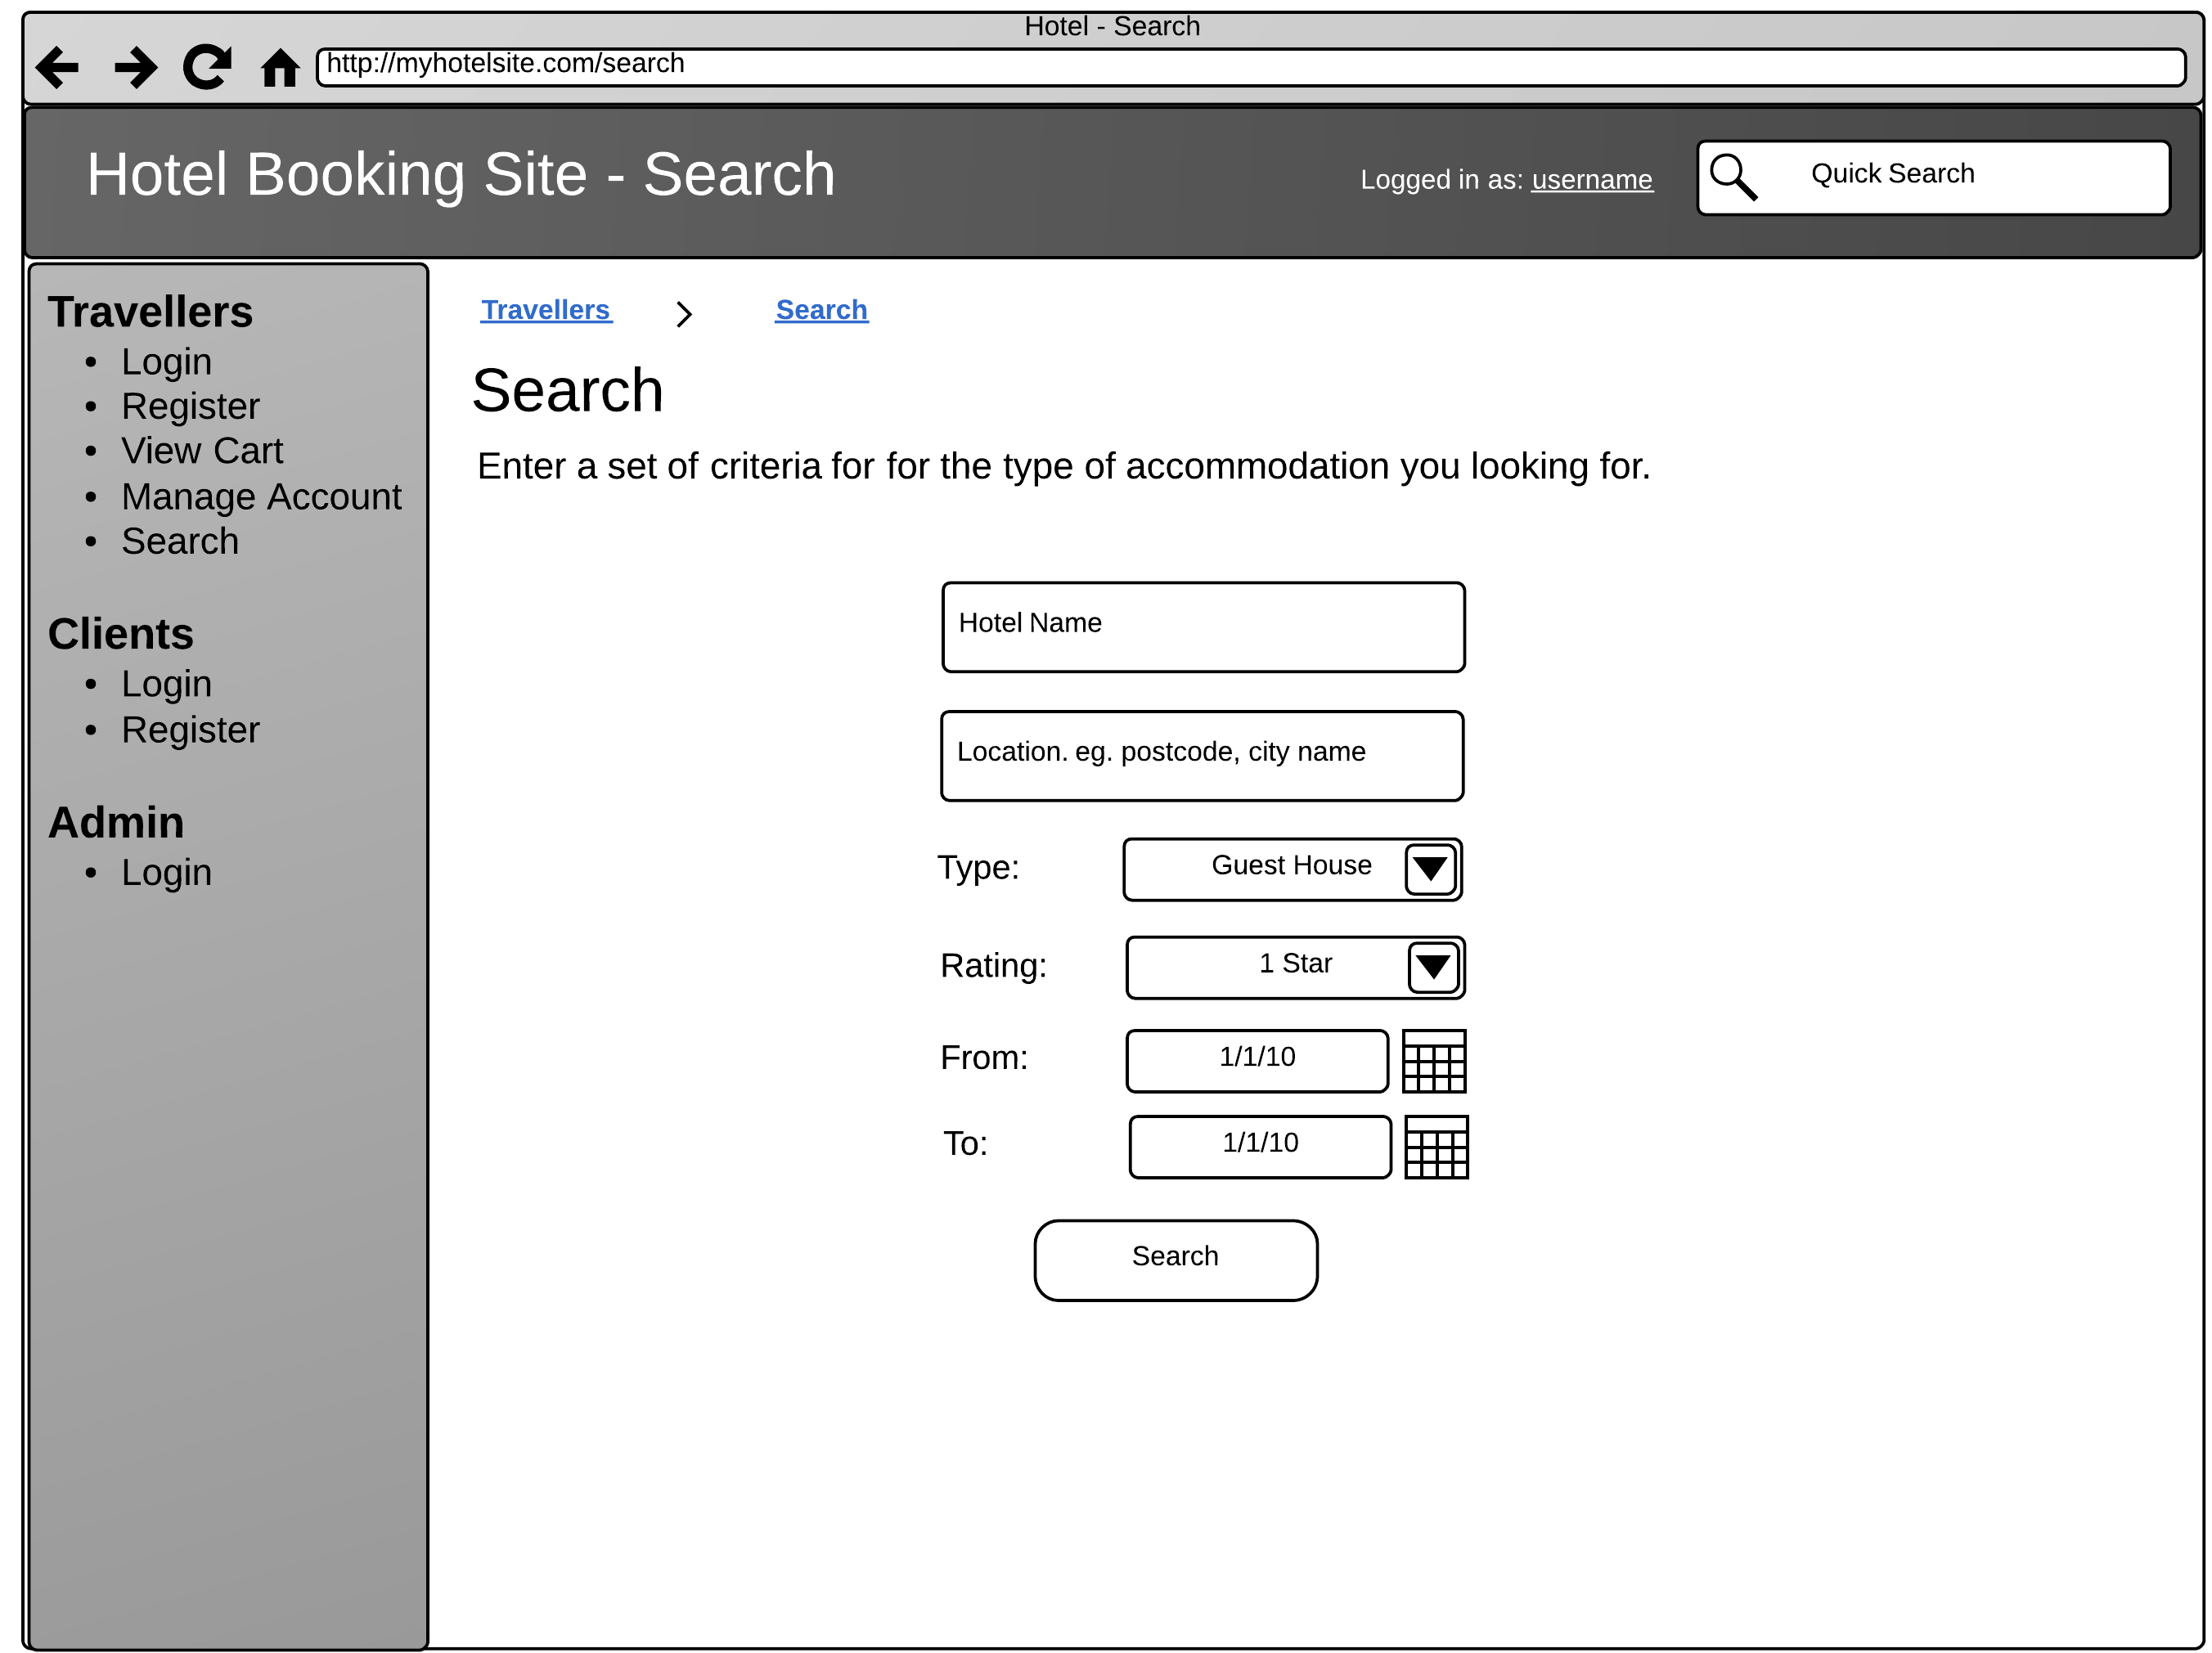
\includegraphics[width=0.7\textwidth]{img/wireframes/Search.png}
\caption{Wireframe for Traveller search page.}
\label{fig:wireframe-traveller-search}
\end{figure}

Pressing search on the search page will take the user to the following wireframe design shown in figure \ref{fig:wireframe-traveller-results}. This shows the user a list of results that met their specified search criteria. Each result item will provide a description of the hotel, the cost of the accommodation and the ability to add the item to the user's cart. If the site was implemented fully, I would expect results to be added to the cart from this page either on the click of the add to cart button either by AJAX or by a page refresh. 

This page provides navigation buttons to go "forward" in the search/booking flow to view there cart or "backwards" to refine there search criteria. Like other pages, this page has a set of navigation controls at the top and bottom of the page to save the user having to scroll back to the top of the page.

\begin{figure}[H]
\centering
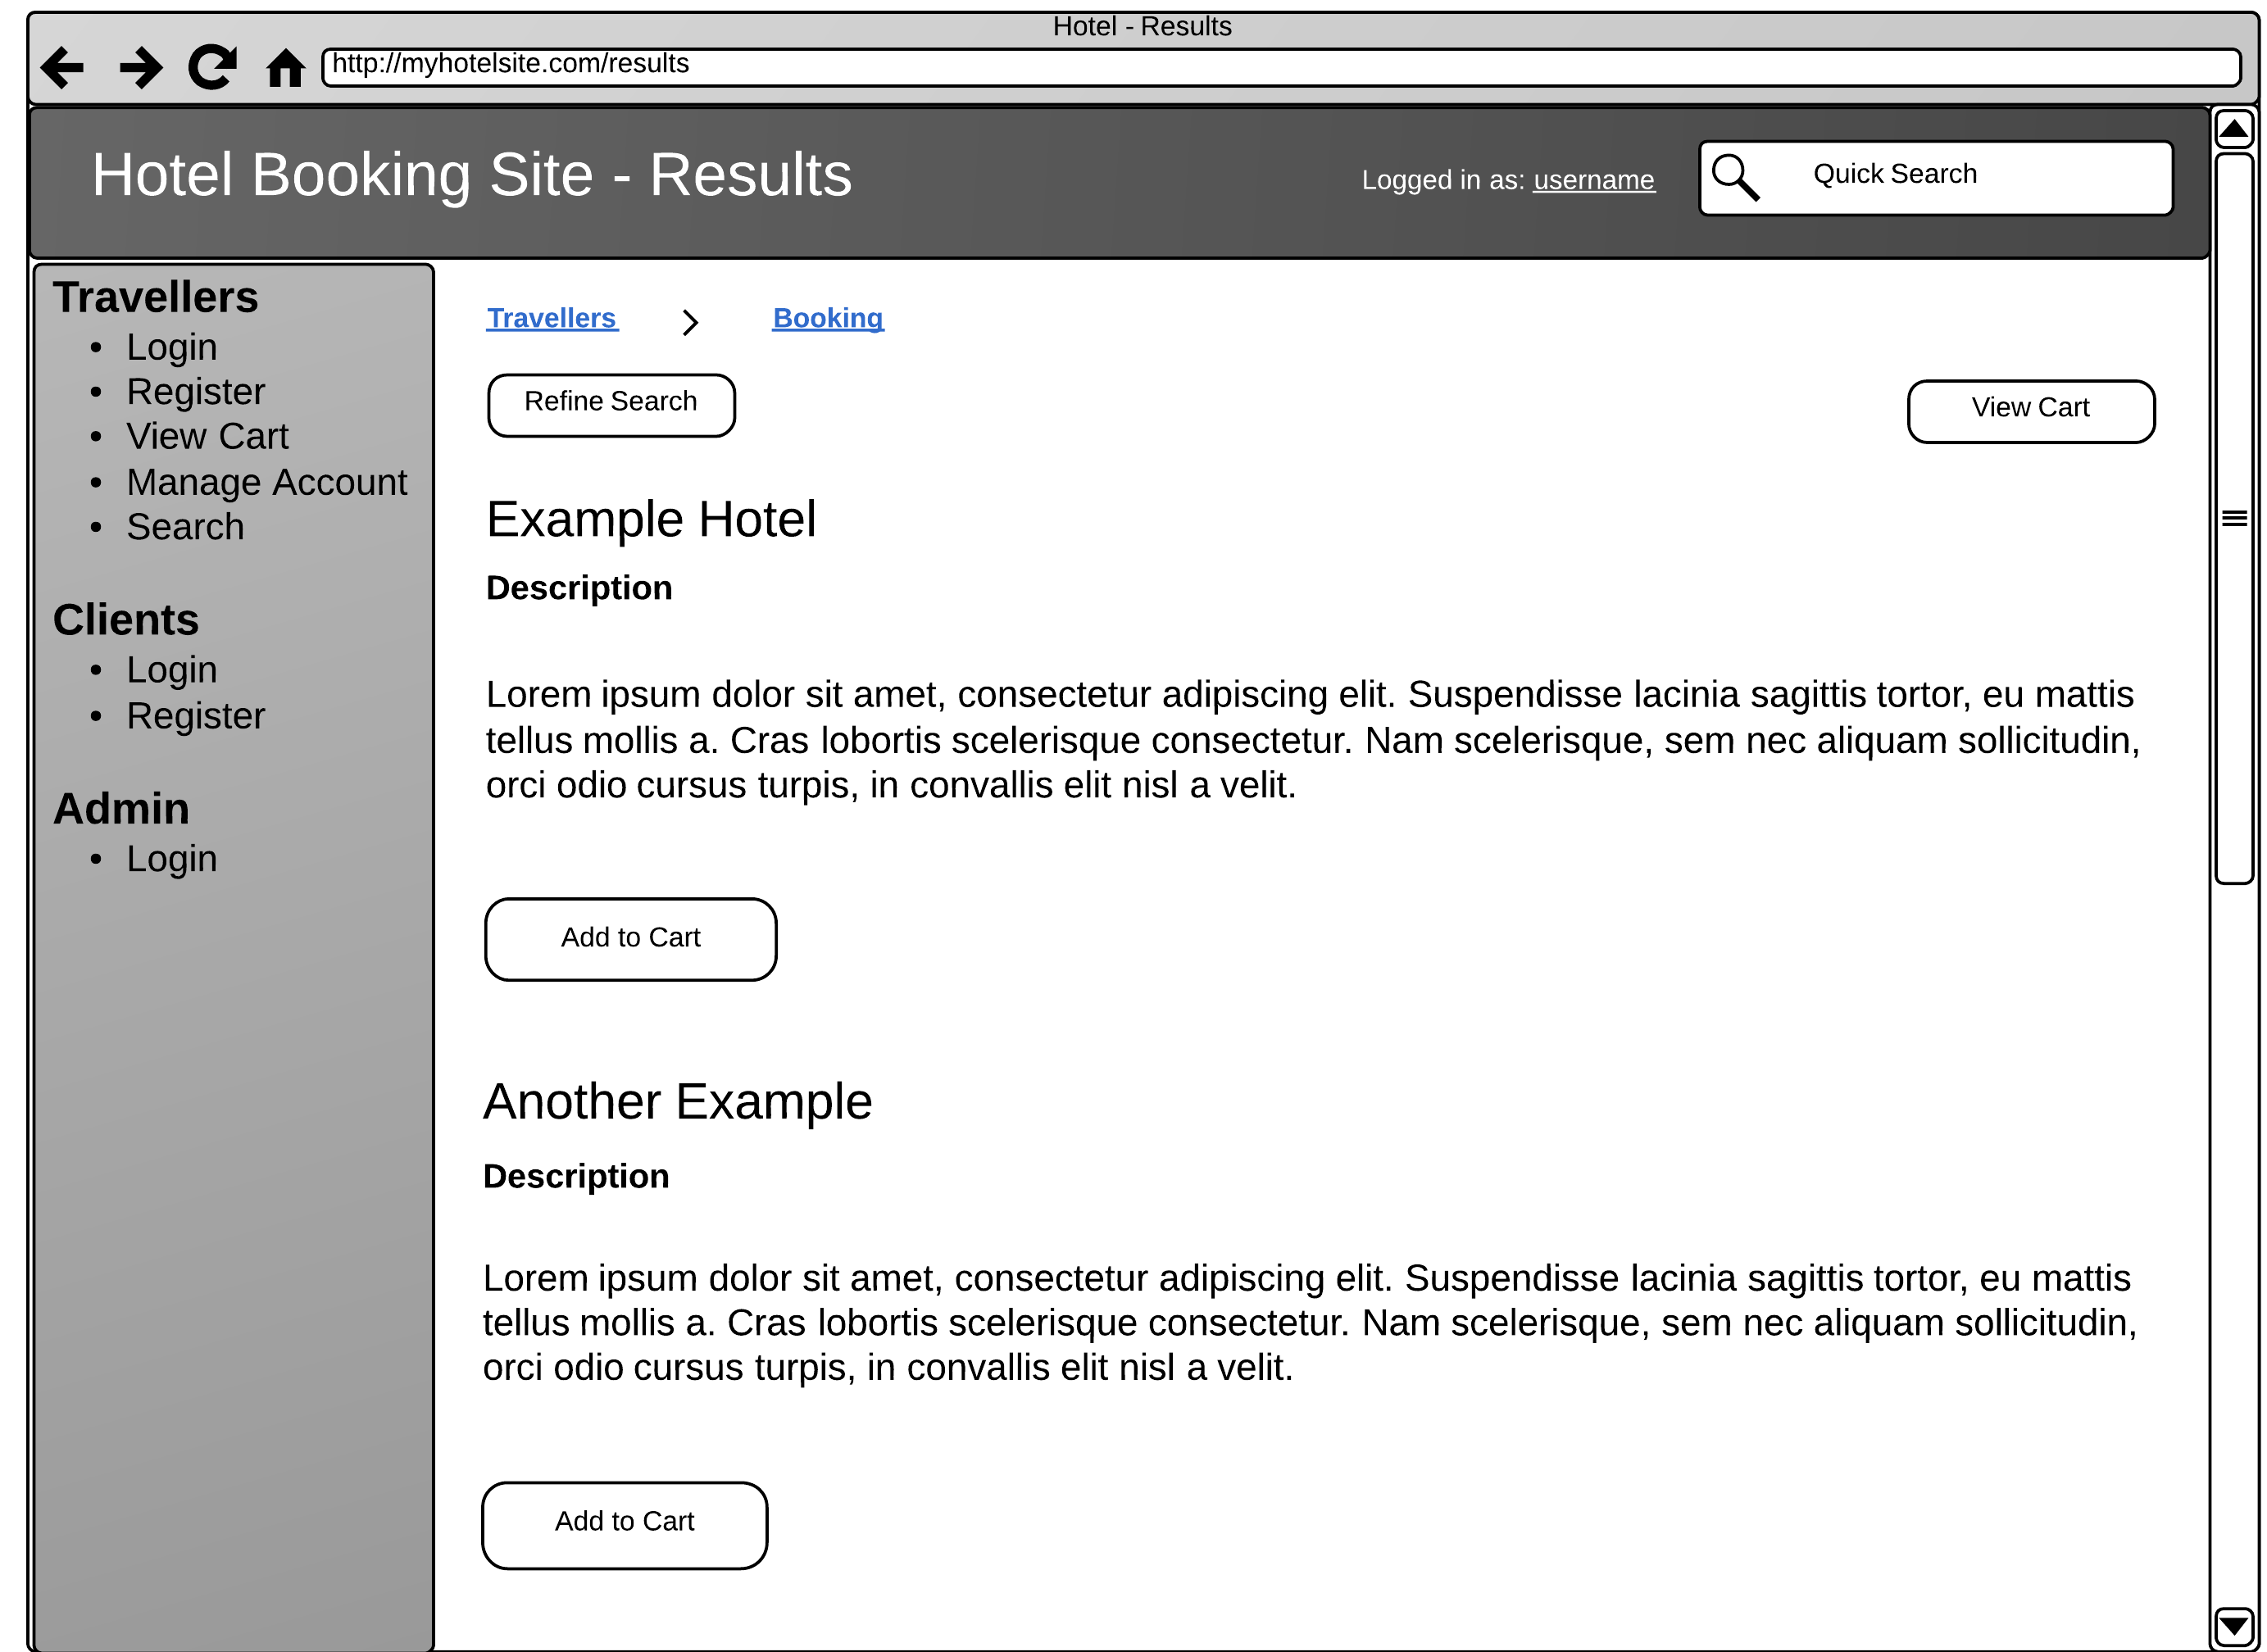
\includegraphics[width=0.7\textwidth]{img/wireframes/Results.png}
\caption{Wireframe for the results of a Traveller search.}
\label{fig:wireframe-traveller-results}
\end{figure}

\subsection{Traveller Booking}
The final section of the site, and probably the most important is the section which deals with taking the booking from customers. Firstly, after adding items to their cart from the search results, users can go navigate to their cart either thorough the side menu or via the navigational controls on the results page. This page will display all of the items they have selected to pay for and book. 

\begin{figure}[H]
\centering
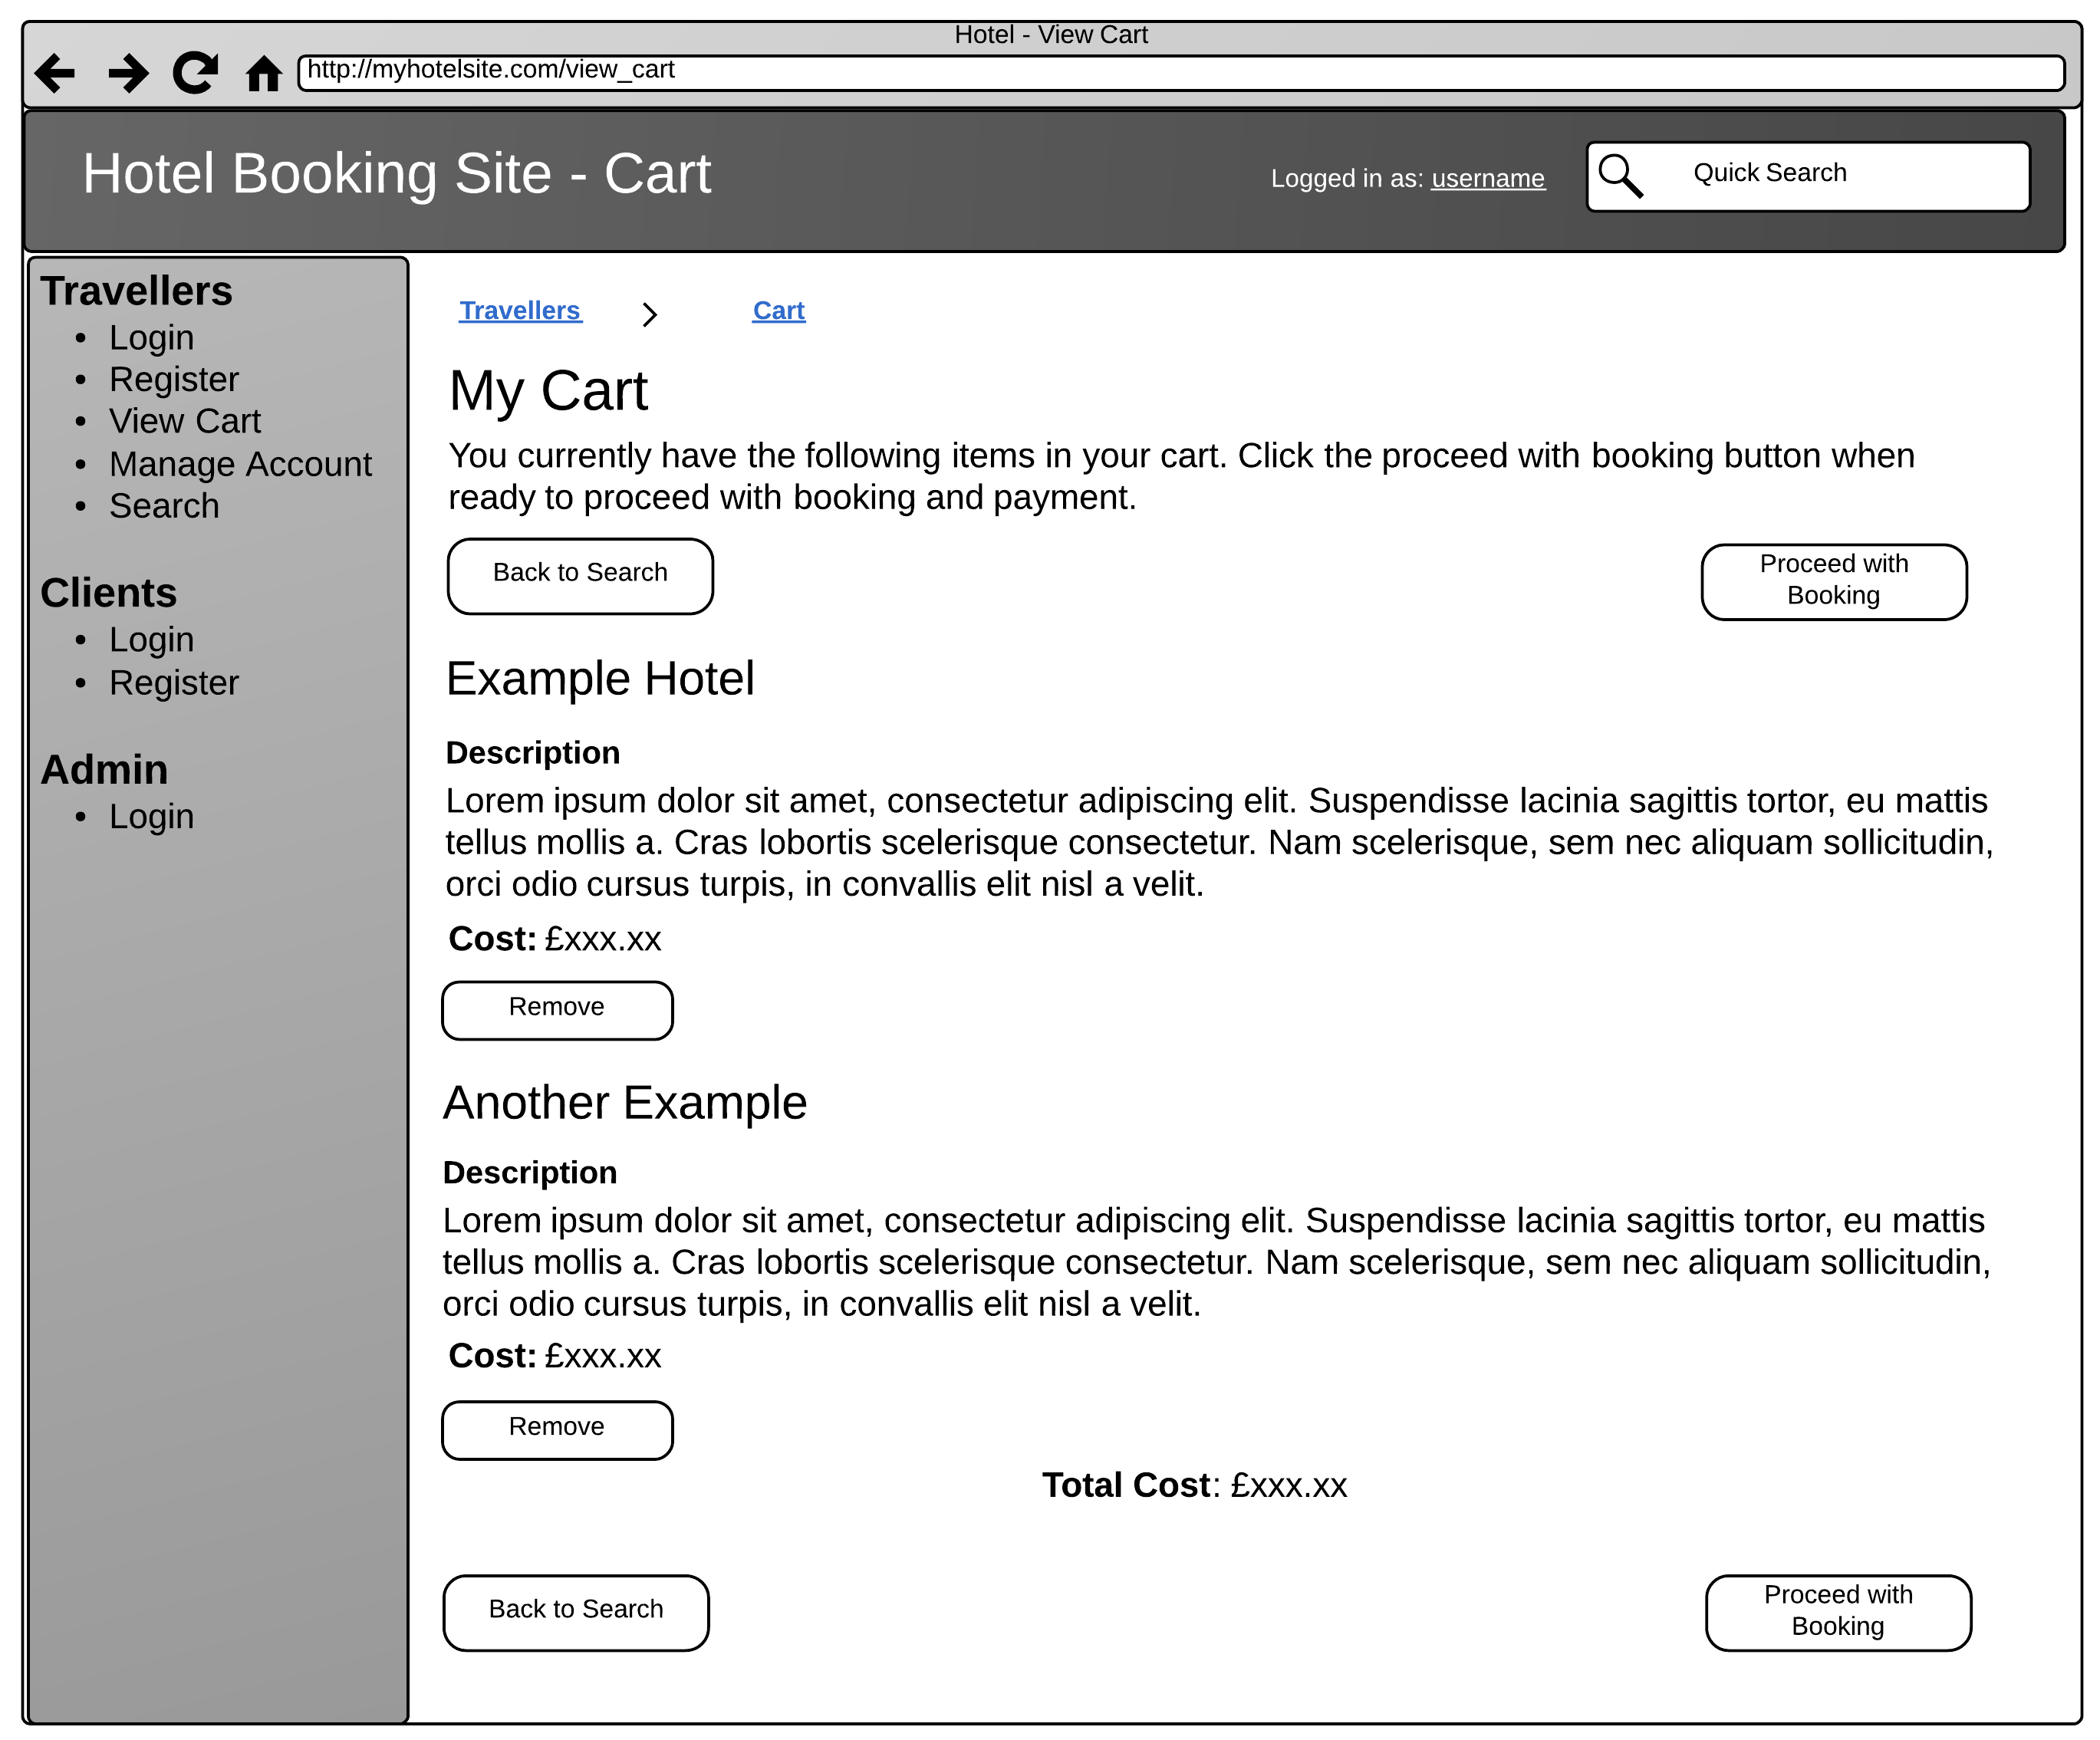
\includegraphics[width=0.7\textwidth]{img/wireframes/Cart.png}
\caption{Wireframe for the Traveller's cart.}
\label{fig:wireframe-traveller-cart}
\end{figure}

Again this page has a very similar design to previous pages for consistency. I have also include a note of the total cost of the basket at the top and bottom of the page, so that the Traveller can clearly see the overall cost of what they are paying for. The individual cost of each item is also displayed alongside each item description. Individual items can also be removed from the cart using the provided button.

\begin{figure}[H]
\centering
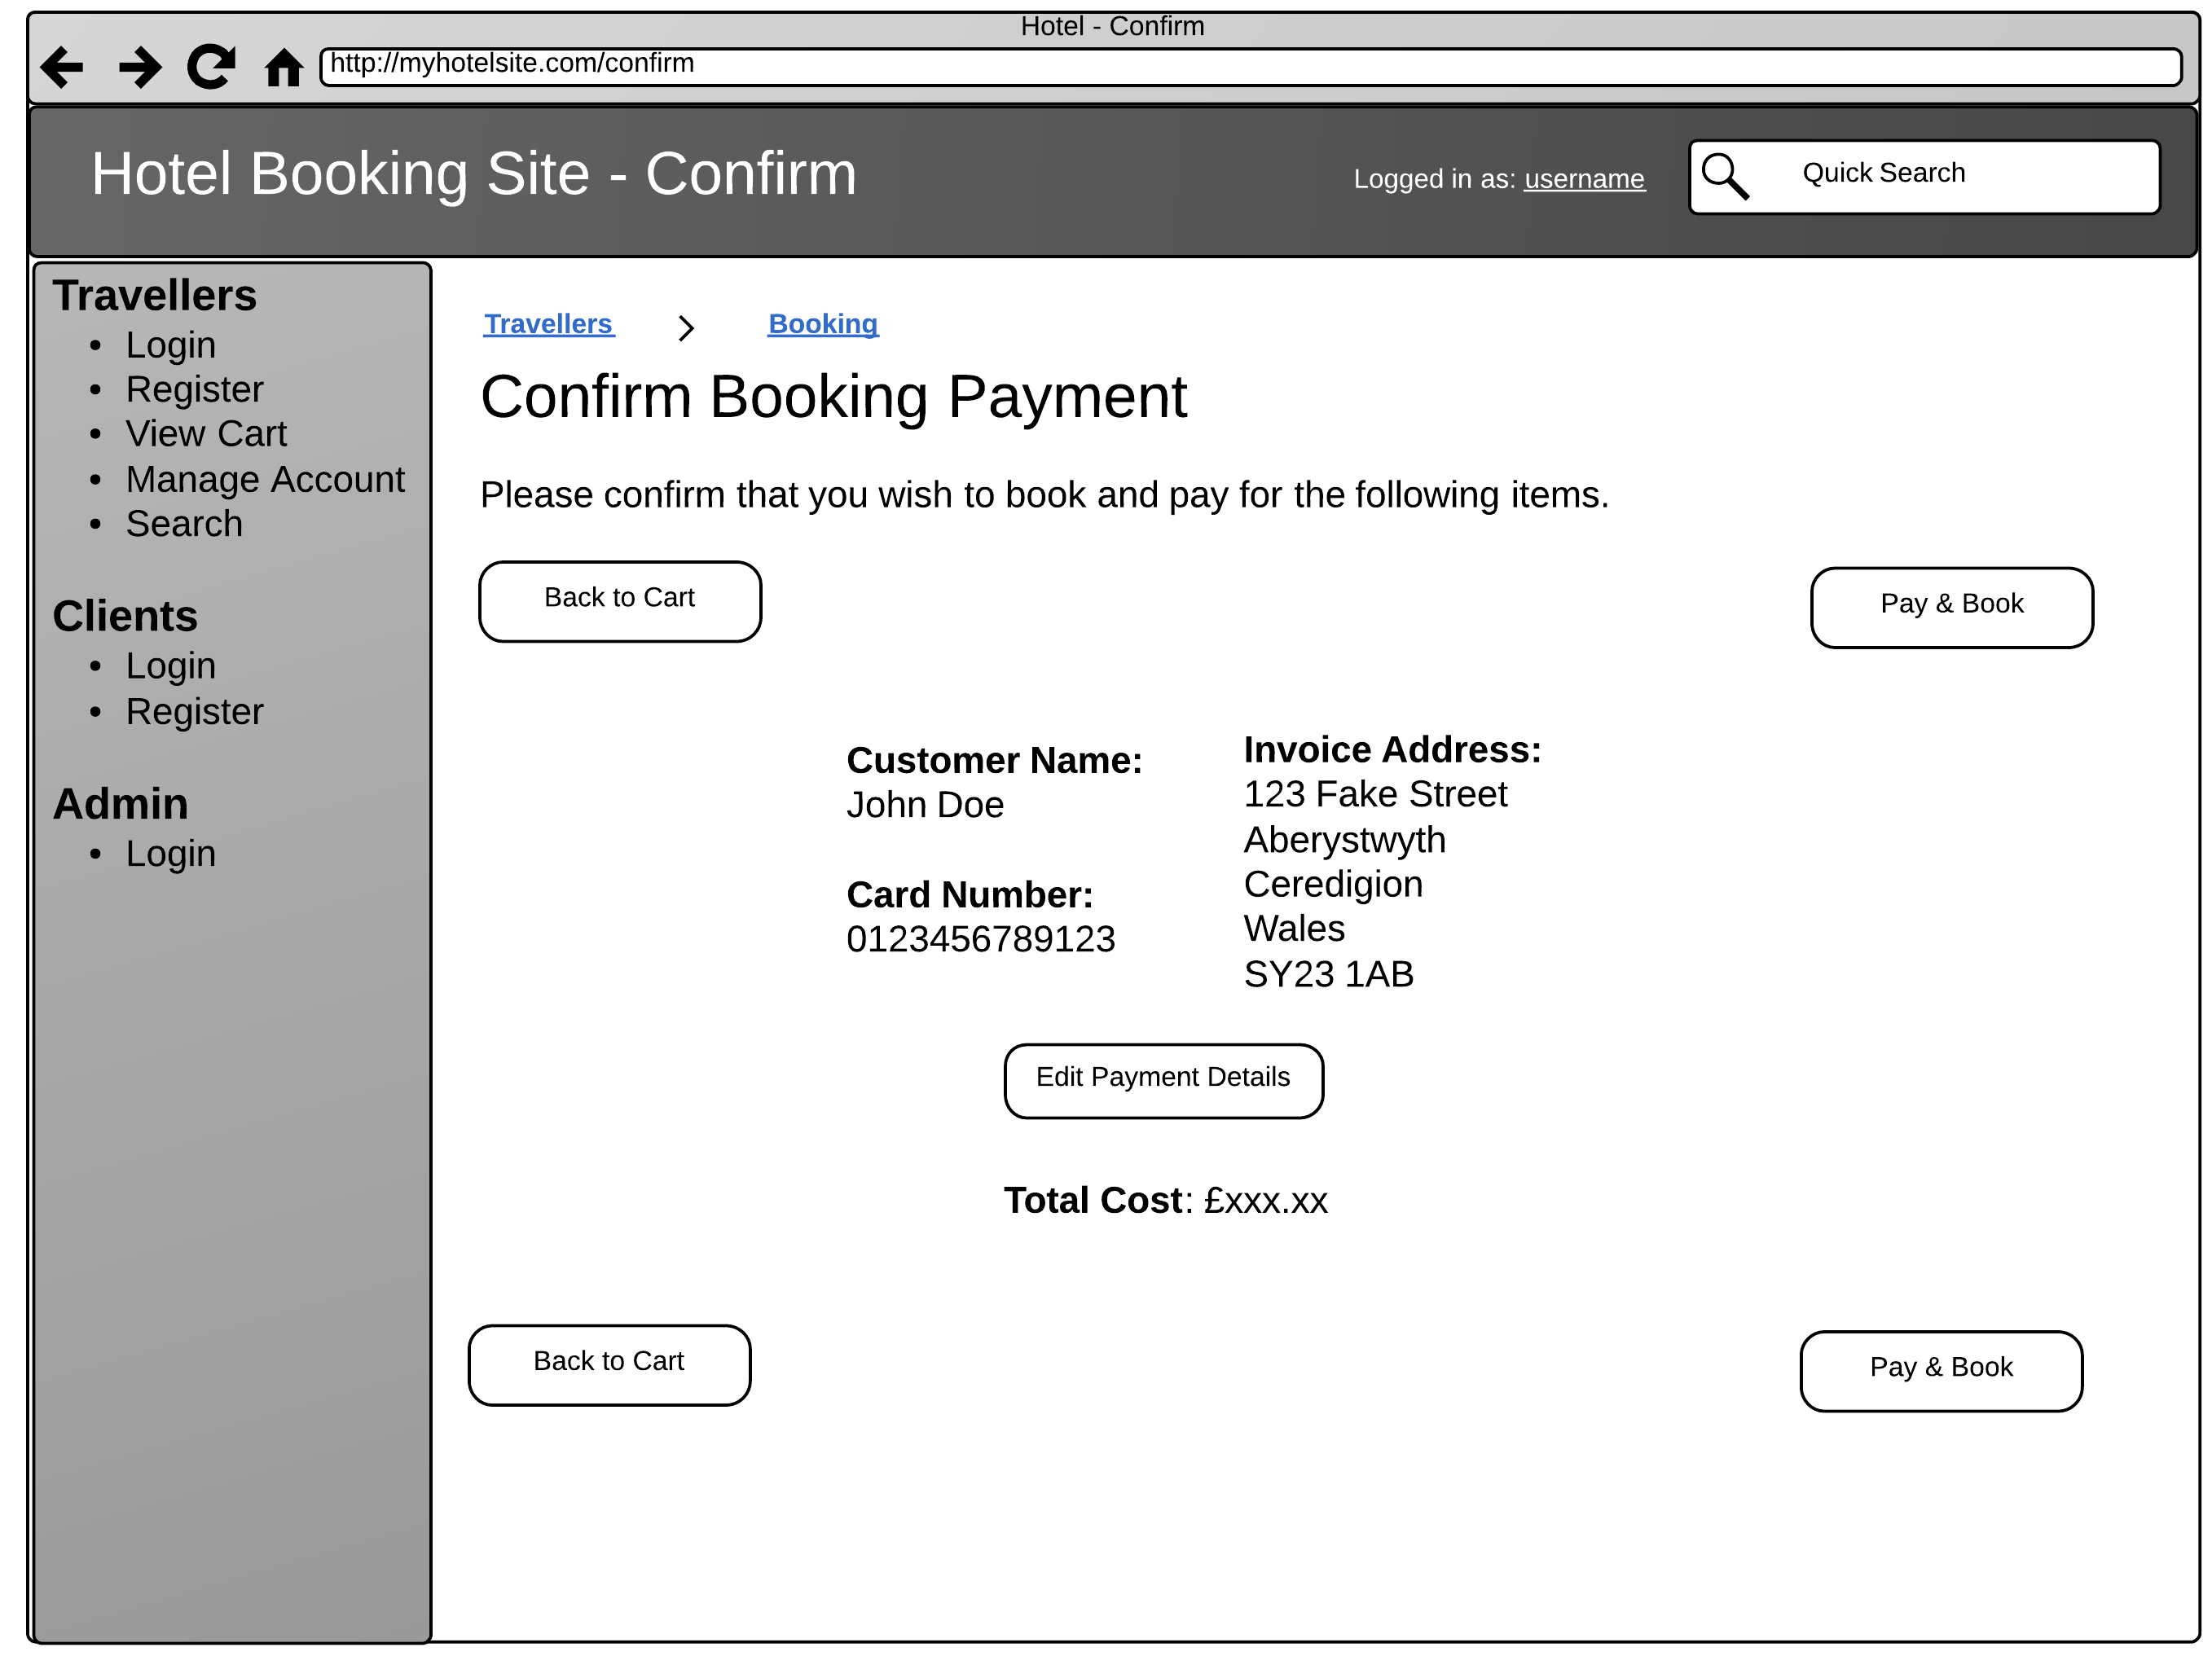
\includegraphics[width=0.7\textwidth]{img/wireframes/ConfirmBooking.png}
\caption{Wireframe for the page to confirm transaction details.}
\label{fig:wireframe-traveller-confirm}
\end{figure}

Once a Traveller has reviewed the contents of their cart they can use the proceed with booking button to once again move forward with their transaction. At this point, if the user isn't already logged in they will be prompted to do so. If they do not have an account then they can make one. 

Once they are authenticated onto the system they will then be directed to the page shown in figure \ref{fig:wireframe-traveller-confirm} where they can review their payment details before making the transaction. The total cost is again provided along with the name, card number and billing address. A button is also available for the user to easily edit their details should they wish.

The final two wireframes, figures \ref{fig:wireframe-traveller-booked} and \ref{fig:wireframe-traveller-pending}, show what happens when the user presses the pay and book button the previous page depending on the hotel's model type. If they are using the allocation model, the booking is made and the Traveller is shown the booking confirmation page. Otherwise, if the hotel is using the referral model, the user is shown the pending page so they know that there transaction is complete but pending review from the hotel.

\begin{figure}[H]
\centering
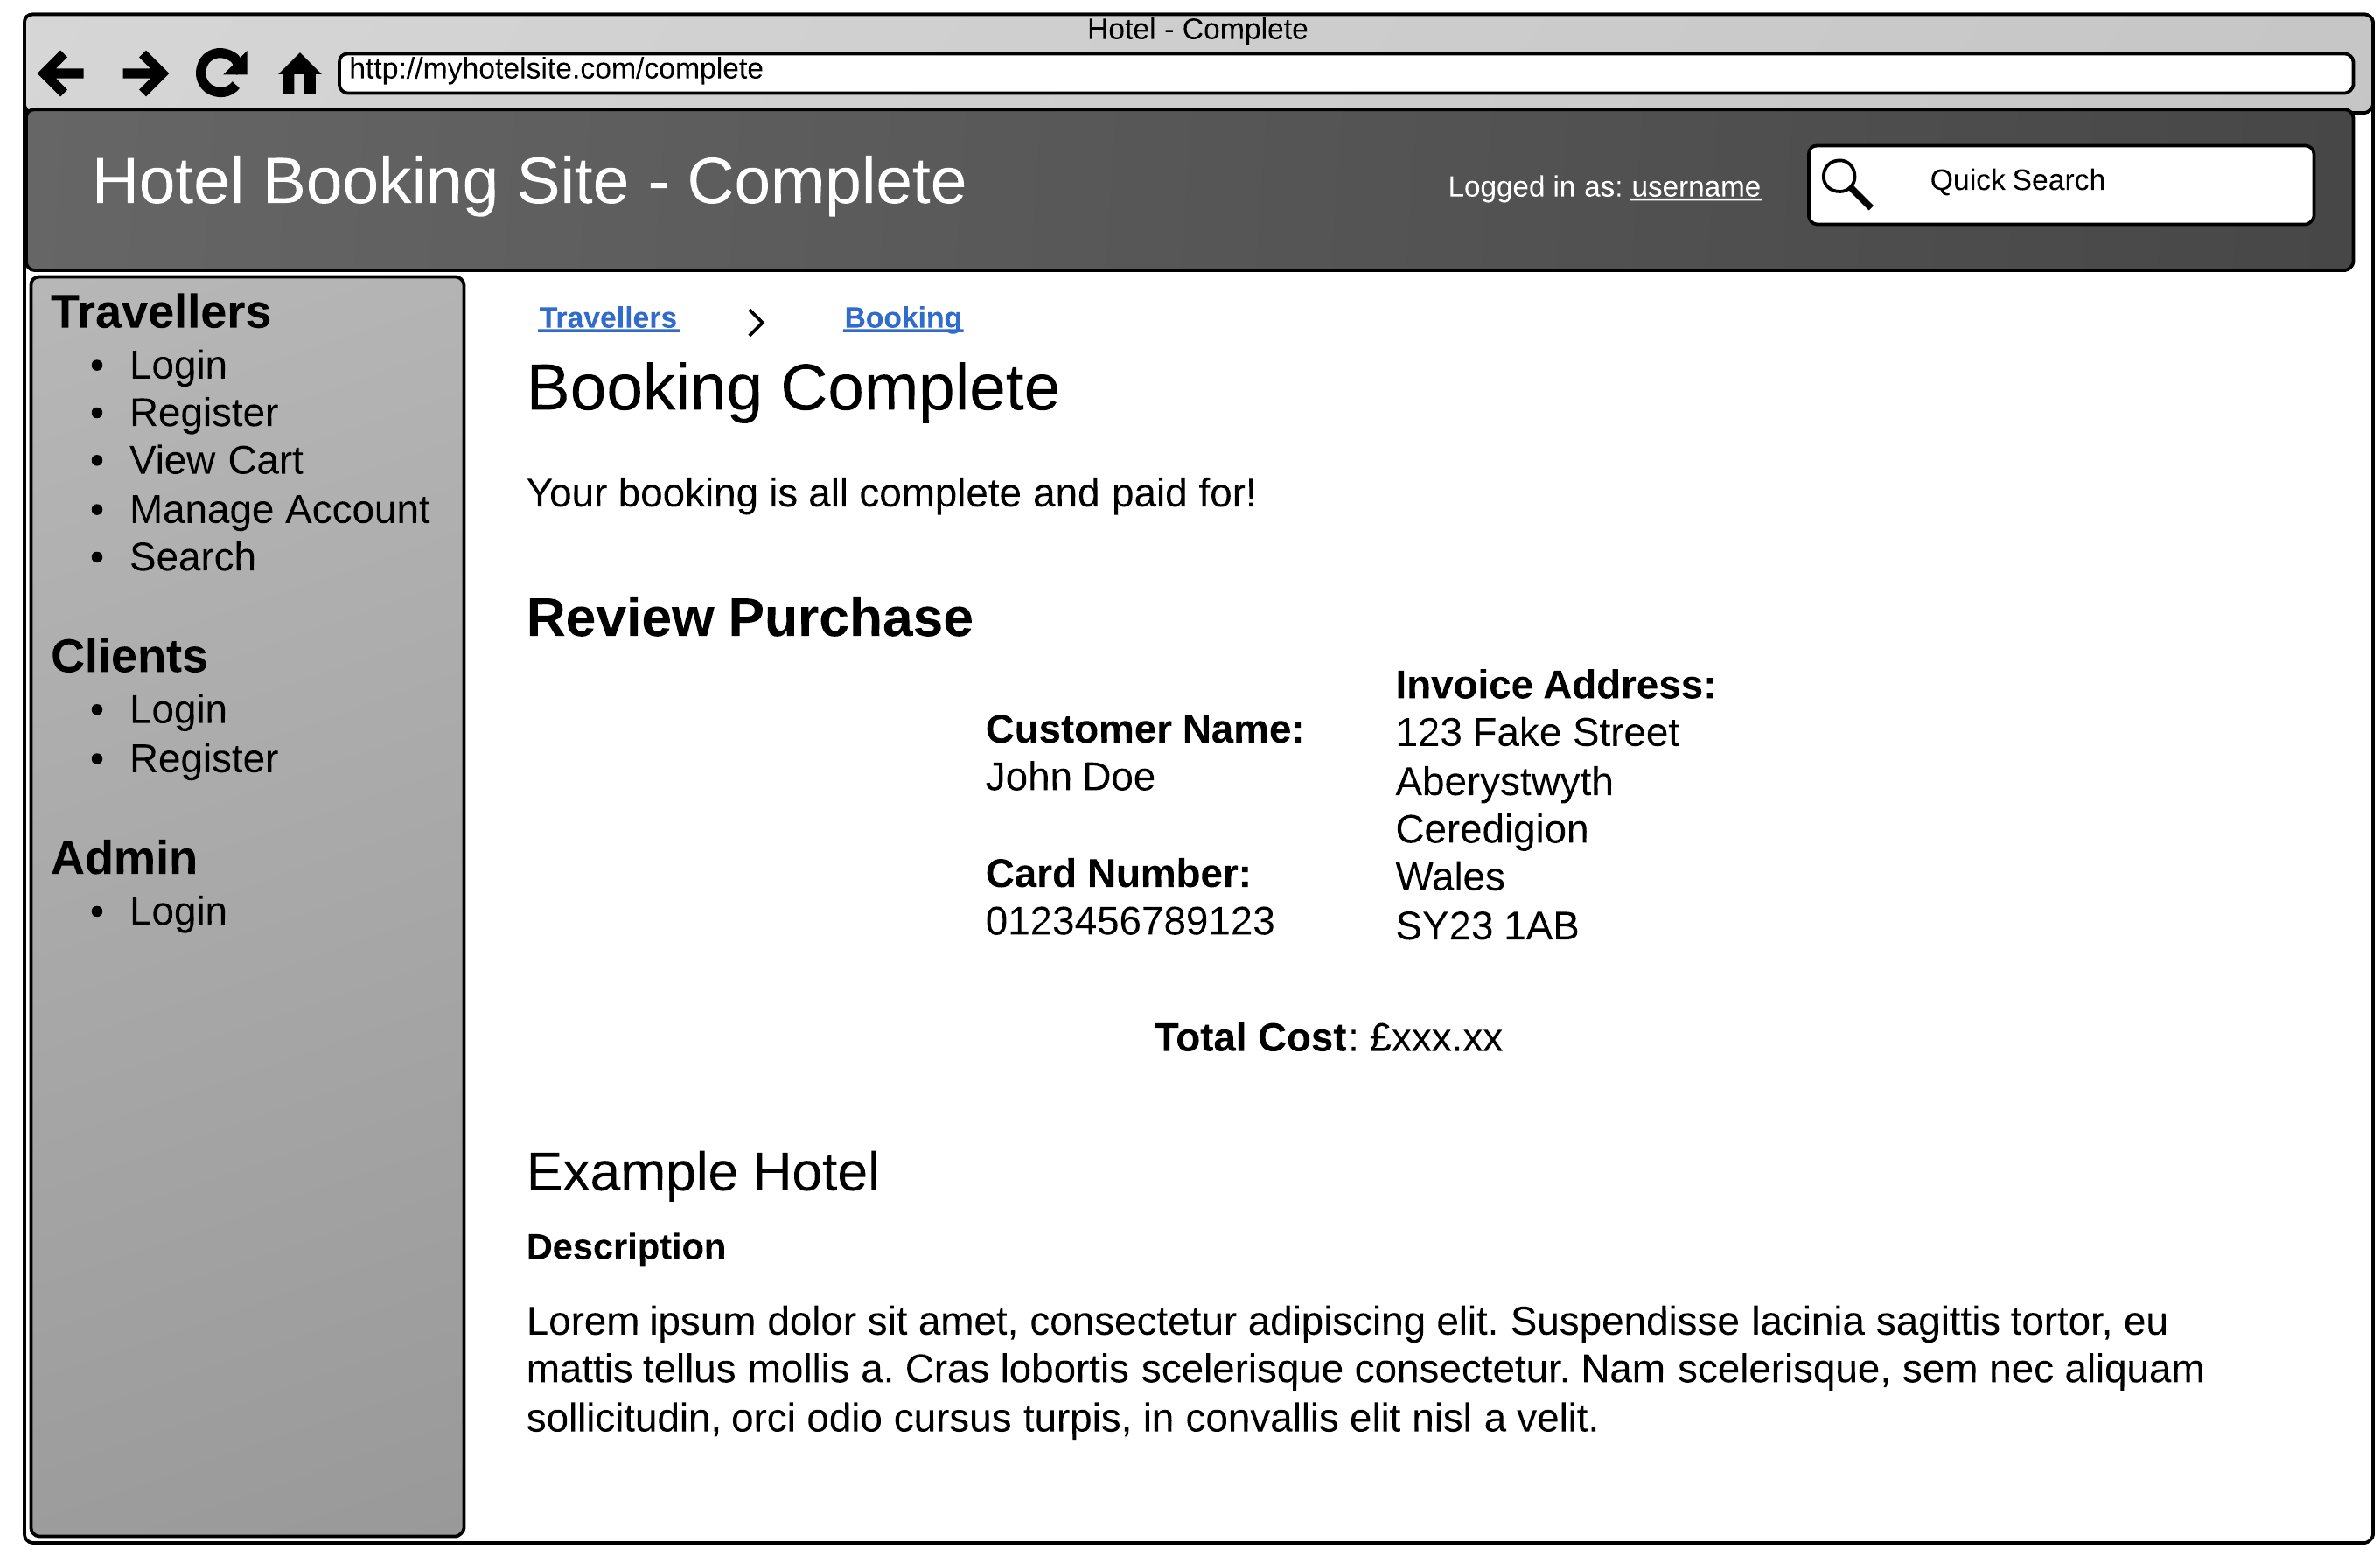
\includegraphics[width=0.7\textwidth]{img/wireframes/Booked.png}
\caption{Wireframe for the page shown on a confirmed booking.}
\label{fig:wireframe-traveller-booked}
\end{figure}

Both of these pages provide a clear review of what the customer has paid for and the details they use to make the purchase. These two page as designed to be definitive endpoint for the transaction process and therefore do not have any navigational elements available for the customer to "go back a step".

\begin{figure}[H]
\centering
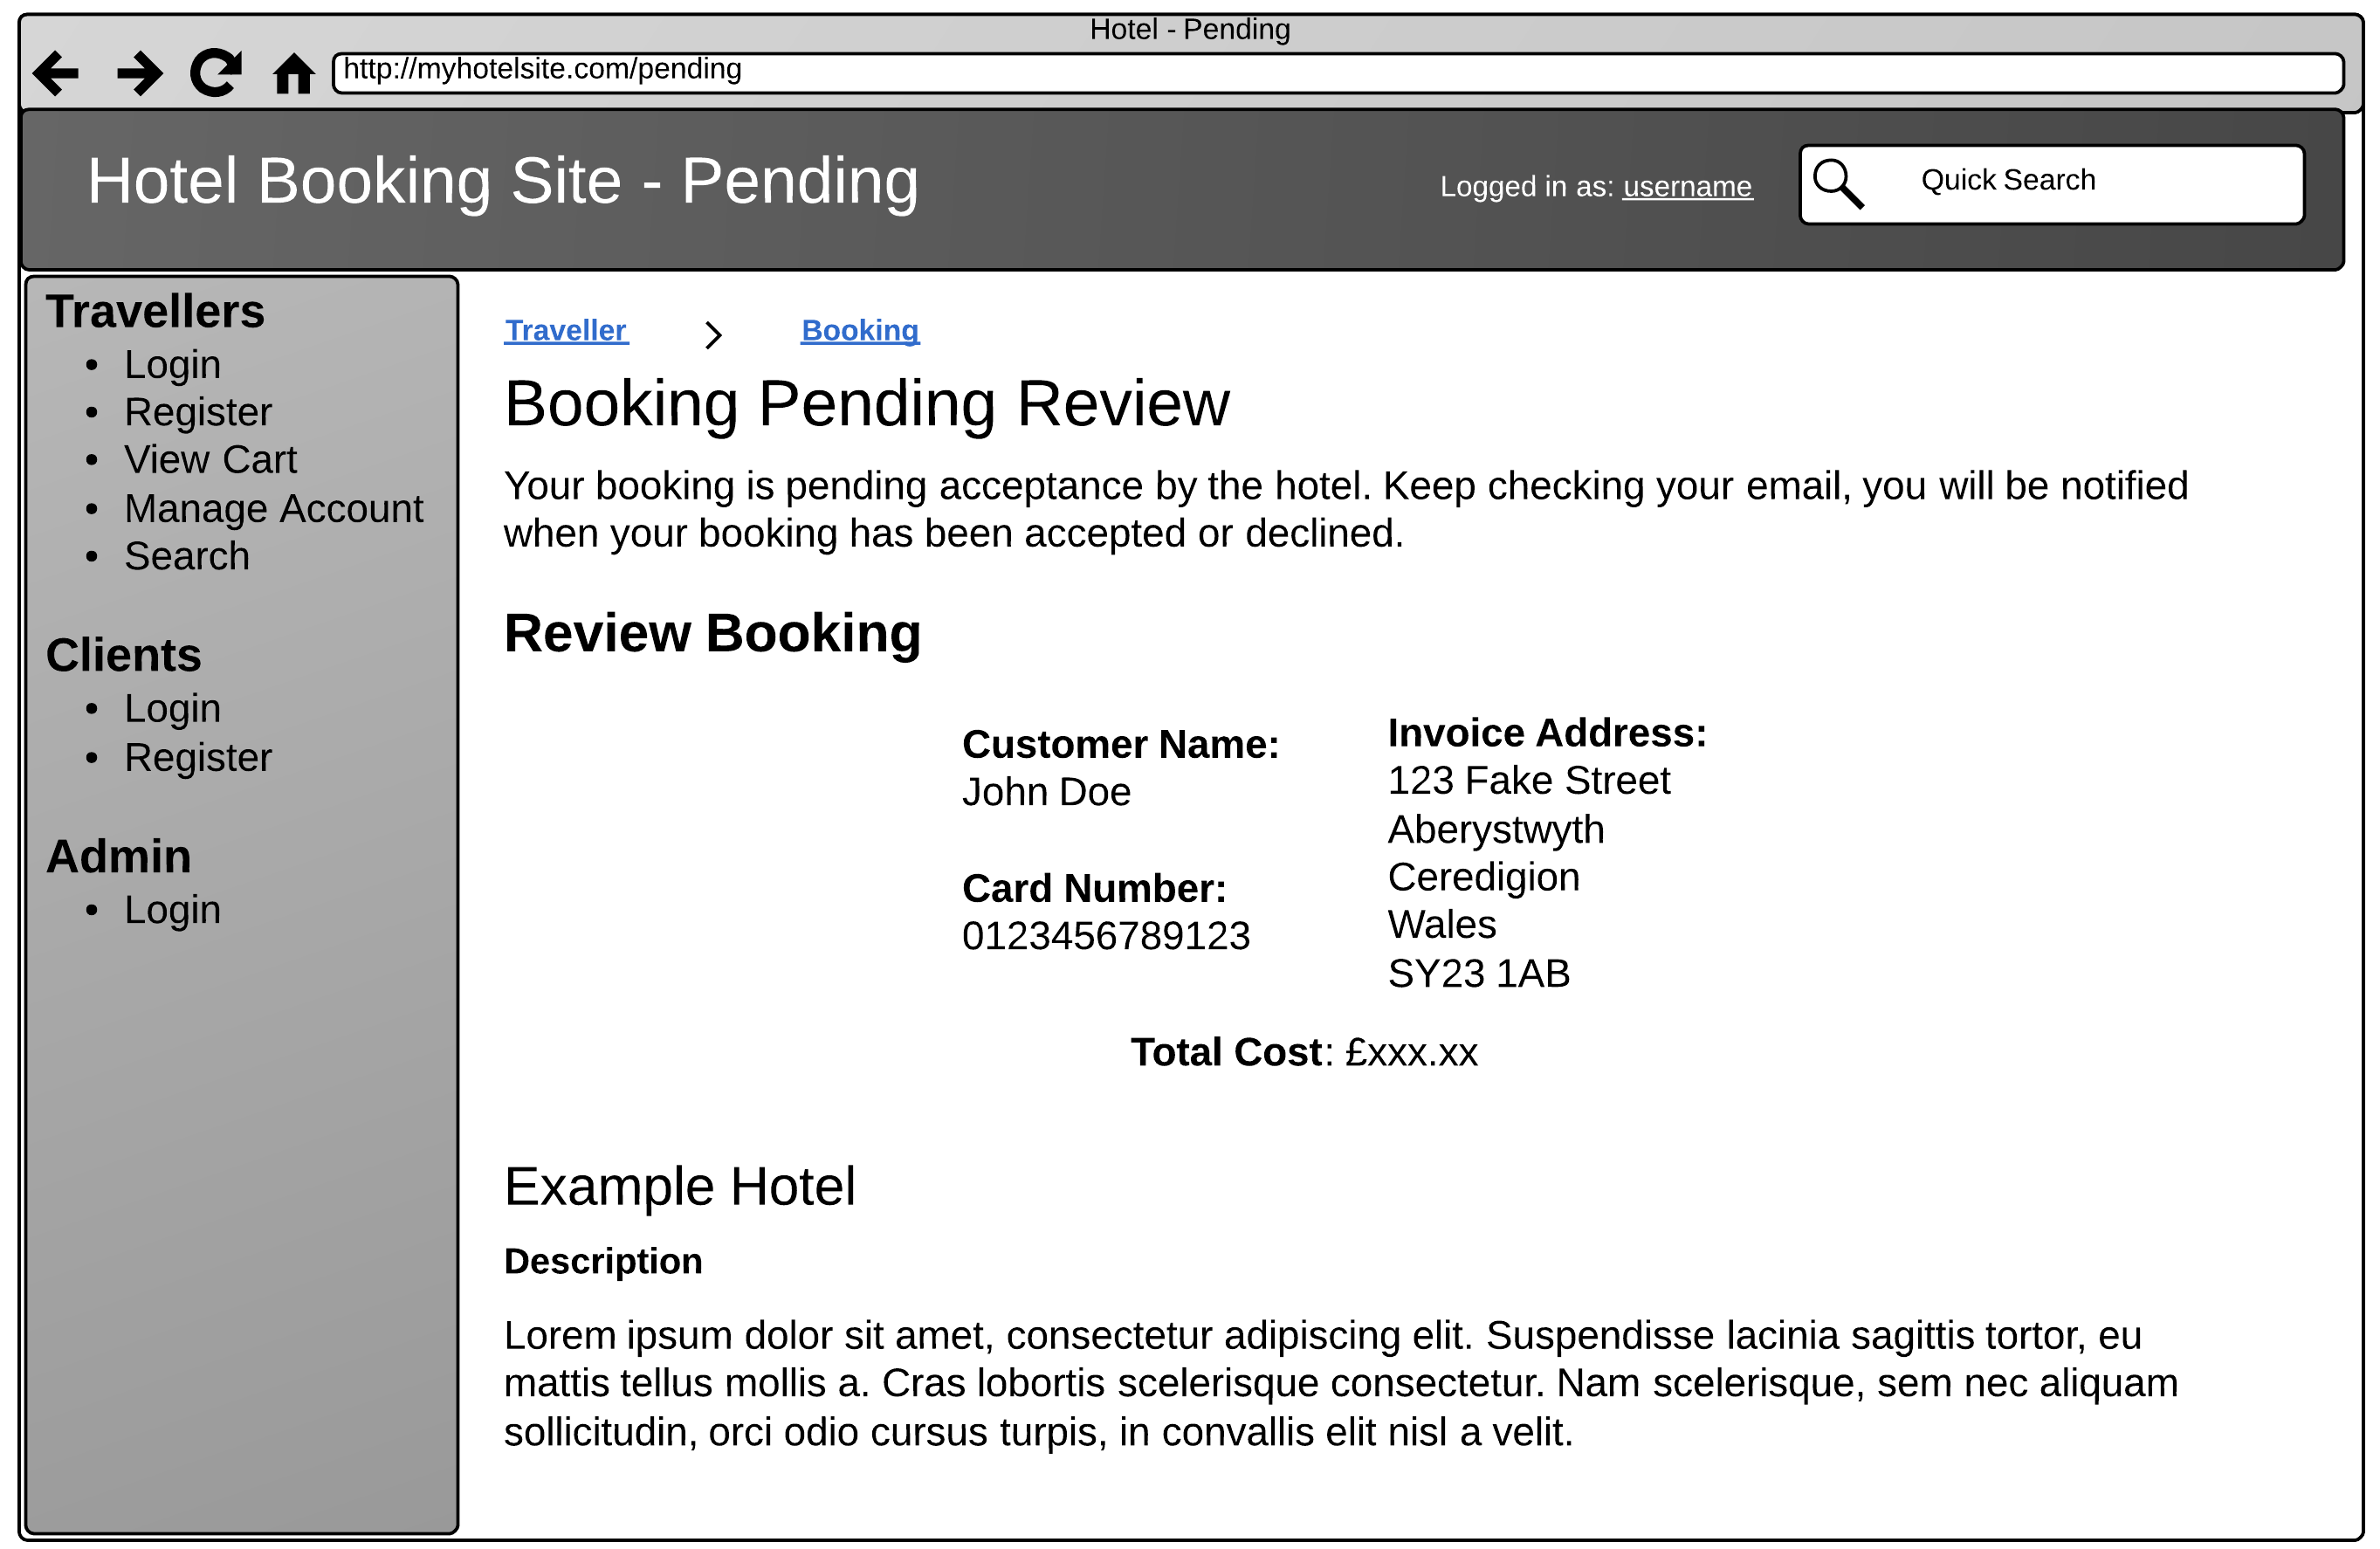
\includegraphics[width=0.7\textwidth]{img/wireframes/Pending.png}
\caption{Wireframe for the page shown on a pending booking.}
\label{fig:wireframe-traveller-pending}
\end{figure}

\section{Prototype}
As mentioned in the first paragraph of this document, a prototype implementation of the site outlined by this task analysis is available at \url{http://users.aber.ac.uk/slj11/cs22310/index.html}. This prototype implements none of the functionality of the proposed site, but does demonstrate the overall structure of the site and the basics of the navigation. 

However, because there is no functionality provided this site does not work the same way as it would if the design were fully realised. For example, the user is not redirected to login/register when they move from the cart to confirm their payment details.

The prototype is also only exactly that, a prototype. If this were a real website, the title of the site would probably be replaced with some custom branding rather than pain text. The company may also require a specific colour scheme rather than the admittedly rather dull grey site. There might also be other requirements such as more detailed search criteria or more customer details required (e.g. telephone number). Finally, the descriptions and textual information available on the site are all either in Lorem Ipsum or are rather short. I have assumed that the content for the site would be provided by site themselves and so for the prototype I have only included place holder text.

\clearpage

\section{Discussion of Accessibility Principles}
In the final section of this document I provide a discussion of how I have given some consideration the to accessibility principles as part of my design for this assignment. While I believe that my design is by no means perfect, I feel that I have managed to demonstrate some simple tips to make it more accessible to a potential diverse audience.

One of the simplest things I have done to make the site more accessible was to ensure that the site validates to according to the W3C XHTML 1.1 specification. While this essentially good web development practice anyway, it also means that specialised tools to aid with accessibility (such as screen readers) will have an easier time parsing the site's underlying HTML. This also means that the site is likely to be parsed correctly on a wider range of devices such mobile phones and tablets that often use custom web browser applications that do not have the advanced mark-up parsing capabilities of fully fledged desktop web browsers.

Leading on from this point I have also validated each page of the site using the online accessibility tool WAVE\footnote{http://wave.webaim.org/} to ensure there a no errors. There were two key points that this tool pointed out I had missed that were not caught by the HTML validator. 

The first was that not all form elements were supplied with an accompanying label tags. While visually it made no sense for some input items to have a label (take a date picker for example), the WAVE pointed out that screen readers would not be able to reader the purpose of the form element to a user. Rather than simply jamming in extra form labels to the design where they were not really needed visually, I created the label tags, but hide them off screen using CSS. This means that the extra text will not be visible to the average user but a screen reader will still read the text as it parses the document. 

The second point highlighted by the WAVE tool was that the pages of the site did not have a content language defined. This meant that any potentially non-English speaking visitors of the site (quite possible with a hotel booking site) who were perhaps using a translation tool on the site (such as google translate) would not be able to auto detect what language the site is in, providing an inconvenience. To solve this I simply added a XHTML document language definition attribute to the html tag.

As a quick side note on international users, this site is has been designed specifically with western users in mind. The reason the navigation menu is on the left hand side is because is the first place a English reader (or any language that reads left to right) will look when exploring a page. It is for this same reasons that during the booking and payment stages the controls to go back a step are positions to the left and the controls to move forward with the transaction are on the right. A person who reads from left to right will see where they have come from and then see where they are going too, hopefully helping the users attention to follow a logical flow rather than jump back and forth across the page.

The site also includes some principles of graceful degradation. This is where newer, more feature rich web browsers get a better user visual experience or enhanced functionality, but older legacy software can still perform all of the tasks on the system. The prototype site for this assignment has two such examples of this. 

Firstly, In order to achieve a page height two column layout (a classic CSS problem) it uses a small piece of JavaScript to expand the columns to the correct height. It also uses it in another part of the site to show a form element based on user input. This could present a problem if the user accessing the site cannot run JavaScript of some reason (such as a mobile device or legacy browser). Secondly in order to give a sense of depth to the design of the pages I have used CSS3 drop shadows to add an extra visual enhancement for the user. CSS3 is not currently a full W3C standard and therefore browsers are not obligated to implement this feature.

However, by utilising the principles of graceful degradation, the site is still fully functional even when JavaScript is turned off. The difference in what the user experiences is that these visual enhancements are simply lost. The navigation and operation in the site is still the same but is not as pleasant as when viewed in browsers that support JavaScript and cutting edge web standards. A good example of the difference can be seen by viewing the site using Microsoft Internet explorer which does not implement CSS3 drop shadow and comparing the difference to how it is displayed in Mozilla Firefox or Google Chrome. 

In further support of legacy machines and as a consideration to mobile devices I have ensured that the content on my site fits into a 800 pixel wide window and that the header and navigation menu is "above the fold" of the site event when scaled down to 600 pixels high. While the only real way to ensure a site displays reasonably on a mobile device is to create a special mobile version, a design that fits into 800x600 pixels should hopefully make it a more comfortable fit, particularly with device such as tablets.

With regards to the general style an design of the site, I feel that it could have been made to be a lot prettier looking that it turned out. However while it is perhaps not the most visually appealing site it does show of some style considerations that incorporate accessibility principles.

Throughout the site I have used only a small collection of colours and in such a way that they highlight specific page elements to the users eye. Take the overall structure of the typical page for example. It is split into three clear sections in the classic header-sidebar-content layout that will be familiar to most web users of almost any experience. These areas are clearly highlighted using three different colour levels and (where CSS3 is available) using a drop shadow to further contrast the dynamic part of the page from the static part.

Any direct input from the user in the system is taken in using forms which I have styled to have a consistent look and feel across the whole site. For example text boxes, drop down menus and date pickers are all the small width and have the same degree of padding across the expanse of the site. I have ensured that most form elements are clearly labelled and of that they are all of a type appropriate to the expected input (e.g. using a drop down for month name instead of getting the user to type it). 

Because form elements have been properly encapsulated in form tags, they user can tab through the fields rather than having to move the mouse to click each field, which is great for competent power users. This has the additional benefit of being easier for disabled users who might find it easier to user a keyboard instead of a mouse.

Additionally, I have also tried to enforce a a couple clear hierarchical organisation through out the site. For example, heading attributes are used through the content of the site, but always starting with a large h1 tag (such as what is used in the header) and getting progressively smaller as the user transcends down the information hierarchy. 

The same is true of the menu. It contains five headings representing the major sections according to the user type which list the major pages the user may want to access within those sections. The idea here was that user would see the large headings and identify with what type of user they are (Traveller, admin etc.). After there attention is drawn, the would then being to scan that area and locate the section they are after.

For consistency, I have also made most of the hyper-links on the site that perform specific tasks (e.g adding an item to the cart) look the same as the submit buttons in forms. This is so a user clearly relates the page elements that are in the format of a button as being something that initiates an action with the site. Where I have not made hyper-links conform to this style I have abided by the web standard of simply displaying them with an underline.

In conclusion, I feel that while the site I have produced for this assignment may not be visually spectacular, underneath the hood there has been quite a lot of thought put into accessibility principles. However, i feel that there could still be many improvements made to this site. 

One idea would be to include some kind of structure that clearly shows a Traveller where they are in the paying and booking process (e.g. Reviewing, Paying, Booking, Confirmed etc.) in a similar way to how large shopping sites like Amazon do. Another improvement that could be made would be to have alternate versions of the site, such as a mobile version, that would give the Hotel Booking site a greater platform thorough which their content could be properly distributed.

\end{document}